% Options for packages loaded elsewhere
\PassOptionsToPackage{unicode}{hyperref}
\PassOptionsToPackage{hyphens}{url}
%
\documentclass[
]{book}
\usepackage{amsmath,amssymb}
\usepackage{iftex}
\ifPDFTeX
  \usepackage[T1]{fontenc}
  \usepackage[utf8]{inputenc}
  \usepackage{textcomp} % provide euro and other symbols
\else % if luatex or xetex
  \usepackage{unicode-math} % this also loads fontspec
  \defaultfontfeatures{Scale=MatchLowercase}
  \defaultfontfeatures[\rmfamily]{Ligatures=TeX,Scale=1}
\fi
\usepackage{lmodern}
\ifPDFTeX\else
  % xetex/luatex font selection
\fi
% Use upquote if available, for straight quotes in verbatim environments
\IfFileExists{upquote.sty}{\usepackage{upquote}}{}
\IfFileExists{microtype.sty}{% use microtype if available
  \usepackage[]{microtype}
  \UseMicrotypeSet[protrusion]{basicmath} % disable protrusion for tt fonts
}{}
\makeatletter
\@ifundefined{KOMAClassName}{% if non-KOMA class
  \IfFileExists{parskip.sty}{%
    \usepackage{parskip}
  }{% else
    \setlength{\parindent}{0pt}
    \setlength{\parskip}{6pt plus 2pt minus 1pt}}
}{% if KOMA class
  \KOMAoptions{parskip=half}}
\makeatother
\usepackage{xcolor}
\usepackage{longtable,booktabs,array}
\usepackage{calc} % for calculating minipage widths
% Correct order of tables after \paragraph or \subparagraph
\usepackage{etoolbox}
\makeatletter
\patchcmd\longtable{\par}{\if@noskipsec\mbox{}\fi\par}{}{}
\makeatother
% Allow footnotes in longtable head/foot
\IfFileExists{footnotehyper.sty}{\usepackage{footnotehyper}}{\usepackage{footnote}}
\makesavenoteenv{longtable}
\usepackage{graphicx}
\makeatletter
\def\maxwidth{\ifdim\Gin@nat@width>\linewidth\linewidth\else\Gin@nat@width\fi}
\def\maxheight{\ifdim\Gin@nat@height>\textheight\textheight\else\Gin@nat@height\fi}
\makeatother
% Scale images if necessary, so that they will not overflow the page
% margins by default, and it is still possible to overwrite the defaults
% using explicit options in \includegraphics[width, height, ...]{}
\setkeys{Gin}{width=\maxwidth,height=\maxheight,keepaspectratio}
% Set default figure placement to htbp
\makeatletter
\def\fps@figure{htbp}
\makeatother
\setlength{\emergencystretch}{3em} % prevent overfull lines
\providecommand{\tightlist}{%
  \setlength{\itemsep}{0pt}\setlength{\parskip}{0pt}}
\setcounter{secnumdepth}{5}
\usepackage{booktabs}
\ifLuaTeX
  \usepackage{selnolig}  % disable illegal ligatures
\fi
\usepackage[]{natbib}
\bibliographystyle{apalike}
\usepackage{bookmark}
\IfFileExists{xurl.sty}{\usepackage{xurl}}{} % add URL line breaks if available
\urlstyle{same}
\hypersetup{
  pdftitle={Carbohydrate metabolism for medical students},
  pdfauthor={Padmanaban, Associate Professor, Biochemistry, CMC, Vellore},
  hidelinks,
  pdfcreator={LaTeX via pandoc}}

\title{Carbohydrate metabolism for medical students}
\author{Padmanaban, Associate Professor, Biochemistry, CMC, Vellore}
\date{2024-12-16}

\begin{document}
\maketitle

{
\setcounter{tocdepth}{1}
\tableofcontents
}
\chapter{Introduction}\label{introduction}

The lectures on carbohydrate metabolism are organized as four sections:

Part 1 -- \hyperref[Digestion]{Digestion, absorption, uptake of glucose into tissues}

Part 2 -- Glucose utilization, energy generation and glucose production, regulation of blood glucose levels

\begin{itemize}
\tightlist
\item
  \hyperref[glycolysis]{Glycolysis}
\item
  \hyperref[tca-cycle]{TCA cycle}
\item
  \hyperref[glycogen-metabolism]{Glycogen metabolism}
\item
  \hyperref[gluconeogenesis]{Gluconeogenesis}
\item
  \hyperref[regulation-of-blood-glucose]{Regulation of blood glucose}
\end{itemize}

Part 3 -- Diabetes mellitus and hypoglycemia

\begin{itemize}
\tightlist
\item
  \hyperref[hypoglycemia]{Hypoglycemia}
\item
  \hyperref[diabetes-mellitus]{Diabetes mellitus}
\end{itemize}

Part 4 -- Other pathways and their importance

\begin{itemize}
\tightlist
\item
  \hyperref[hmp-pathway]{HMP Pathway}
\item
  \hyperref[fructose-metabolism]{Fructose metabolism}
\item
  \hyperref[galactose-metabolism]{Galactose metabolism}
\end{itemize}

\chapter{Digestion, absorption, uptake of glucose into tissues}\label{Digestion}

\section{Carbohydrates in our food}\label{carbohydrates-in-our-food}

The common carbohydrates present in our food are starch, lactose, sucrose, fructose, cellulose and other dietary fibres.

\subsection*{Starch}\label{starch}
\addcontentsline{toc}{subsection}{Starch}

Starch is the most common carbohydrate present in our diet. Starch is abundant in cereals (rice, wheat), tubers (potato) and other vegetables.

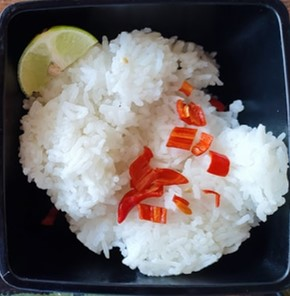
\includegraphics[width=\textwidth,height=2.60417in]{Images/Rice.jpg}

\subsection*{Lactose}\label{lactose}
\addcontentsline{toc}{subsection}{Lactose}

Lactose is present in milk and milk containing products.

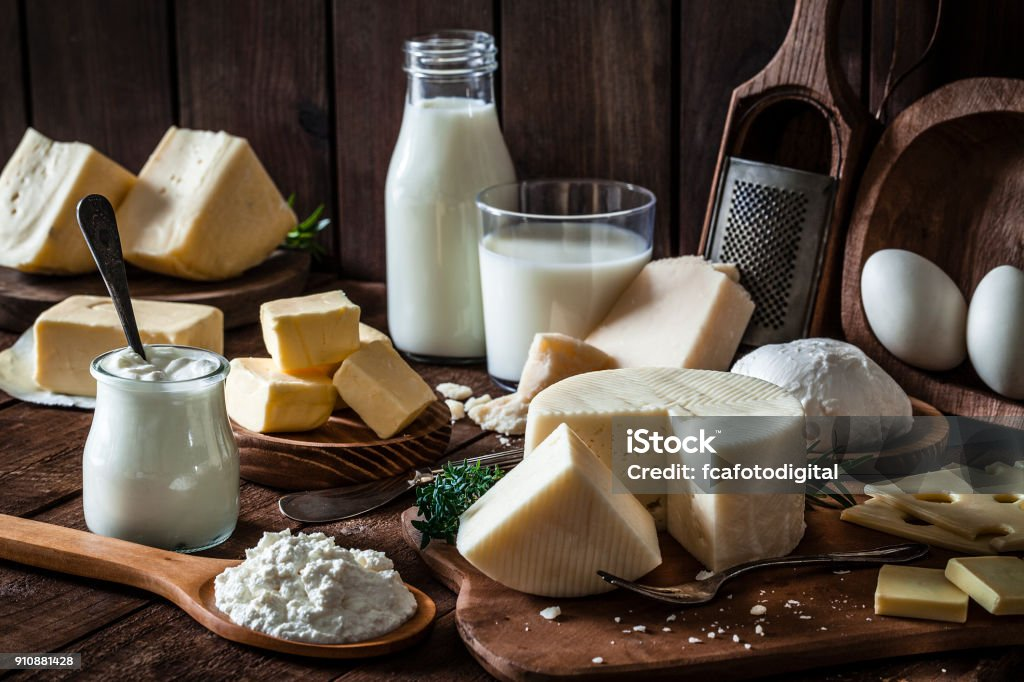
\includegraphics[width=0.5\textwidth,height=\textheight]{Images/Diary.jpg}

\subsection*{Fructose}\label{fructose}
\addcontentsline{toc}{subsection}{Fructose}

Fructose is present in honey and fruits.

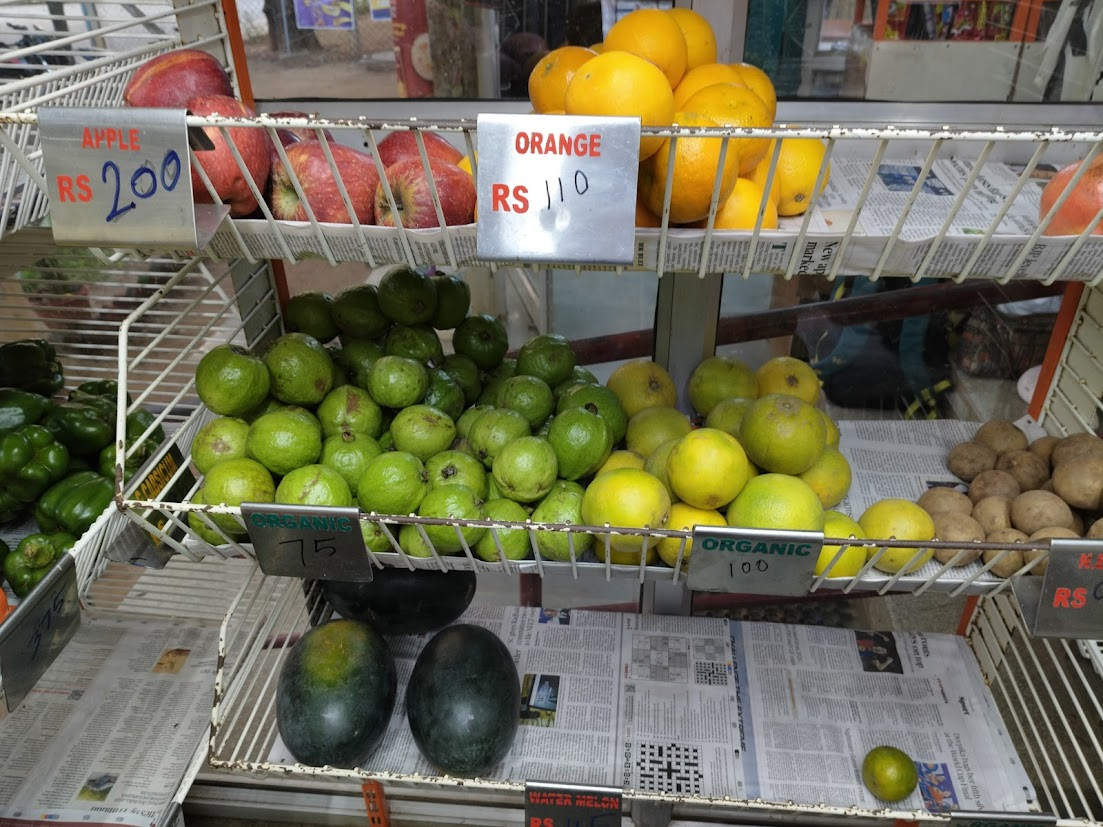
\includegraphics[width=0.5\textwidth,height=\textheight]{Images/Fruit.jpg}

\subsection*{Sucrose}\label{sucrose}
\addcontentsline{toc}{subsection}{Sucrose}

Sucrose is present in sugar and fruits.

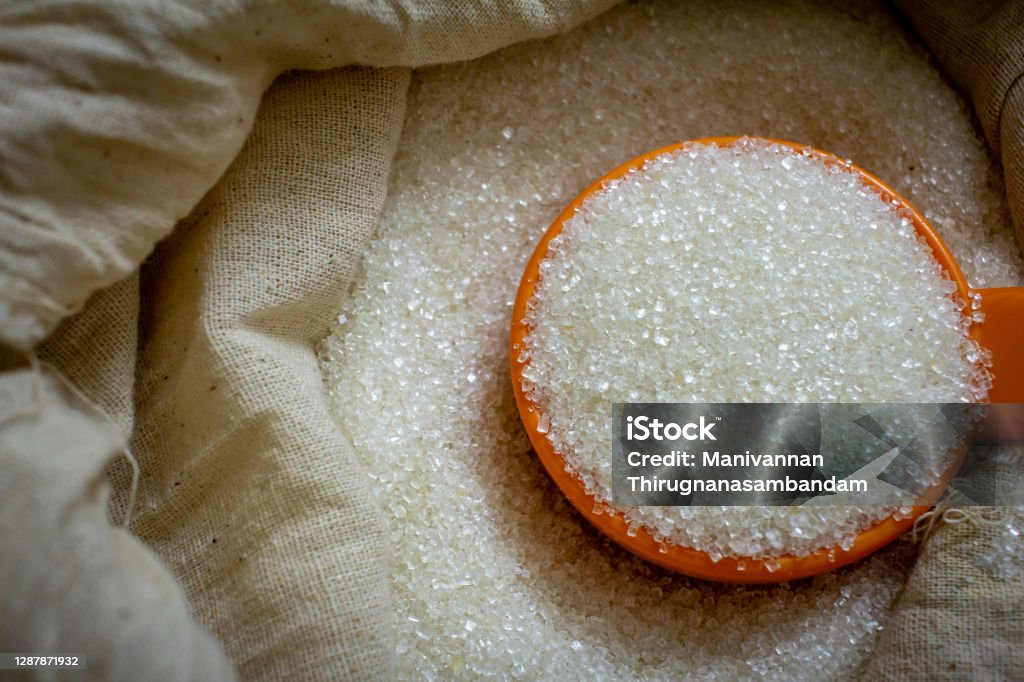
\includegraphics[width=0.5\textwidth,height=\textheight]{Images/Sugar.jpg}

\subsection*{Cellulose}\label{cellulose}
\addcontentsline{toc}{subsection}{Cellulose}

Cellulose and other dietary fibres are present in green leafy vegetables, whole grains, and fruits.

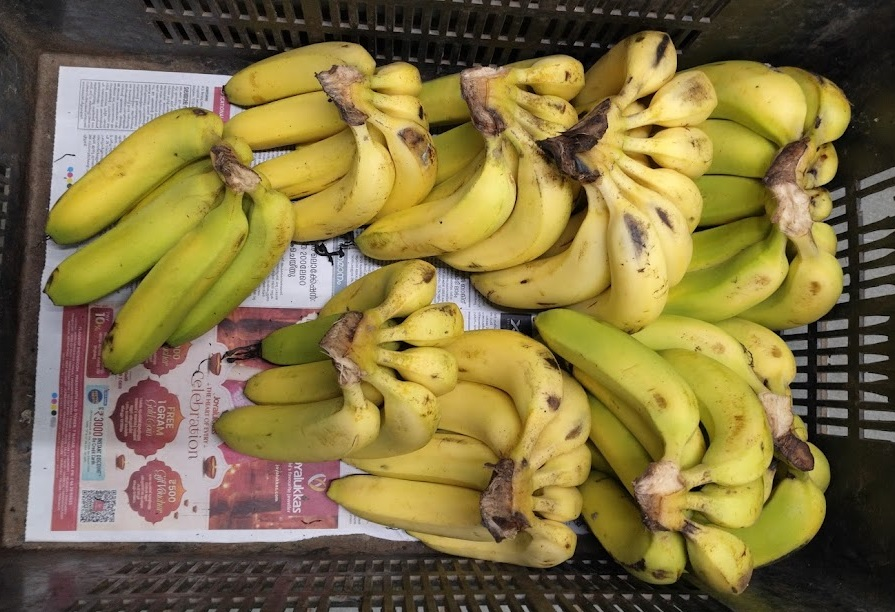
\includegraphics[width=0.5\textwidth,height=\textheight]{Images/Fibre.jpg}

\href{padmanaban55.github.io/CarbohydrateContent}{Explore carbohydrate content in Indian food}

\section{Digestion of carbohydrates}\label{digestion-of-carbohydrates}

The purpose of digestion is to breakdown large polymers into their monomers so that they can transported across the plasma membrane of the intestinal cells into the body. Digestion of carbohydrates converts polysaccharides and disaccharides into \emph{monosaccharides} which can be transported across the intestinal cell (enterocytes). Digestion of carbohydrates is achieved by the enzymes; Salivary and pancreatic amylases, and intestinal disaccharidases.

\subsection{Digestion of starch by amylase}\label{digestion-of-starch-by-amylase}

Digestion of carbohydrates begins in the mouth. Salivary glands secrete the enzyme salivary amylase, and salivary amylase breaks down the polysaccharide starch into smaller pieces. When the food enters the stomach, the acidic pH of the stomach inactivates amylase and so carbohydrate digestion does not happen in stomach. When the food leaves stomach and enters duodenum, it will be acted upon by pancreatic amylase secreted by pancreas.Pancreatic amylase digests the remaining starch (and glycogen) into dextrins, oligosaccharides and disaccharides.

Amylase breaks 1 to 4 glycosidic bonds of the starch at random places resulting in smaller version of amylopectin called dextrin, and release of the disaccharide Maltose, isomaltose, and the trisaccharide maltotriose.

\subsection{Digestion of disaccharides by disaccharidases}\label{digestion-of-disaccharides-by-disaccharidases}

The epithelial cells (enterocytes) of the small intestine produce a group of enzymes called disaccharidases along their brush border.

These disaccharidases are:
+Lactase
+Sucrase
+Iso-maltase
+Maltase
+Trehalase

Maltase digests maltose into two units of glucose. The sucrase-isomaltase enzyme complex digests sucrose and isomaltose into glucose and fructose, and two glucose units respectively. The enzyme lactase digests lactose into glucose and galactose.

\section{Absorption of monosaccharides}\label{absorption-of-monosaccharides}

Glucose and galactose are absorbed by enterocytes at the apical surface through sodium-dependent glucose transporter -1 (SGLT-1) (Secondary active transport).

Sodium potassium ATPase located at the basolateral surface of the eneterocytes create a concentration gradient of sodium across the apical surface by pumping sodium out at the basolateral side. Sodium is transported through SGLT-1 along the concentration gradient (higher concentration of sodium in the lumen of intestine to lower concentration of sodium inside the eneterocytes). However, SGLT-1 couples the transport of sodium with transport of glucose across the apical surface against it's concentration gradient. This process is illustrated below.

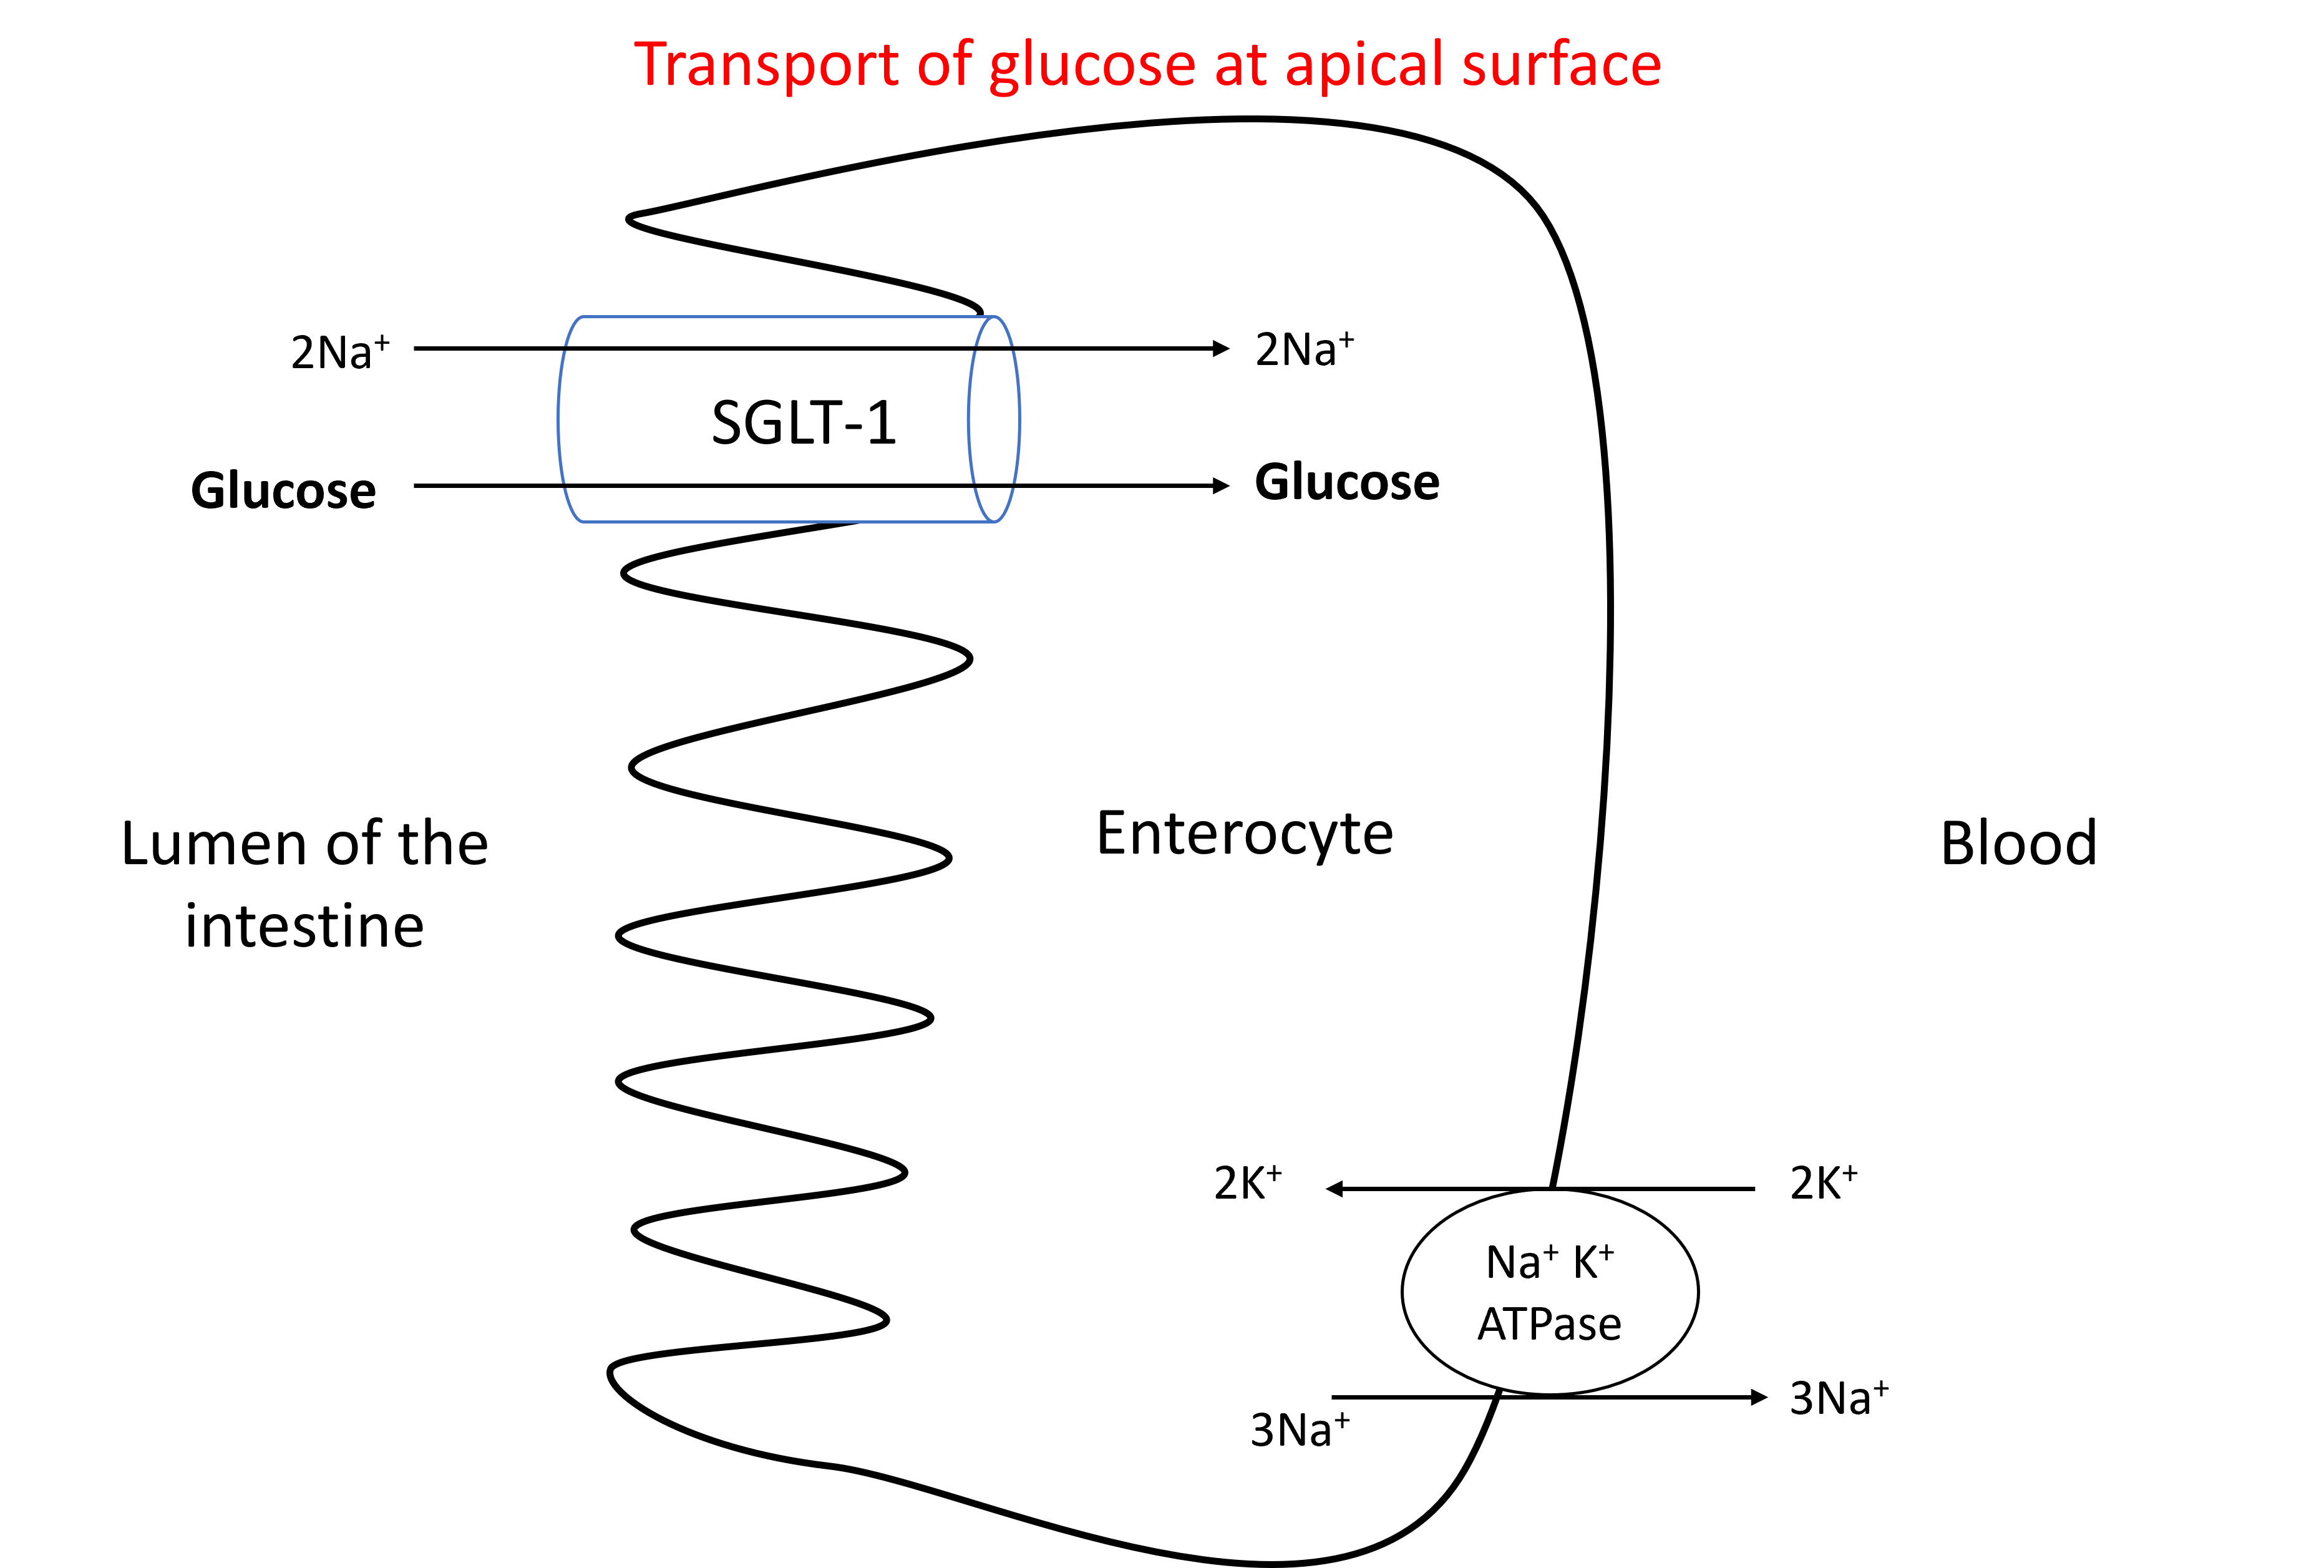
\includegraphics[width=\textwidth,height=4.16667in]{Images/SGLT1.png}

Fructose enters enterocytes through GLUT-5 (Facilitated diffusion) at the apical surface.

Glucose, galactose, and fructose are transported into the blood from enterocytes (basal surface) through GLUT-2 (Facilitated diffusion).

\section{Glucose transporters}\label{glucose-transporters}

Glucose is transported across plasma membrane of cells by transport proteins. Broadly there two families of glucose transporters: Sodium-dependent glucose transporter family (SGLT) and Glucose transporter family (GLUT). SGLT transporters act via secondary active transport and is present in intestine and kidney.

GLUT family of transporters are involved in facilitated diffusion of glucose and other hexoses. There are 14 different types of GLUT proteins. Different types of GLUT are present in different types of tissues which differ in the kinetics of transport and their regulation. These differences reflect the physiological role of the tissues in carbohydrate metabolism. The table below illustrates this concept with important examples.

\begin{longtable}[]{@{}
  >{\raggedright\arraybackslash}p{(\columnwidth - 4\tabcolsep) * \real{0.2258}}
  >{\centering\arraybackslash}p{(\columnwidth - 4\tabcolsep) * \real{0.3871}}
  >{\raggedleft\arraybackslash}p{(\columnwidth - 4\tabcolsep) * \real{0.3871}}@{}}
\toprule\noalign{}
\begin{minipage}[b]{\linewidth}\raggedright
Transporter
\end{minipage} & \begin{minipage}[b]{\linewidth}\centering
Tissue distribution
\end{minipage} & \begin{minipage}[b]{\linewidth}\raggedleft
Function
\end{minipage} \\
\midrule\noalign{}
\endhead
\bottomrule\noalign{}
\endlastfoot
GLUT-1 & RBCs, blood-brain barrier & Glucose uptake at basal conditions \\
GLUT-2 & Small intestine,Pancreatic beta cells,Liver and kidney & Absorption of glucose, Allows free entry of glucose into the beta cells and liver \\
GLUT-3 & Neurons & High-affinity uptake of glucose by brain and nervous tissue even at lower concentrations \\
GLUT-4 & Adipose tissue, skeletal muscle and heart & Insulin stimulated uptake of glucose \\
\end{longtable}

\href{padmanaban55.github.io/GLUT_Transporters/}{Explore the GLUT transporter app}

\section{Clinical applications}\label{clinical-applications}

\subsection{ORS}\label{ors}

Oral rehydration solution is a combination of glucose and sodium used to treat dehydration (loss of water from body). Presence of glucose aids in the absorption of sodium via SGLT-1. Absorption of sodium is accompanied by absorption of water to maintain osmotic equilibrium. This results in more efficient absorption of water.

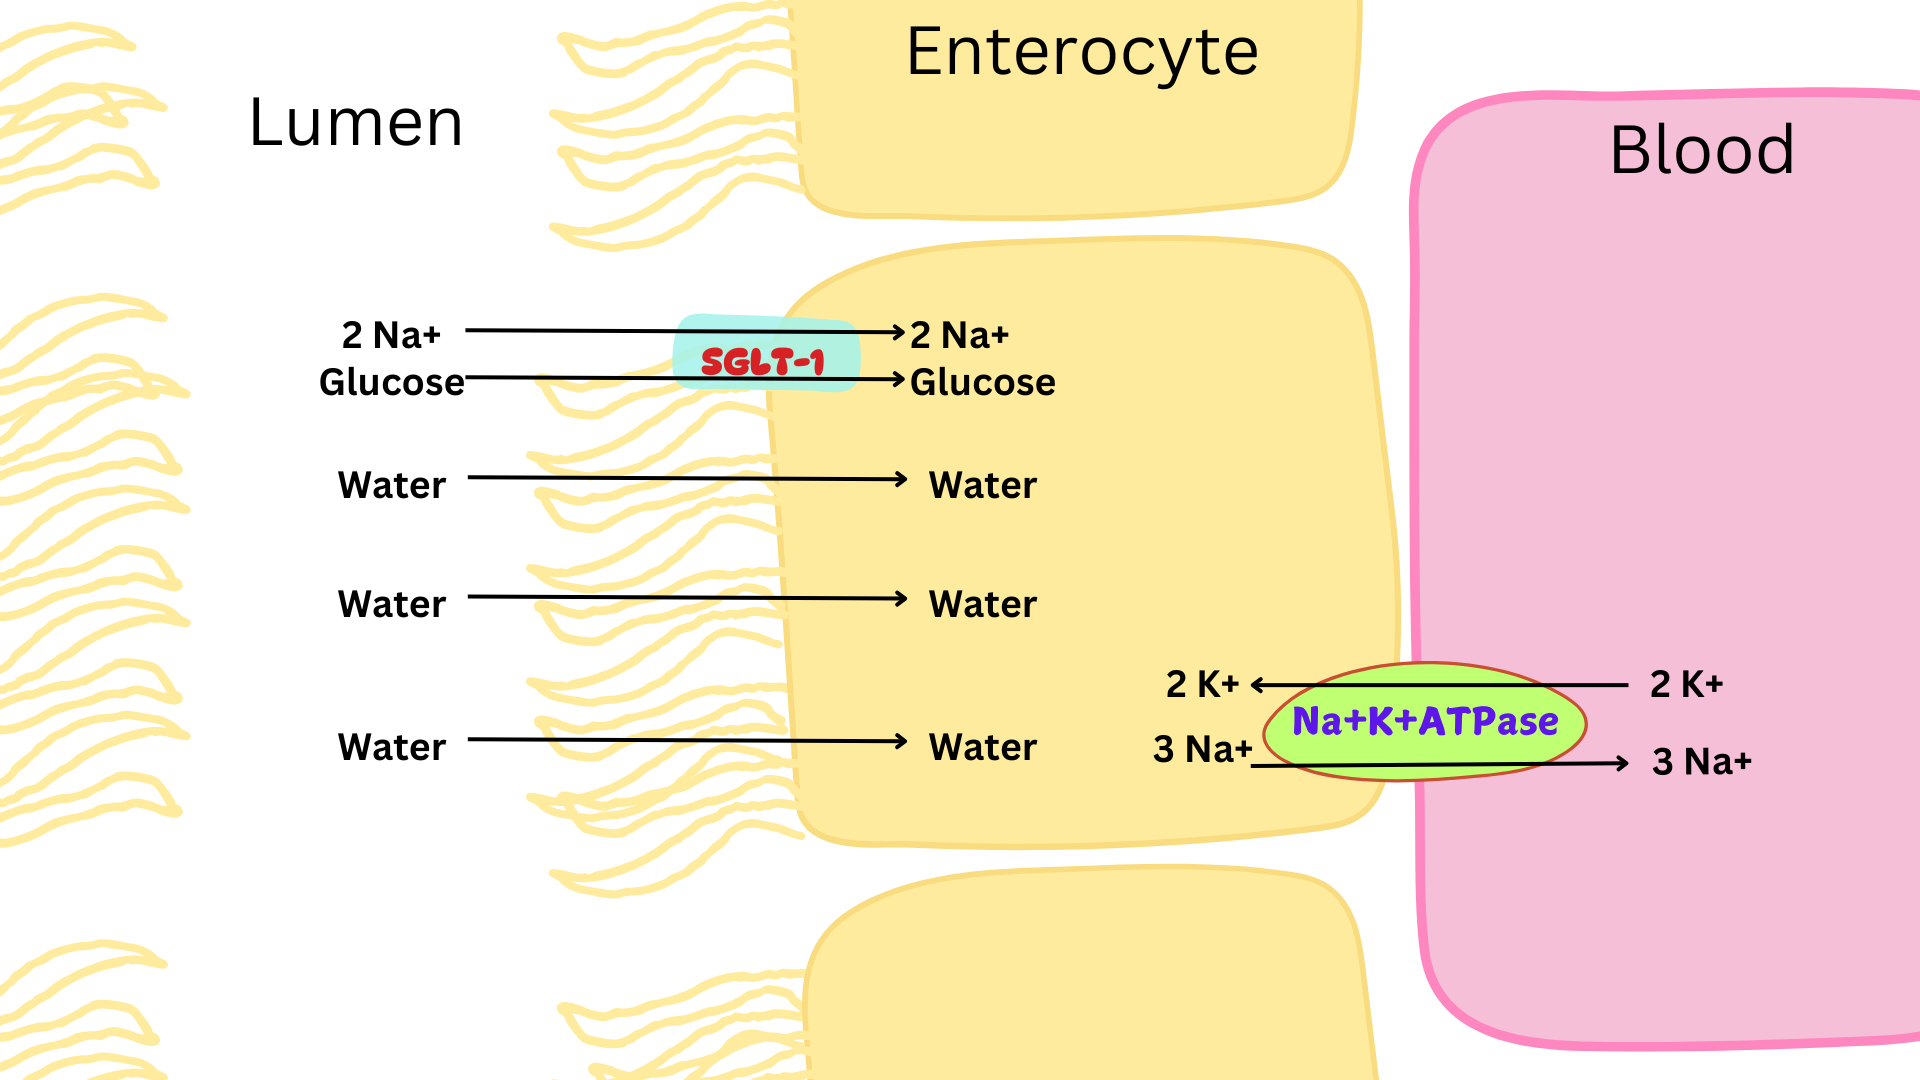
\includegraphics[width=\textwidth,height=4.16667in]{Images/ORS.png}
\footnote{Made by Dr.Monica Peter}

\subsection{Lactose intolerane}\label{lactose-intolerane}

Lactose intolerane occurs due to deficiency of lactase enzyme. The most common reason is lactase non-persistence genotype seen among many populations around the world. The enzyme lactase responsible for digestion of lactose is present during childhood but it's expression declines with age in these populations. Some populations express lactase enzyme well into adulthood due to a genetic mutation and are capable of digesting lactose. Less commonly transient decrease in lactase enzyme due to intestinal diseases can lead to transient lactose intolerance. Rarely, congenital deficiency of lactase enzyme can lead to lactose intolerance in infants.

Clinical features of lactose intolerance includes bloating, abdominal pain, and diarrhea after consuming milk and milk containing products. Undigested lactose is osmotically active which causes increased secretion of water from intestine leading to diarrhea. Undigested lactose is also fermented by the large intestinal bacteria releasing gases in the intestine causing distension and bloating of abdomen. Treatment involves avoiding milk and milk containing food, and if required lactase enzyme supplementation.

\subsection{Dietary fibre}\label{dietary-fibre}

Certain carbohydrate and non-carbohydrates present in plant food that are indigestible are called dietar fibres. Examples: Cellulose, hemicellulose, pectin and lignin. Dietary sources include cereals, whole grains, vegetables, fruits, legumes, bran, and nuts. Some fibres delay gastric emptying and causes increased satiety thus reducing the amount of food intake. Other fibres absorb water and increase the bulk of stool and eases defecation thus preventing constipation. Increased satiety helps in weight reduction. Reduced rate of absorption of glucose due to fibres is beneficial for people with diabetes mellitus.Other benefits include reduction in cholesterol level and reduced risk of colon cancer.

\section{Practice exercises}\label{practice-exercises}

\begin{enumerate}
\def\labelenumi{\arabic{enumi}.}
\tightlist
\item
  Match the carbohydrates with their corresponding digestive enzyme
\end{enumerate}

\begin{itemize}
\item
  ``Sucrose:
\item
  \begin{enumerate}
  \def\labelenumi{(\Alph{enumi})}
  \tightlist
  \item
    Maltase\\
  \end{enumerate}
\item
  \begin{enumerate}
  \def\labelenumi{(\Alph{enumi})}
  \setcounter{enumi}{1}
  \tightlist
  \item
    Amylase\\
  \end{enumerate}
\item
  \begin{enumerate}
  \def\labelenumi{(\Alph{enumi})}
  \setcounter{enumi}{2}
  \tightlist
  \item
    Lactase\\
  \end{enumerate}
\item
  \begin{enumerate}
  \def\labelenumi{(\Alph{enumi})}
  \setcounter{enumi}{3}
  \tightlist
  \item
    Sucrase
  \end{enumerate}
\end{itemize}

''

\begin{itemize}
\item
  ``Starch:
\item
  \begin{enumerate}
  \def\labelenumi{(\Alph{enumi})}
  \tightlist
  \item
    Maltase\\
  \end{enumerate}
\item
  \begin{enumerate}
  \def\labelenumi{(\Alph{enumi})}
  \setcounter{enumi}{1}
  \tightlist
  \item
    Amylase\\
  \end{enumerate}
\item
  \begin{enumerate}
  \def\labelenumi{(\Alph{enumi})}
  \setcounter{enumi}{2}
  \tightlist
  \item
    Lactase\\
  \end{enumerate}
\item
  \begin{enumerate}
  \def\labelenumi{(\Alph{enumi})}
  \setcounter{enumi}{3}
  \tightlist
  \item
    Sucrase
  \end{enumerate}
\end{itemize}

''

\begin{itemize}
\item
  ``Maltose:
\item
  \begin{enumerate}
  \def\labelenumi{(\Alph{enumi})}
  \tightlist
  \item
    Maltase\\
  \end{enumerate}
\item
  \begin{enumerate}
  \def\labelenumi{(\Alph{enumi})}
  \setcounter{enumi}{1}
  \tightlist
  \item
    Amylase\\
  \end{enumerate}
\item
  \begin{enumerate}
  \def\labelenumi{(\Alph{enumi})}
  \setcounter{enumi}{2}
  \tightlist
  \item
    Lactase\\
  \end{enumerate}
\item
  \begin{enumerate}
  \def\labelenumi{(\Alph{enumi})}
  \setcounter{enumi}{3}
  \tightlist
  \item
    Sucrase
  \end{enumerate}
\end{itemize}

''

\begin{itemize}
\item
  ``Lactose:
\item
  \begin{enumerate}
  \def\labelenumi{(\Alph{enumi})}
  \tightlist
  \item
    Maltase\\
  \end{enumerate}
\item
  \begin{enumerate}
  \def\labelenumi{(\Alph{enumi})}
  \setcounter{enumi}{1}
  \tightlist
  \item
    Amylase\\
  \end{enumerate}
\item
  \begin{enumerate}
  \def\labelenumi{(\Alph{enumi})}
  \setcounter{enumi}{2}
  \tightlist
  \item
    Lactase\\
  \end{enumerate}
\item
  \begin{enumerate}
  \def\labelenumi{(\Alph{enumi})}
  \setcounter{enumi}{3}
  \tightlist
  \item
    Sucrase
  \end{enumerate}
\end{itemize}

''

\begin{enumerate}
\def\labelenumi{\arabic{enumi}.}
\setcounter{enumi}{1}
\item
  Green leafy vegetables are a good source of dietary fibres: TRUE / FALSE
\item
  Consumption of which of the following carbohydrate helps in preventing constipation??
\end{enumerate}

\begin{itemize}
\tightlist
\item
  \begin{enumerate}
  \def\labelenumi{(\Alph{enumi})}
  \tightlist
  \item
    Starch\\
  \end{enumerate}
\item
  \begin{enumerate}
  \def\labelenumi{(\Alph{enumi})}
  \setcounter{enumi}{1}
  \tightlist
  \item
    Cellulose\\
  \end{enumerate}
\item
  \begin{enumerate}
  \def\labelenumi{(\Alph{enumi})}
  \setcounter{enumi}{2}
  \tightlist
  \item
    Heparin\\
  \end{enumerate}
\item
  \begin{enumerate}
  \def\labelenumi{(\Alph{enumi})}
  \setcounter{enumi}{3}
  \tightlist
  \item
    Glycogen
  \end{enumerate}
\end{itemize}

\begin{enumerate}
\def\labelenumi{\arabic{enumi}.}
\setcounter{enumi}{3}
\tightlist
\item
  Absorption of glucose at the apical (luminal) side of the enterocyte is through
\end{enumerate}

\begin{itemize}
\tightlist
\item
  \begin{enumerate}
  \def\labelenumi{(\Alph{enumi})}
  \tightlist
  \item
    Primary active transport\\
  \end{enumerate}
\item
  \begin{enumerate}
  \def\labelenumi{(\Alph{enumi})}
  \setcounter{enumi}{1}
  \tightlist
  \item
    Passive diffusion\\
  \end{enumerate}
\item
  \begin{enumerate}
  \def\labelenumi{(\Alph{enumi})}
  \setcounter{enumi}{2}
  \tightlist
  \item
    Secondary active transport\\
  \end{enumerate}
\item
  \begin{enumerate}
  \def\labelenumi{(\Alph{enumi})}
  \setcounter{enumi}{3}
  \tightlist
  \item
    Faciliated diffusion
  \end{enumerate}
\end{itemize}

\chapter{Glycolysis}\label{glycolysis}

\section{Metabolism}\label{metabolism}

Metabolism is defined as the set of all biochemical reactions that sustains life. Metabolic reactions can be classified as catabolism or anabolism. Catabolism is defined as set of reactions that are involved in utilizing chemical energy of nutrients to produce ATP. Anabolism involves reactions that are involved in synthesis of new biomolecules from precursors.

Catabolism involves breakdown of complex molecules into its component building blocks, conversion of building blocks into acetyl CoA and oxidation of acetyl CoA to produce ATP.

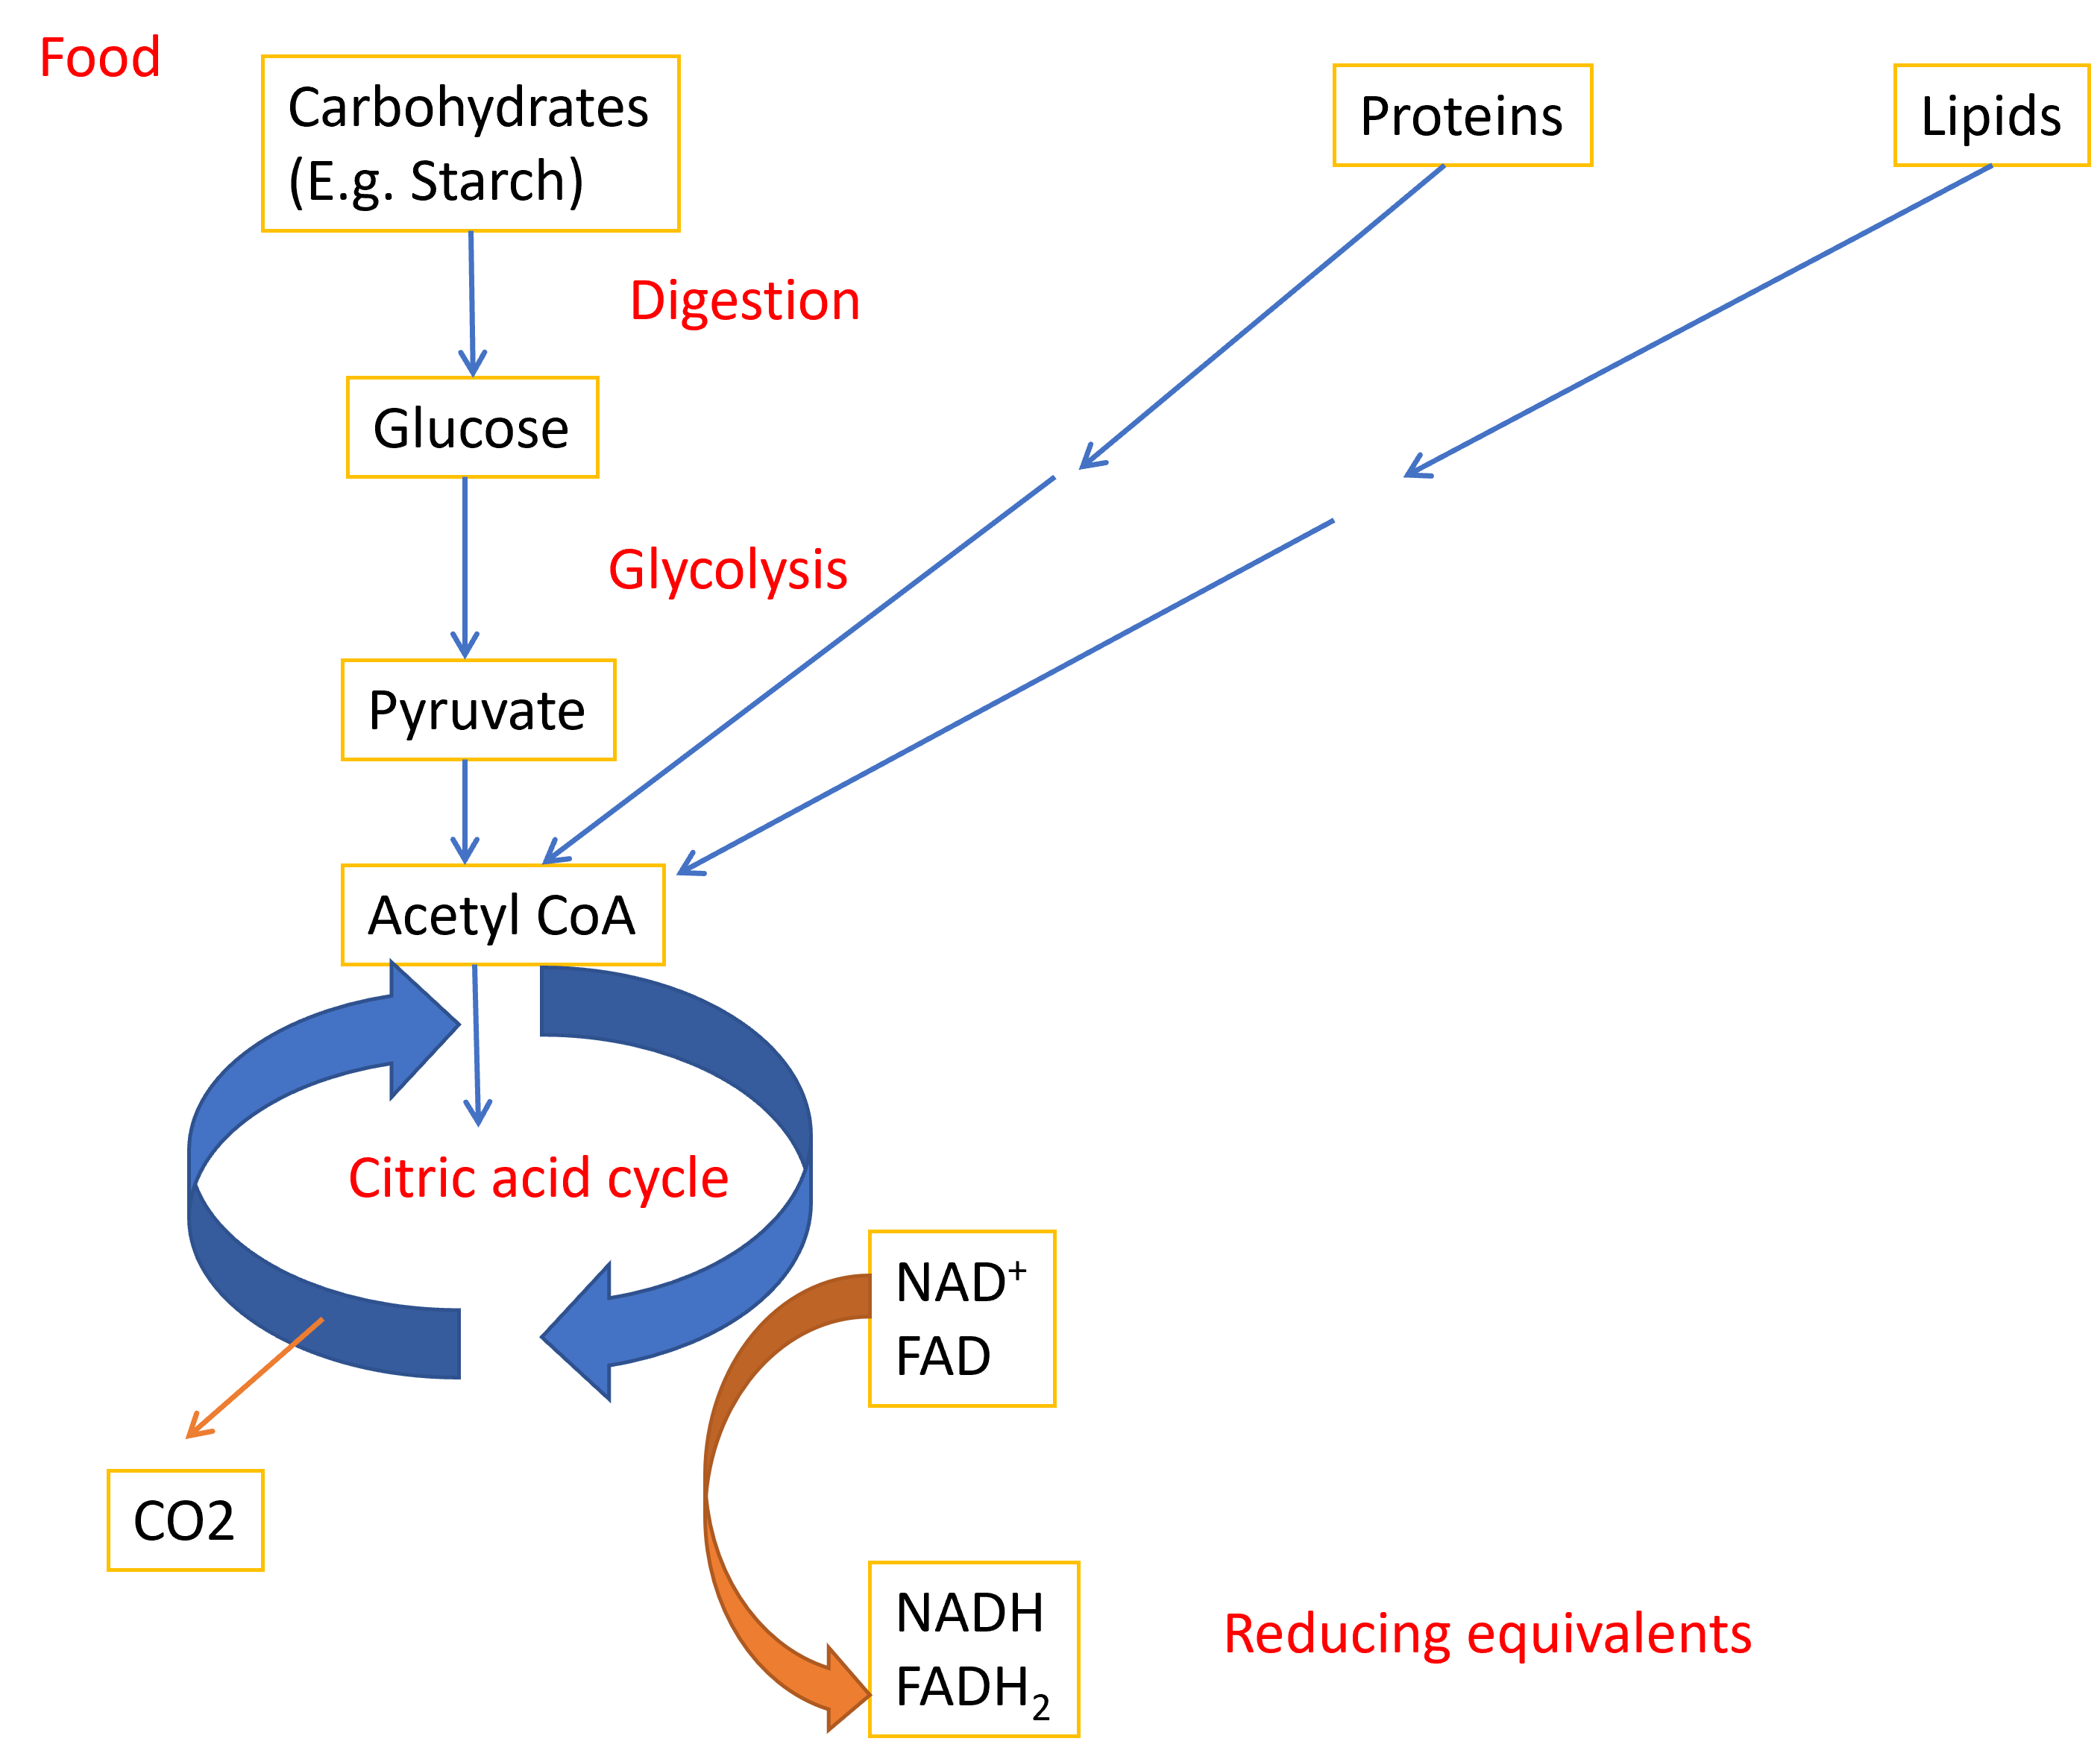
\includegraphics[width=\textwidth,height=4.16667in]{Images/NADH.png}

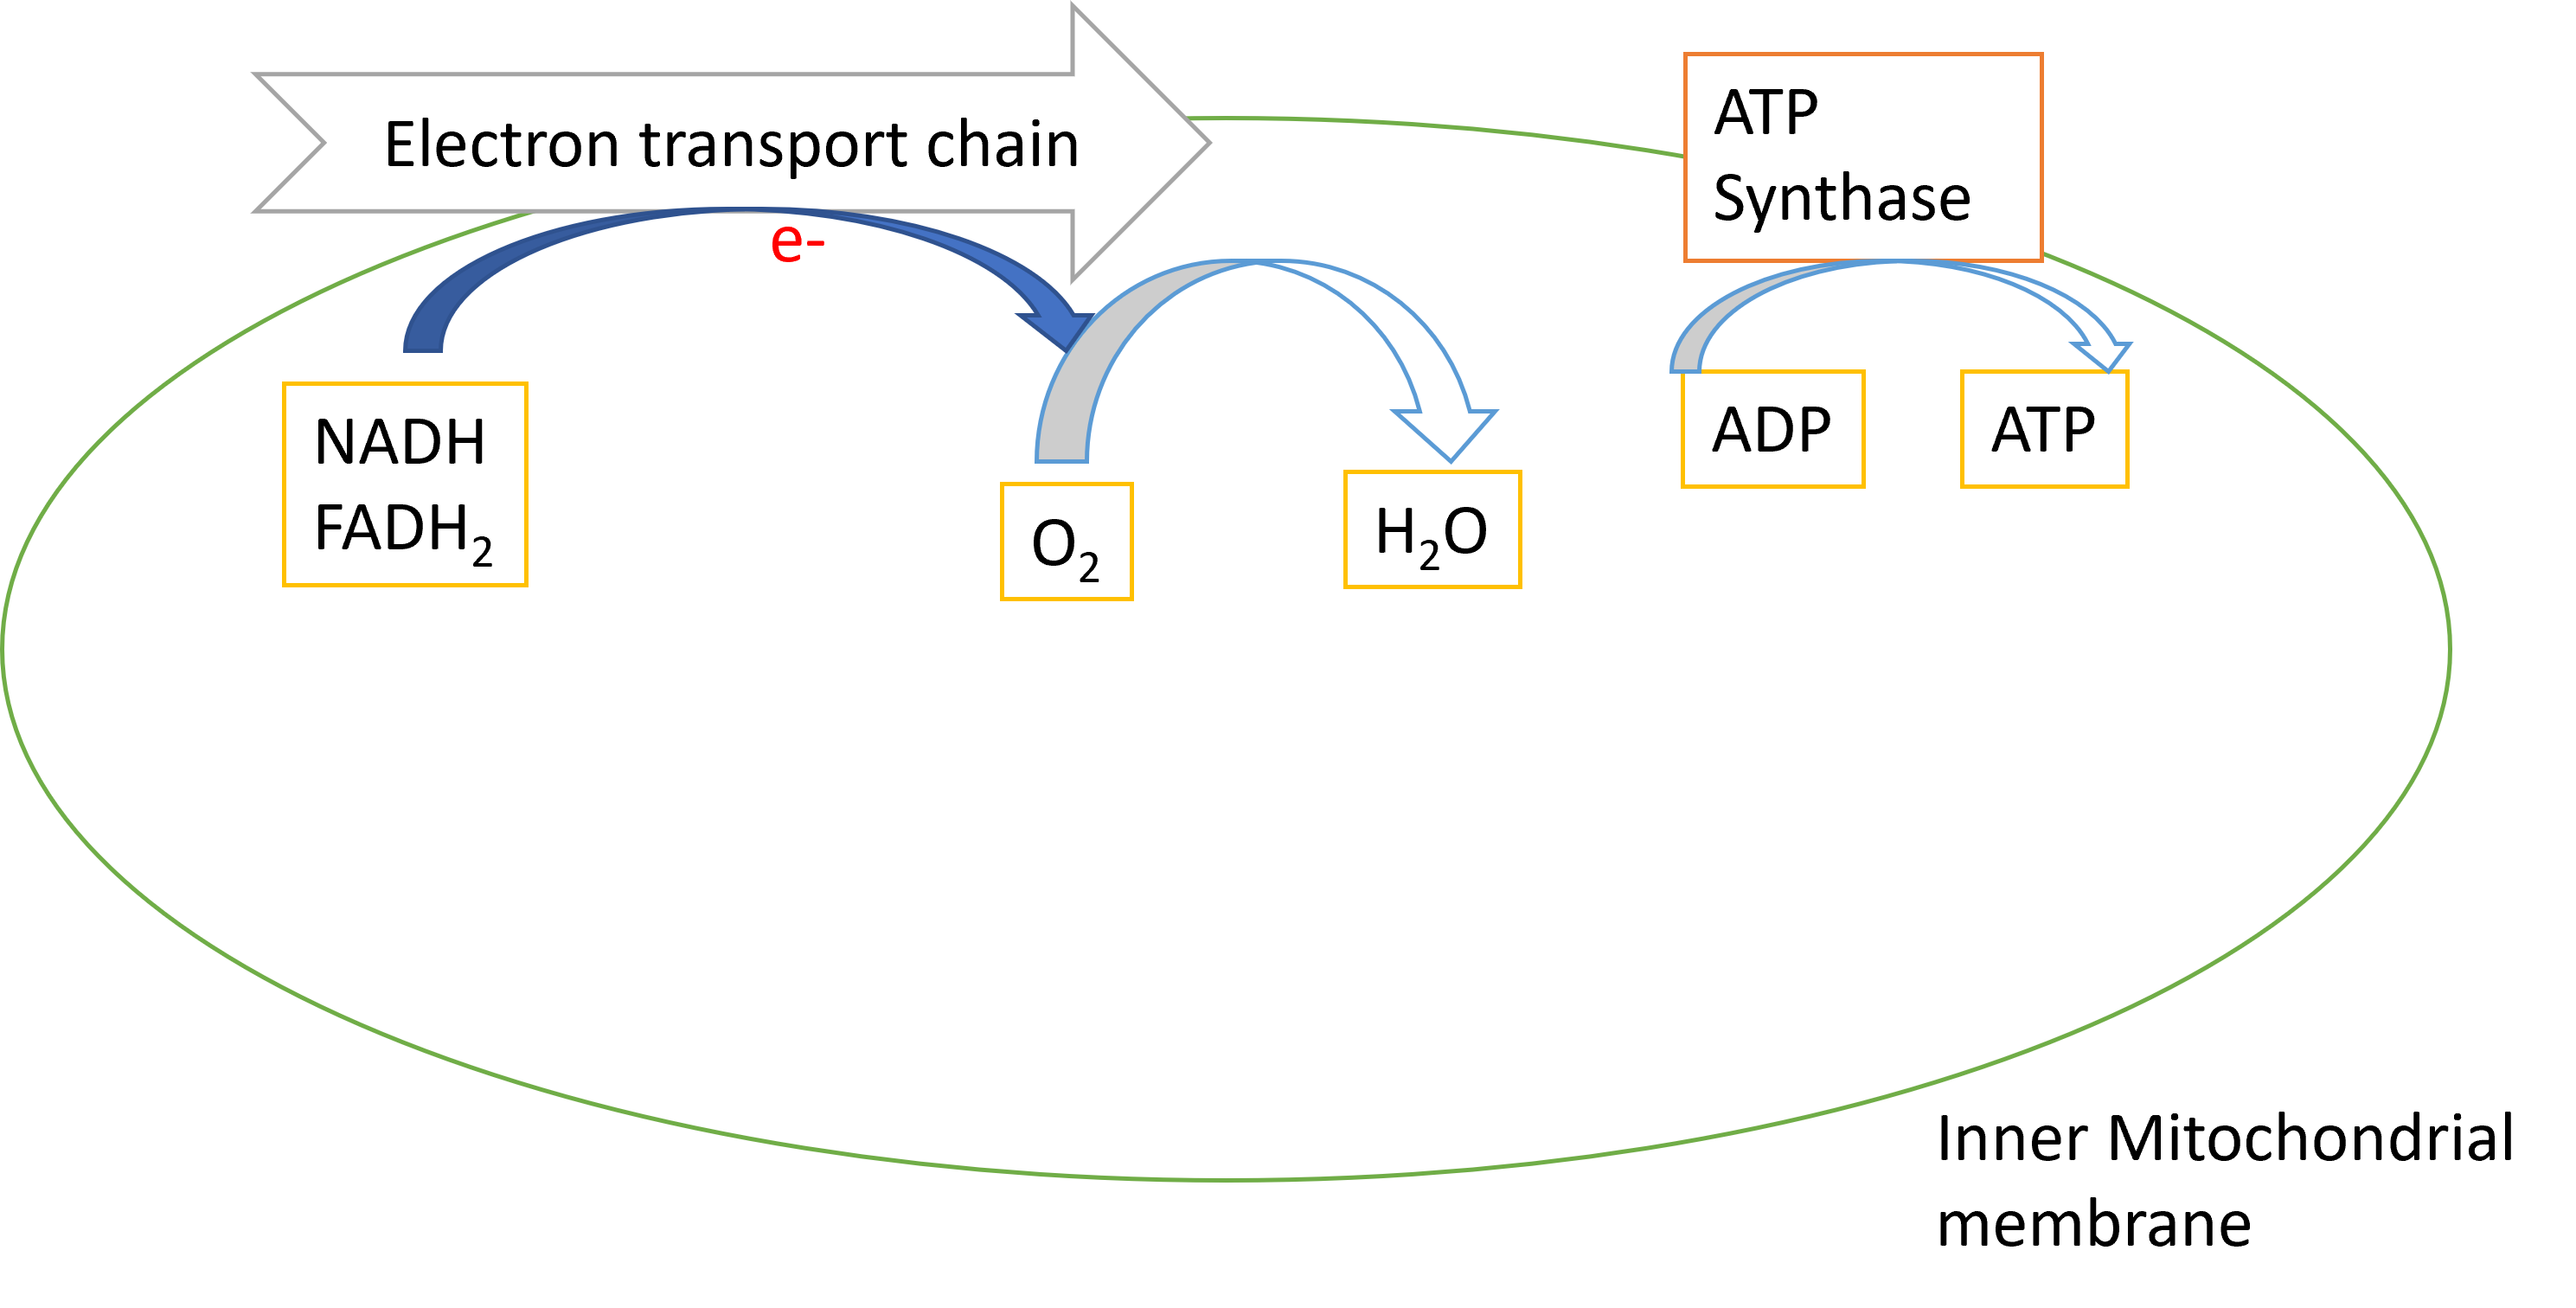
\includegraphics[width=\textwidth,height=2.08333in]{Images/ETC.png}

\section{Overview of carbohydrate metabolism}\label{overview-of-carbohydrate-metabolism}

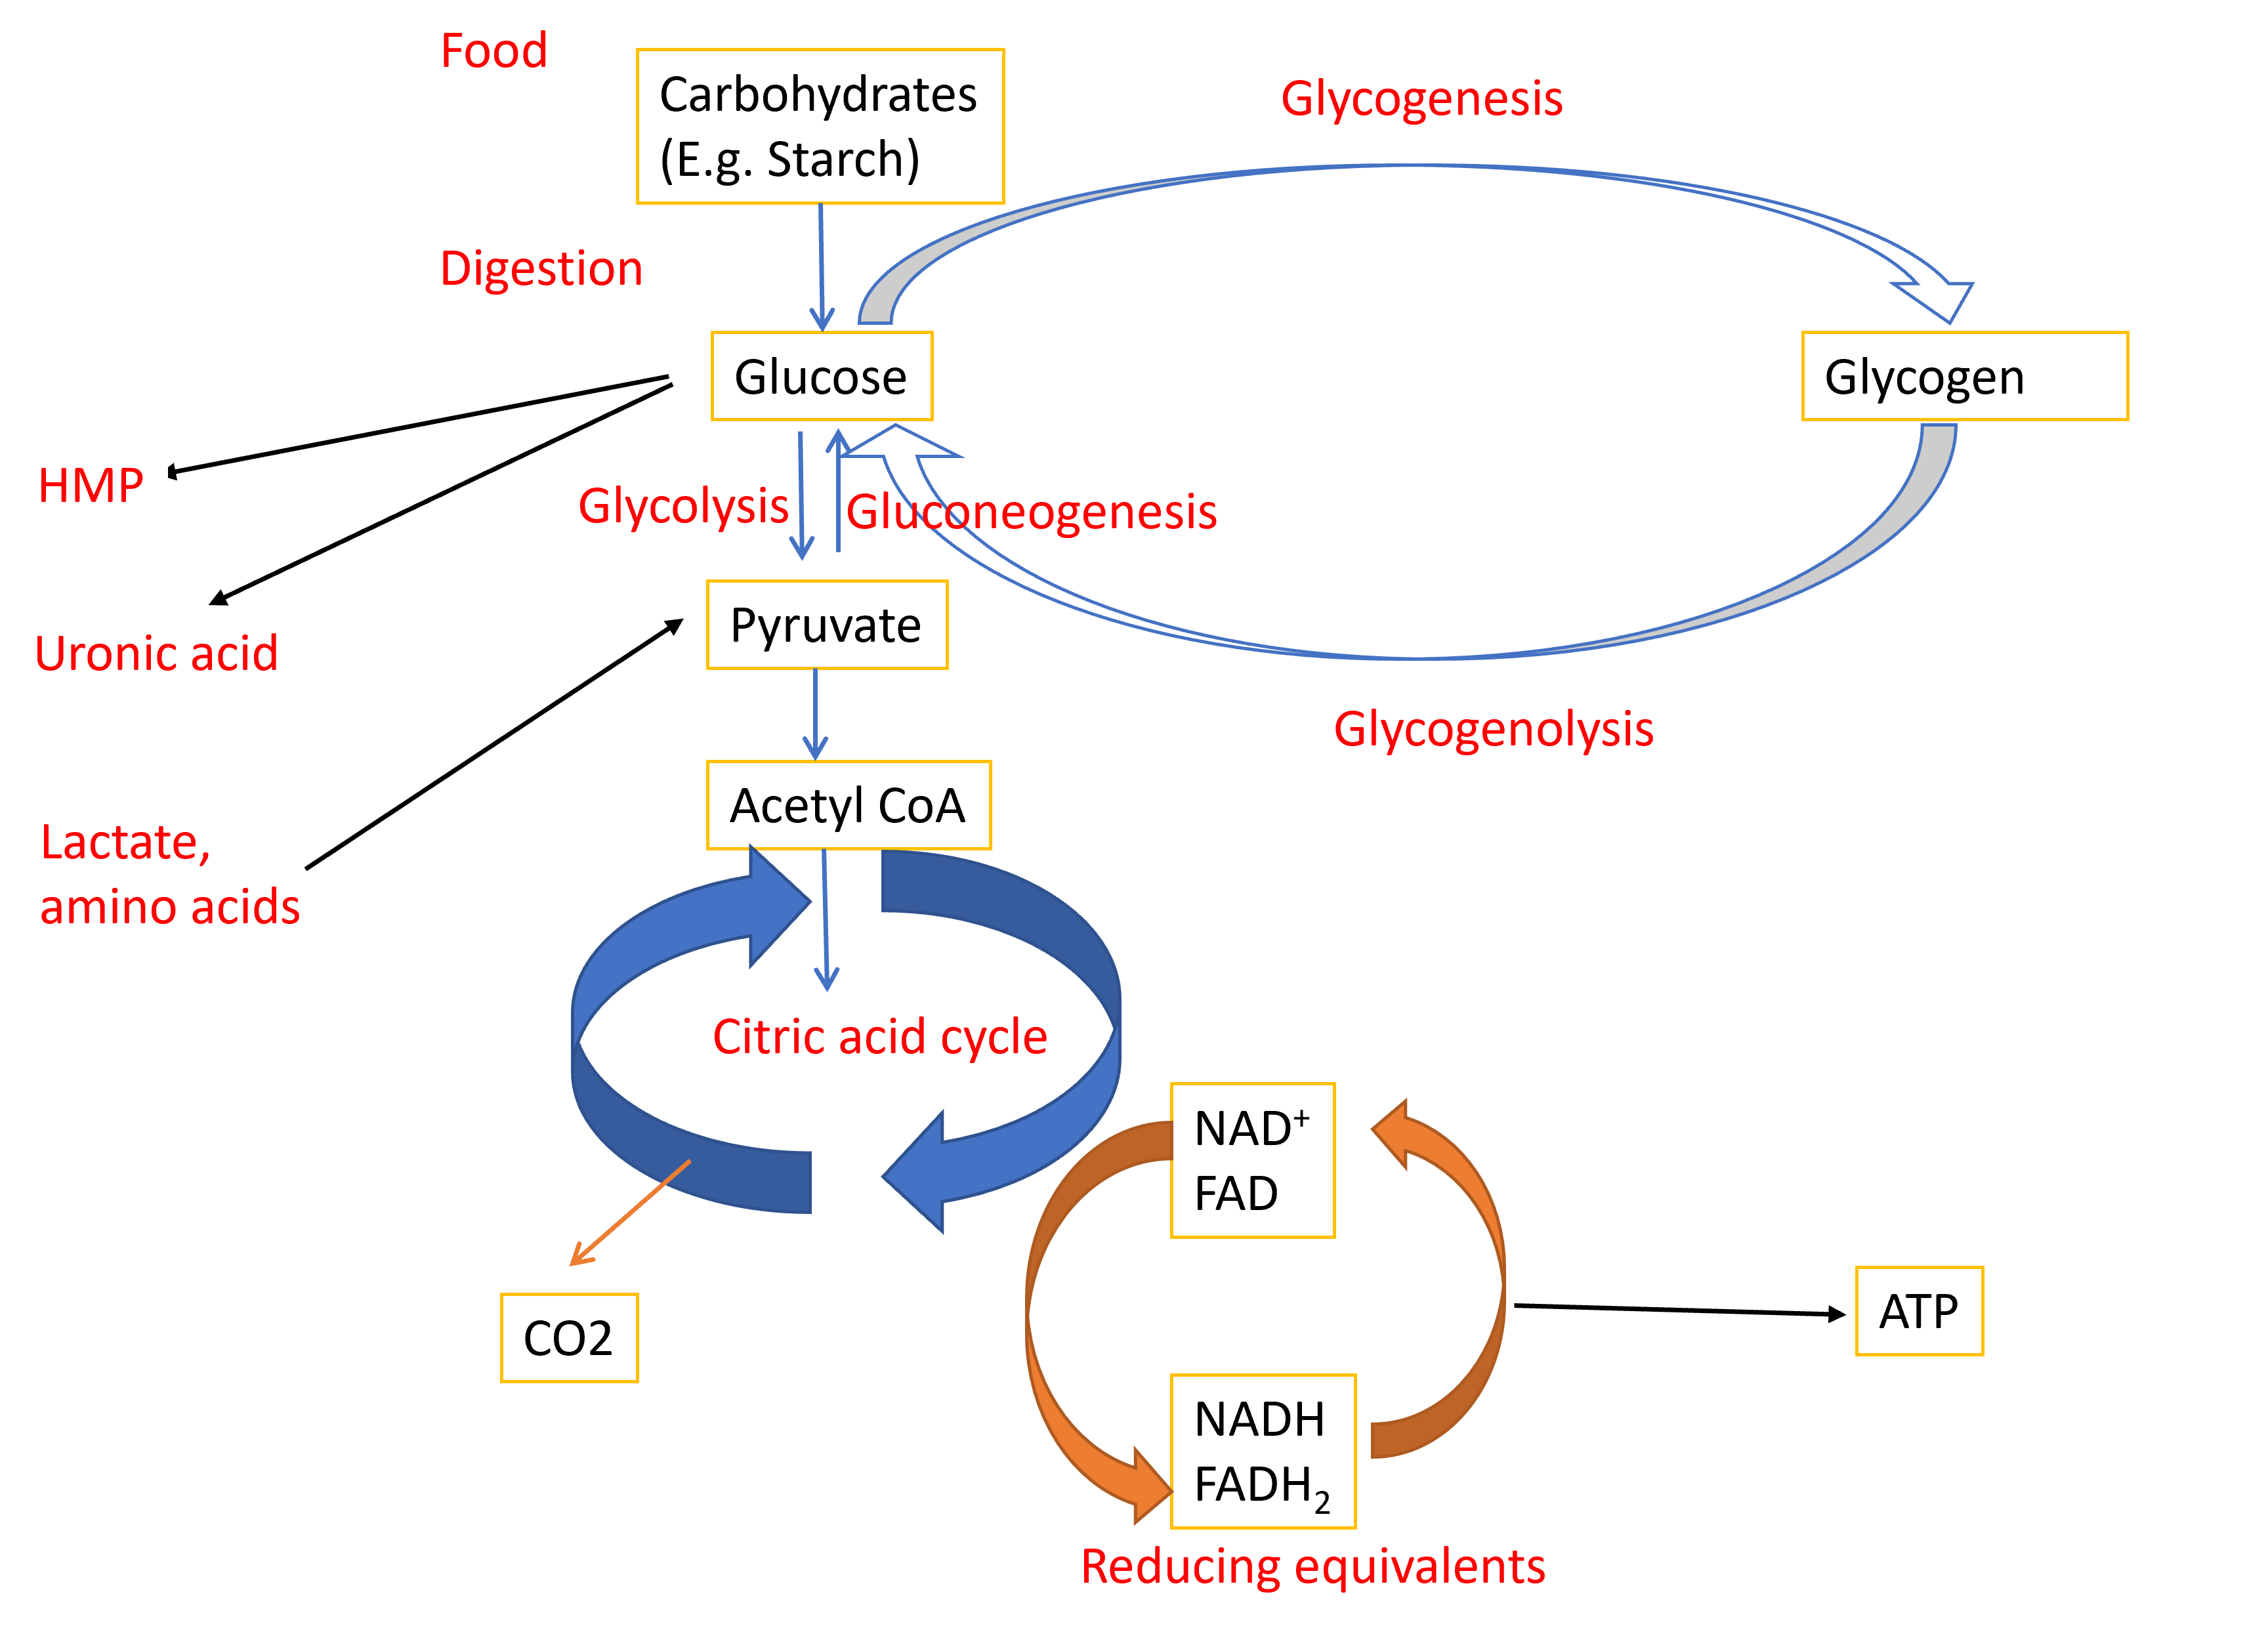
\includegraphics[width=\textwidth,height=4.16667in]{Images/CarbMet.png}

\subsection{Glycolysis}\label{glycolysis-1}

Glycolysis is the major pathway for oxidation of glucose.Glycolysis is the pathway in which glucose is broken down to pyruvate to produce ATP in all tissues.In the presence of oxygen, pyruvate is converted to acetyl-CoA which is further oxidized in citric acid cycle to produce ATP In the absence of oxygen, pyruvate is converted to lactate

\subsection{Reactions of glycolysis}\label{reactions-of-glycolysis}

First 5 steps of glycolysis involves activation of glucose by phosphorylation in two steps and lysis to release two molecules of Glyceraldehyde-3-phosphate which is a 3 carbon molecule. This phase requires investment of 2 ATPs.

\begin{figure}
\centering
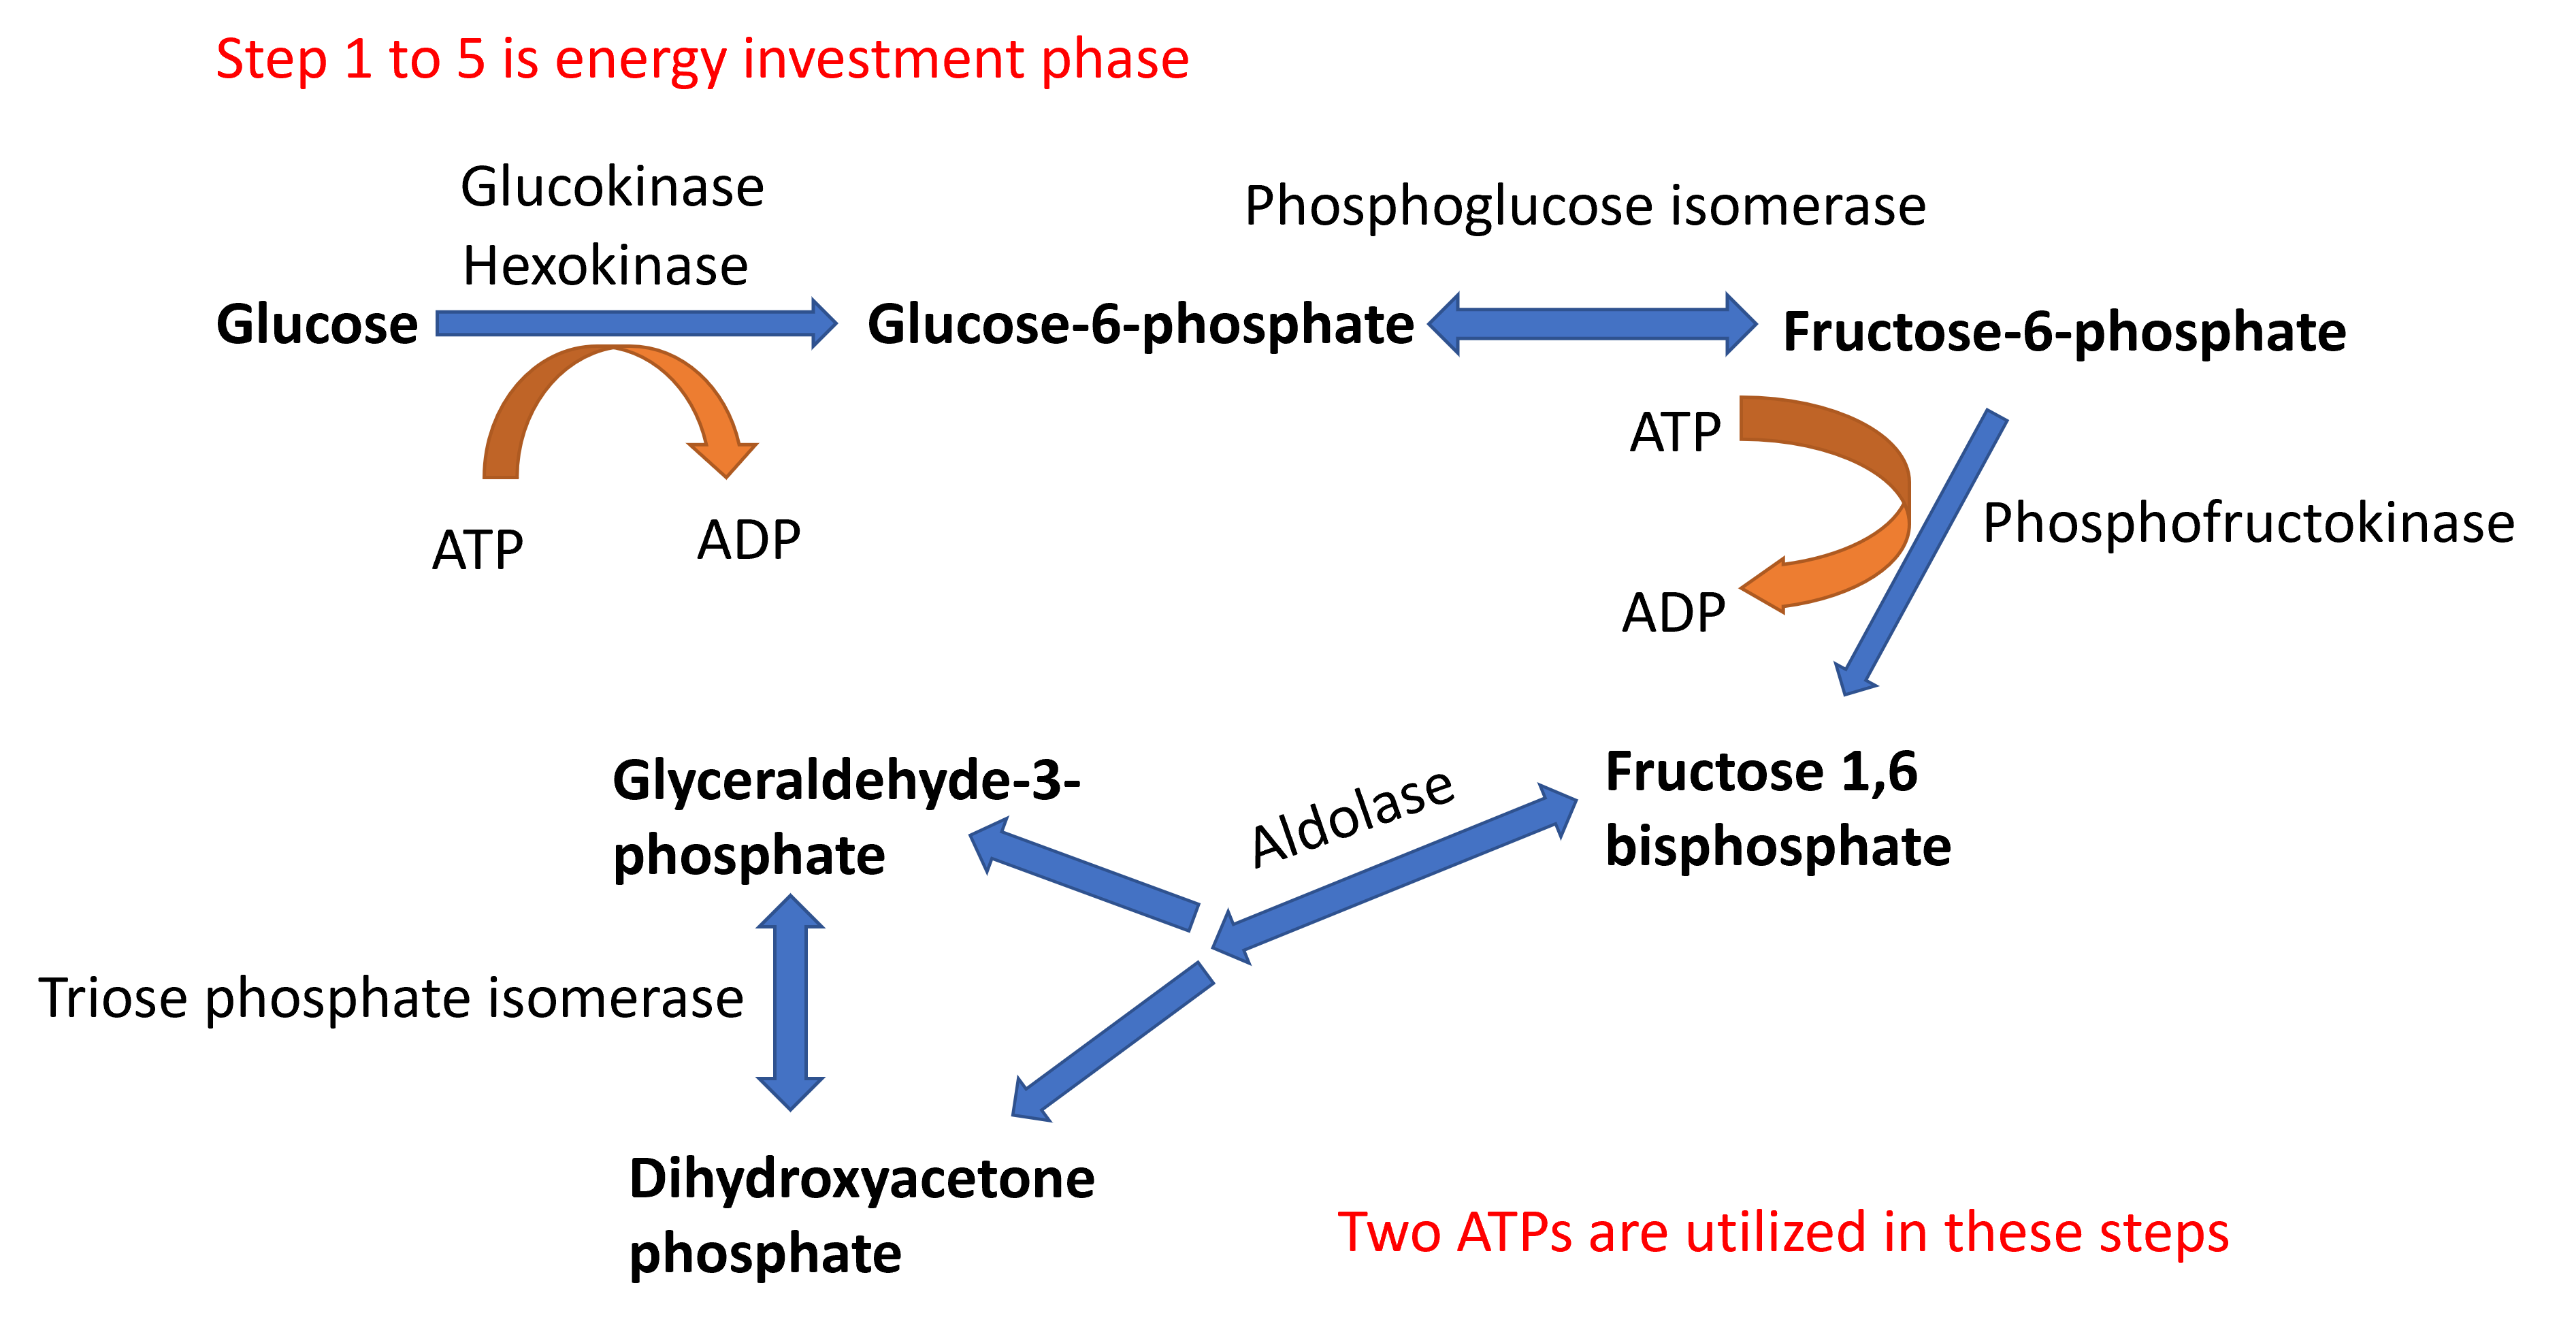
\includegraphics[width=\textwidth,height=4.16667in]{Images/Gly1.png}
\caption{Glycolysis phase 1}
\end{figure}

In the next phase, glyceraldehyde-3 phosphate is oxidized with reduction of NAD\^{}+ to NADH and substrate level phosphorylation at two steps to produce 4 ATPs per glyceraldehyde-3 phosphate.

\begin{figure}
\centering
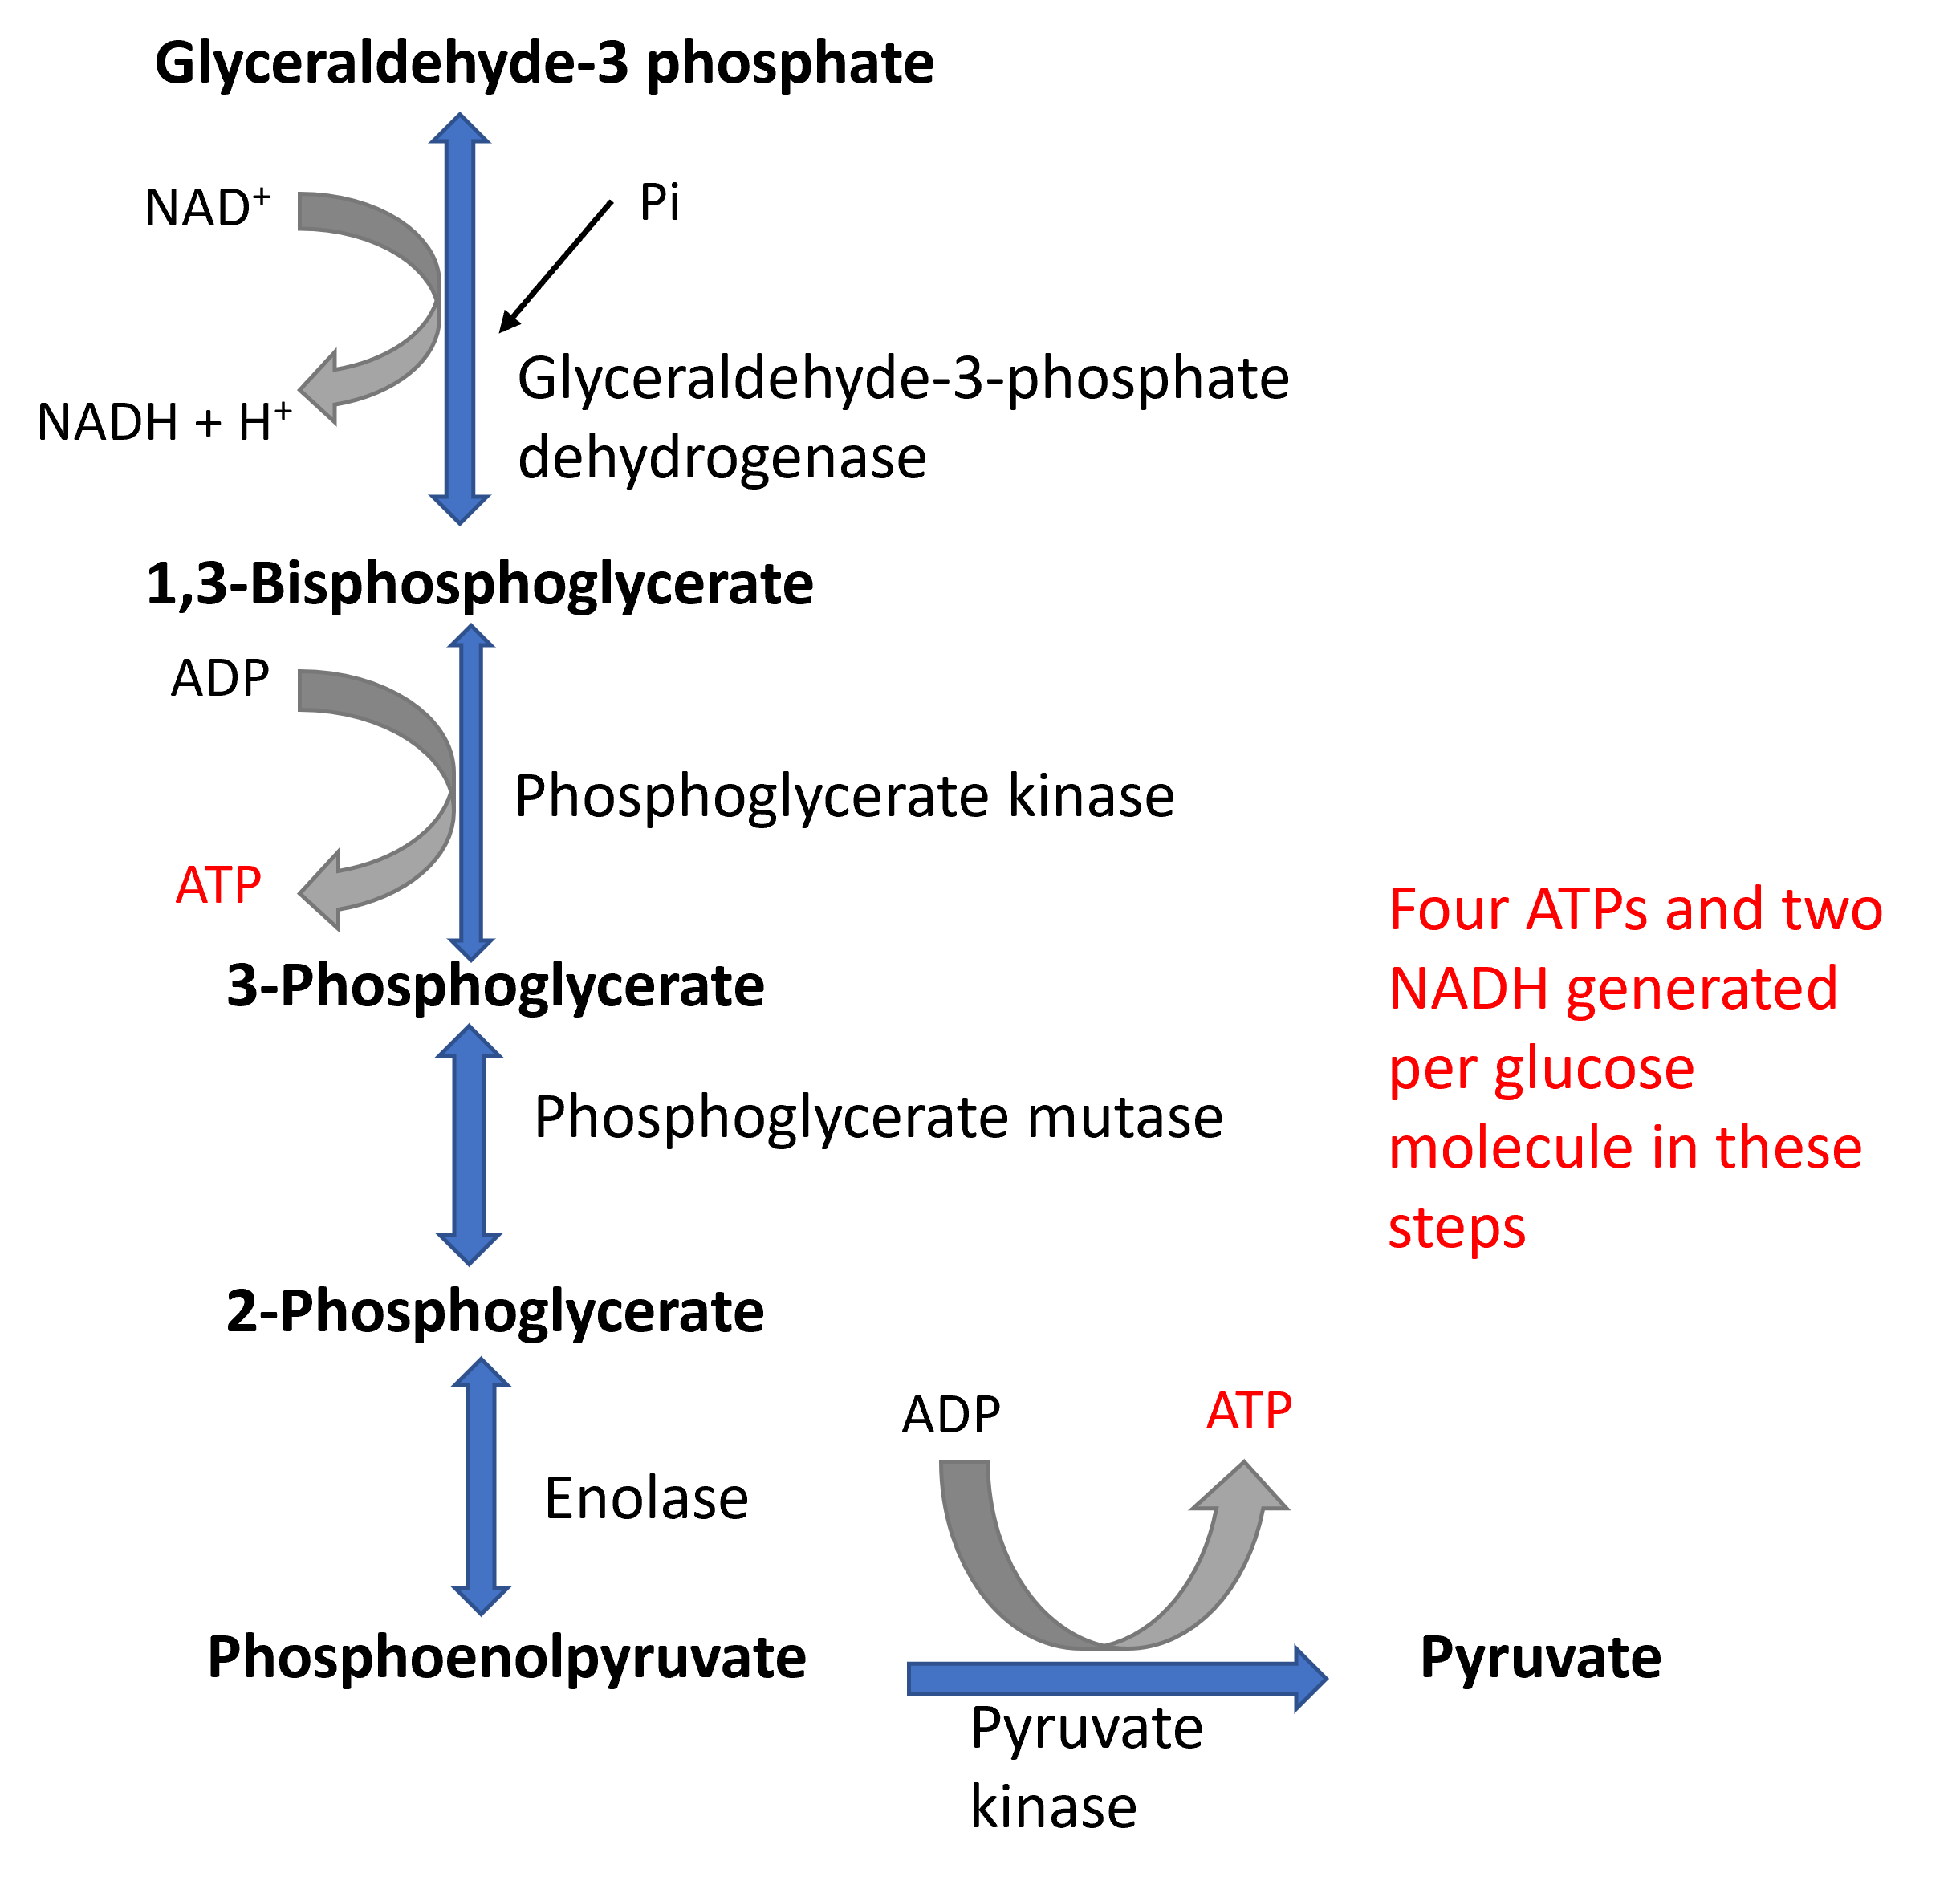
\includegraphics[width=\textwidth,height=4.16667in]{Images/Gly2.png}
\caption{Glycolysis phase 2}
\end{figure}

\subsection{Aerobic glycolysis}\label{aerobic-glycolysis}

Pyruvate is the end product of aerobic glycolysis. Pyruvate is further oxidized to acetyl-CoA and acetyl-CoA is oxidised in TCA cycle to reduce NAD\textsuperscript{+} and FAD to NADH and FADH\textsubscript{2}. NADH produced in glycolysis and TCA cycle is converted back to NAD\textsuperscript{+} in the process of oxidative phosphorylation (which produces ATP in presence of oxygen). Regeneration of NAD\textsuperscript{+} is necessary to sustain glycolysis.

\begin{figure}
\centering
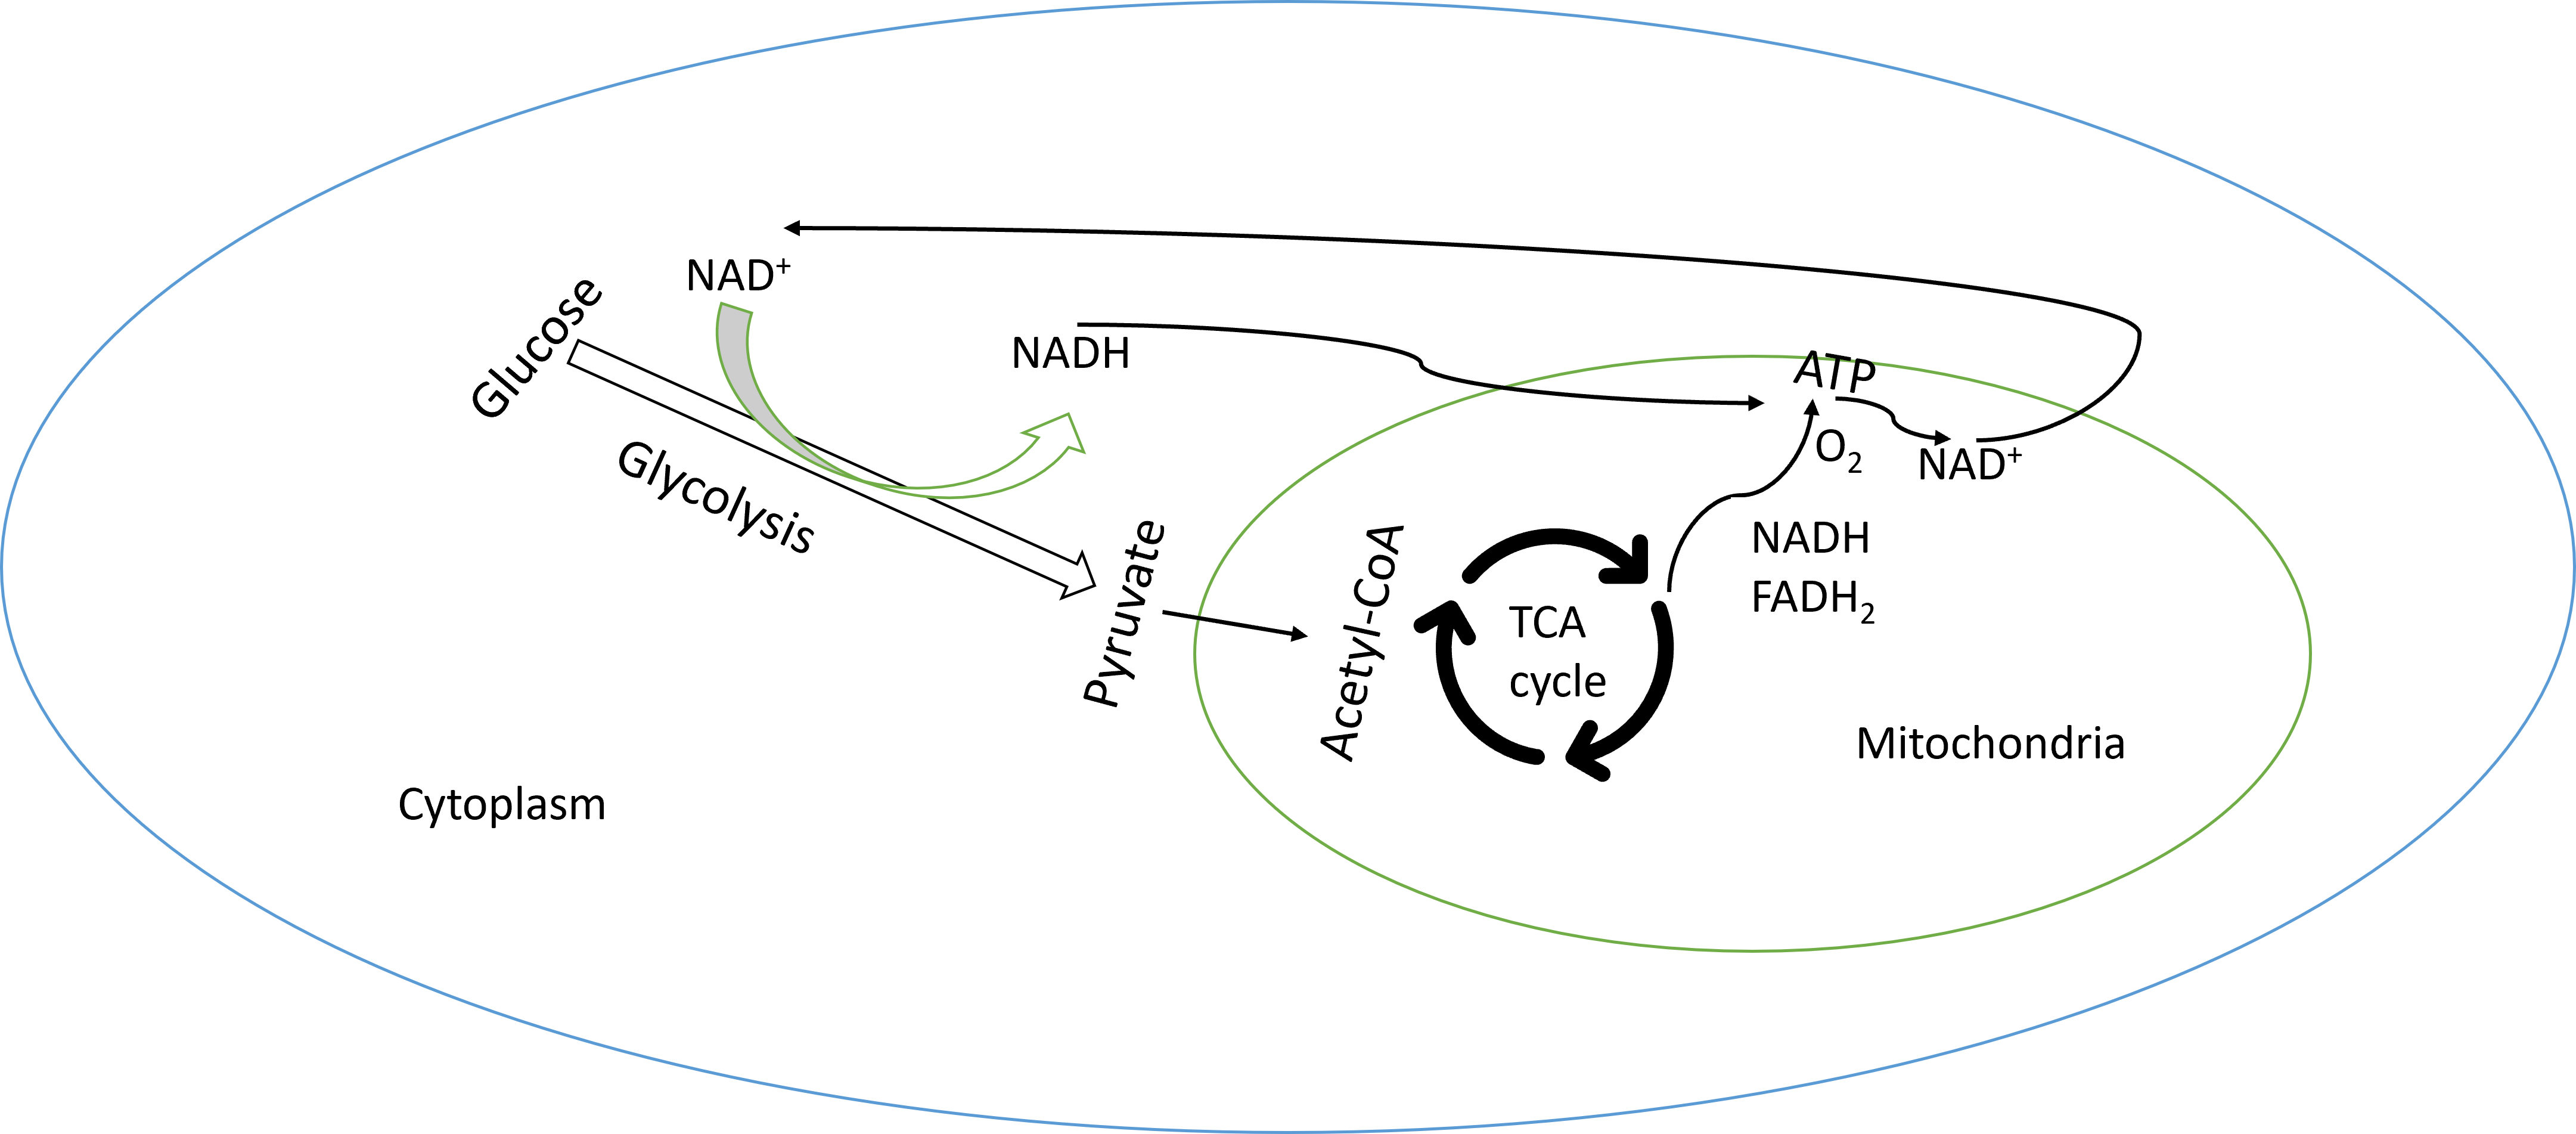
\includegraphics[width=\textwidth,height=2.08333in]{Images/AerobicGlycolysis.png}
\caption{Aerobic glycolysis}
\end{figure}

\subsection{Anaerobic glycolysis}\label{anaerobic-glycolysis}

In the absence of oxygen as in the case of muscle during sternous exercise or hypoxia due to reduced blood supply to tissues or in cells that lack mitochondria such as RBCs, the oxidation of NADH through oxidative phosphorylation does not take place. However, to produce ATP even in the absence of oxygen or mitochondria, NADH is oxidized to NAD\^{}+ with the help of reduction of pyruvate to lactate.

\begin{figure}
\centering
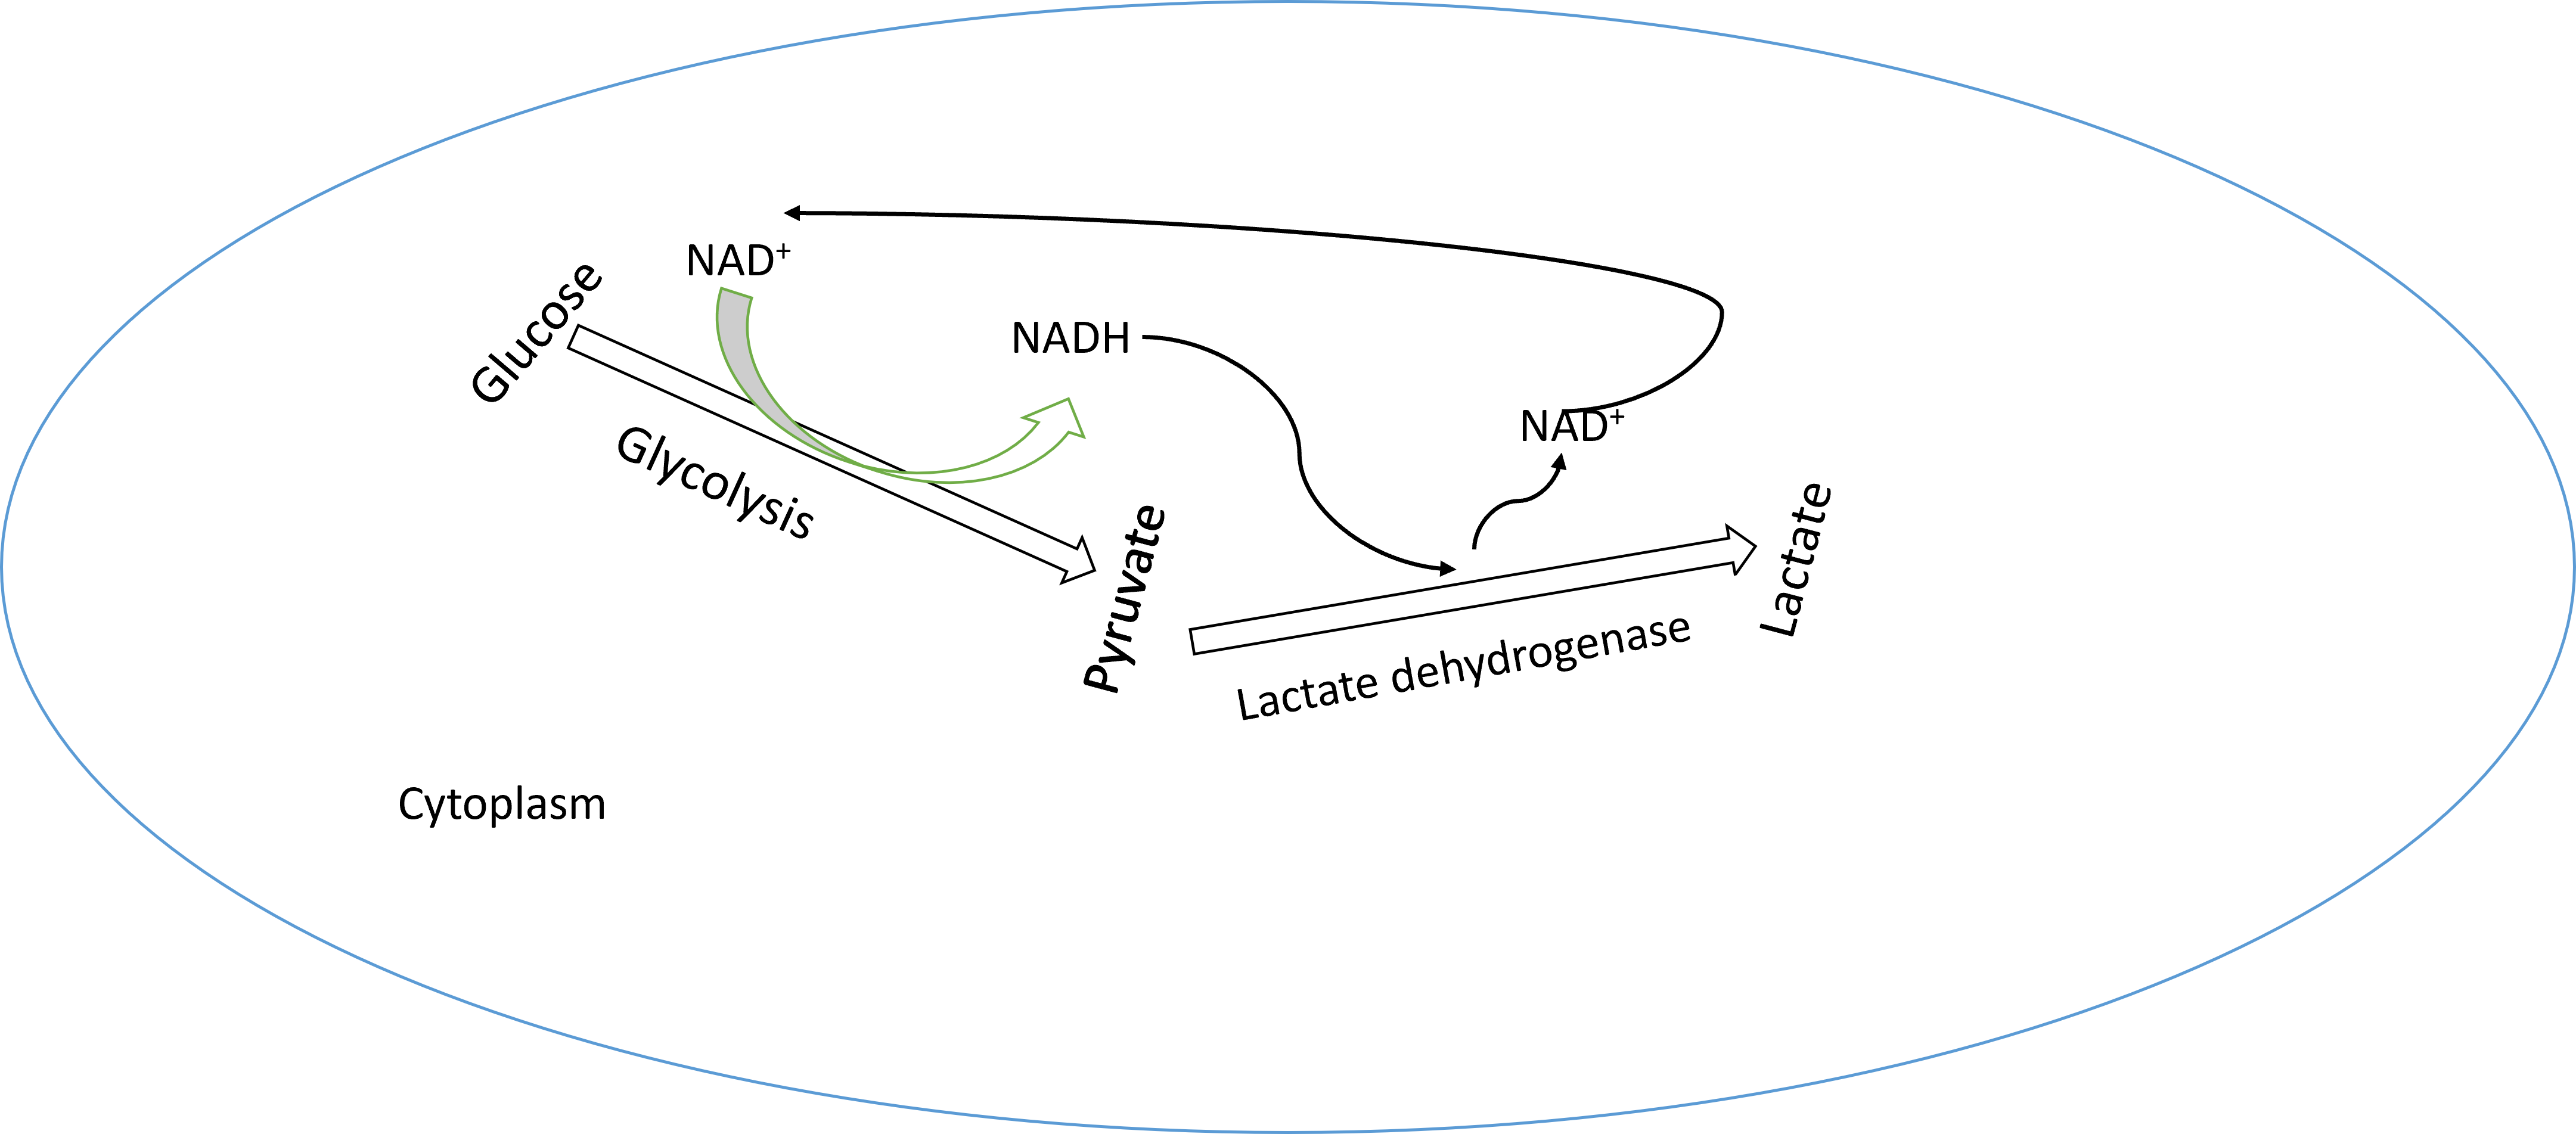
\includegraphics[width=\textwidth,height=2.08333in]{Images/AnaerobicGlycolysis.png}
\caption{Anaerobic glycolysis}
\end{figure}

\subsection{Energetics of glycolysis}\label{energetics-of-glycolysis}

Aerobic glycolysis produces 2 net ATPs and 2 NADH during the conversion of glucose to pyruvate. However, the complete oxidation of glucose to 6 carbon dioxide through further oxidation of pyruvate and TCA cycle produces a total of 32 molecules of ATP per glucose molecule.

Anaerobic glycolysis on the other hand will produce only 2 ATP per glucose molecule.

\subsection{Regulation of glycolysis}\label{regulation-of-glycolysis}

Phosphofructokinase (PFK-1) is the rate limiting enzyme of glycolysis. PFK-1 is inhibited allosterically when there is an increase in energy levels (indicated by ATP and citrate levels) and activated allosterically when there is decrease in energy levels (AMP).

PFK-1 is also regulated bby fructose 2,6 bisphosphate (Fr 2,6 BP), an allosteric activator. \hyperref[regulation-of-glycolysis-and-gluconeogenesis]{Levels of Fructose 2,6 bisphosphate are regulated by Insulin and Glucagon}.

\subsection{2,3 Bisphosphoglycerate pathway/Rapaport- Luebering shunt}\label{bisphosphoglycerate-pathwayrapaport--luebering-shunt}

This pathway is active only in RBCs and it involves production of 2,3 Bisphosphoglycerate from 1,3 Bisphosphoglycerate. 2,3 BPG binds to haemoglobin in RBCs and decreases its affinity to oxygen. 2,3 BPG favours release of oxygen from haemoglobin to tissues. Hypoxic conditions increases the production of 2,3 BPG helping the RBCs to deliver oxygen efficiently.

\subsection{Glycolysis inhibitor for blood collection}\label{glycolysis-inhibitor-for-blood-collection}

Sodium fluoride is an inhibitor of the enzyme enolase and this is added to blood samples collected for glucose estimation to stop consumption of glucose via glycolysis.

\section{Practice exercises}\label{practice-exercises-1}

\begin{enumerate}
\def\labelenumi{\arabic{enumi}.}
\tightlist
\item
  Glycolysis is regulated by allosteric modification of the enzyme
\end{enumerate}

\begin{itemize}
\tightlist
\item
  \begin{enumerate}
  \def\labelenumi{(\Alph{enumi})}
  \tightlist
  \item
    Enolase\\
  \end{enumerate}
\item
  \begin{enumerate}
  \def\labelenumi{(\Alph{enumi})}
  \setcounter{enumi}{1}
  \tightlist
  \item
    Aldolase\\
  \end{enumerate}
\item
  \begin{enumerate}
  \def\labelenumi{(\Alph{enumi})}
  \setcounter{enumi}{2}
  \tightlist
  \item
    Phosphofructokinase\\
  \end{enumerate}
\item
  \begin{enumerate}
  \def\labelenumi{(\Alph{enumi})}
  \setcounter{enumi}{3}
  \tightlist
  \item
    Lactate dehydrogenase
  \end{enumerate}
\end{itemize}

\begin{enumerate}
\def\labelenumi{\arabic{enumi}.}
\setcounter{enumi}{1}
\item
  The main function of glycolysis is to produce energy: TRUE / FALSE
\item
  In Anerobic glycolysis, NADH is reoxidized to NAD by
\end{enumerate}

\begin{itemize}
\tightlist
\item
  \begin{enumerate}
  \def\labelenumi{(\Alph{enumi})}
  \tightlist
  \item
    TCA cycle\\
  \end{enumerate}
\item
  \begin{enumerate}
  \def\labelenumi{(\Alph{enumi})}
  \setcounter{enumi}{1}
  \tightlist
  \item
    Oxidative phosphorylation\\
  \end{enumerate}
\item
  \begin{enumerate}
  \def\labelenumi{(\Alph{enumi})}
  \setcounter{enumi}{2}
  \tightlist
  \item
    Phosphofructokinase\\
  \end{enumerate}
\item
  \begin{enumerate}
  \def\labelenumi{(\Alph{enumi})}
  \setcounter{enumi}{3}
  \tightlist
  \item
    Lactate dehydrogenase
  \end{enumerate}
\end{itemize}

\begin{enumerate}
\def\labelenumi{\arabic{enumi}.}
\setcounter{enumi}{3}
\tightlist
\item
  RBCs depends on which of the following pathway for it's energy needs?
\end{enumerate}

\begin{itemize}
\tightlist
\item
  \begin{enumerate}
  \def\labelenumi{(\Alph{enumi})}
  \tightlist
  \item
    TCA cycle\\
  \end{enumerate}
\item
  \begin{enumerate}
  \def\labelenumi{(\Alph{enumi})}
  \setcounter{enumi}{1}
  \tightlist
  \item
    Oxidative phosphorylation\\
  \end{enumerate}
\item
  \begin{enumerate}
  \def\labelenumi{(\Alph{enumi})}
  \setcounter{enumi}{2}
  \tightlist
  \item
    Glycolysis\\
  \end{enumerate}
\item
  \begin{enumerate}
  \def\labelenumi{(\Alph{enumi})}
  \setcounter{enumi}{3}
  \tightlist
  \item
    Oxidation of fatty acids
  \end{enumerate}
\end{itemize}

\chapter{TCA cycle}\label{tca-cycle}

\section{Oxidation of pyruvate to acetyl-CoA}\label{oxidation-of-pyruvate-to-acetyl-coa}

Pyruvate is oxidized to acetyl-CoA by the enzyme pyruvate dehydrogenase. Pyruvate dehydrogenase is a multienzyme complex with copies of three enzymes --E1, E2, and E3. Pyruvate dehydrogenase requires the co-enzymes thiamine, lipoic acid, CoA, FAD, and NAD for its function. The overall reaction is oxidative decarboxylation of pyruvate to acetyl-CoA with release of carbon dioxide and reduction of NAD\textsuperscript{+} to NADH. The whole process happens in mitochondria after pyruvate is transported into mitochondria.

\section{Citric acid cycle}\label{citric-acid-cycle}

Citric acid cycle is the final metabolic pathway that produces energy from carbohydrates, proteins, and lipids. Citric acid cycle occurs only in aerobic conditions. Other names for the cycle are Kreb's cycle, and the tricarboxylic acid (TCA) cycle. It is a series of 8 chemical reactions in mitochondria that generates energy by complete oxidation of acetyl-CoA to two carbon dioxide molecules while reducing 3 NAD\textsuperscript{+} and 1 FADH\textsubscript{2}. The reaction starts with consumption of oxaloacetate and ends with regeneration of oxaloacetate. Thus oxaloacetate is technically a catalyst for the TCA cycyle and is required only in small concentration.

\begin{figure}
\centering
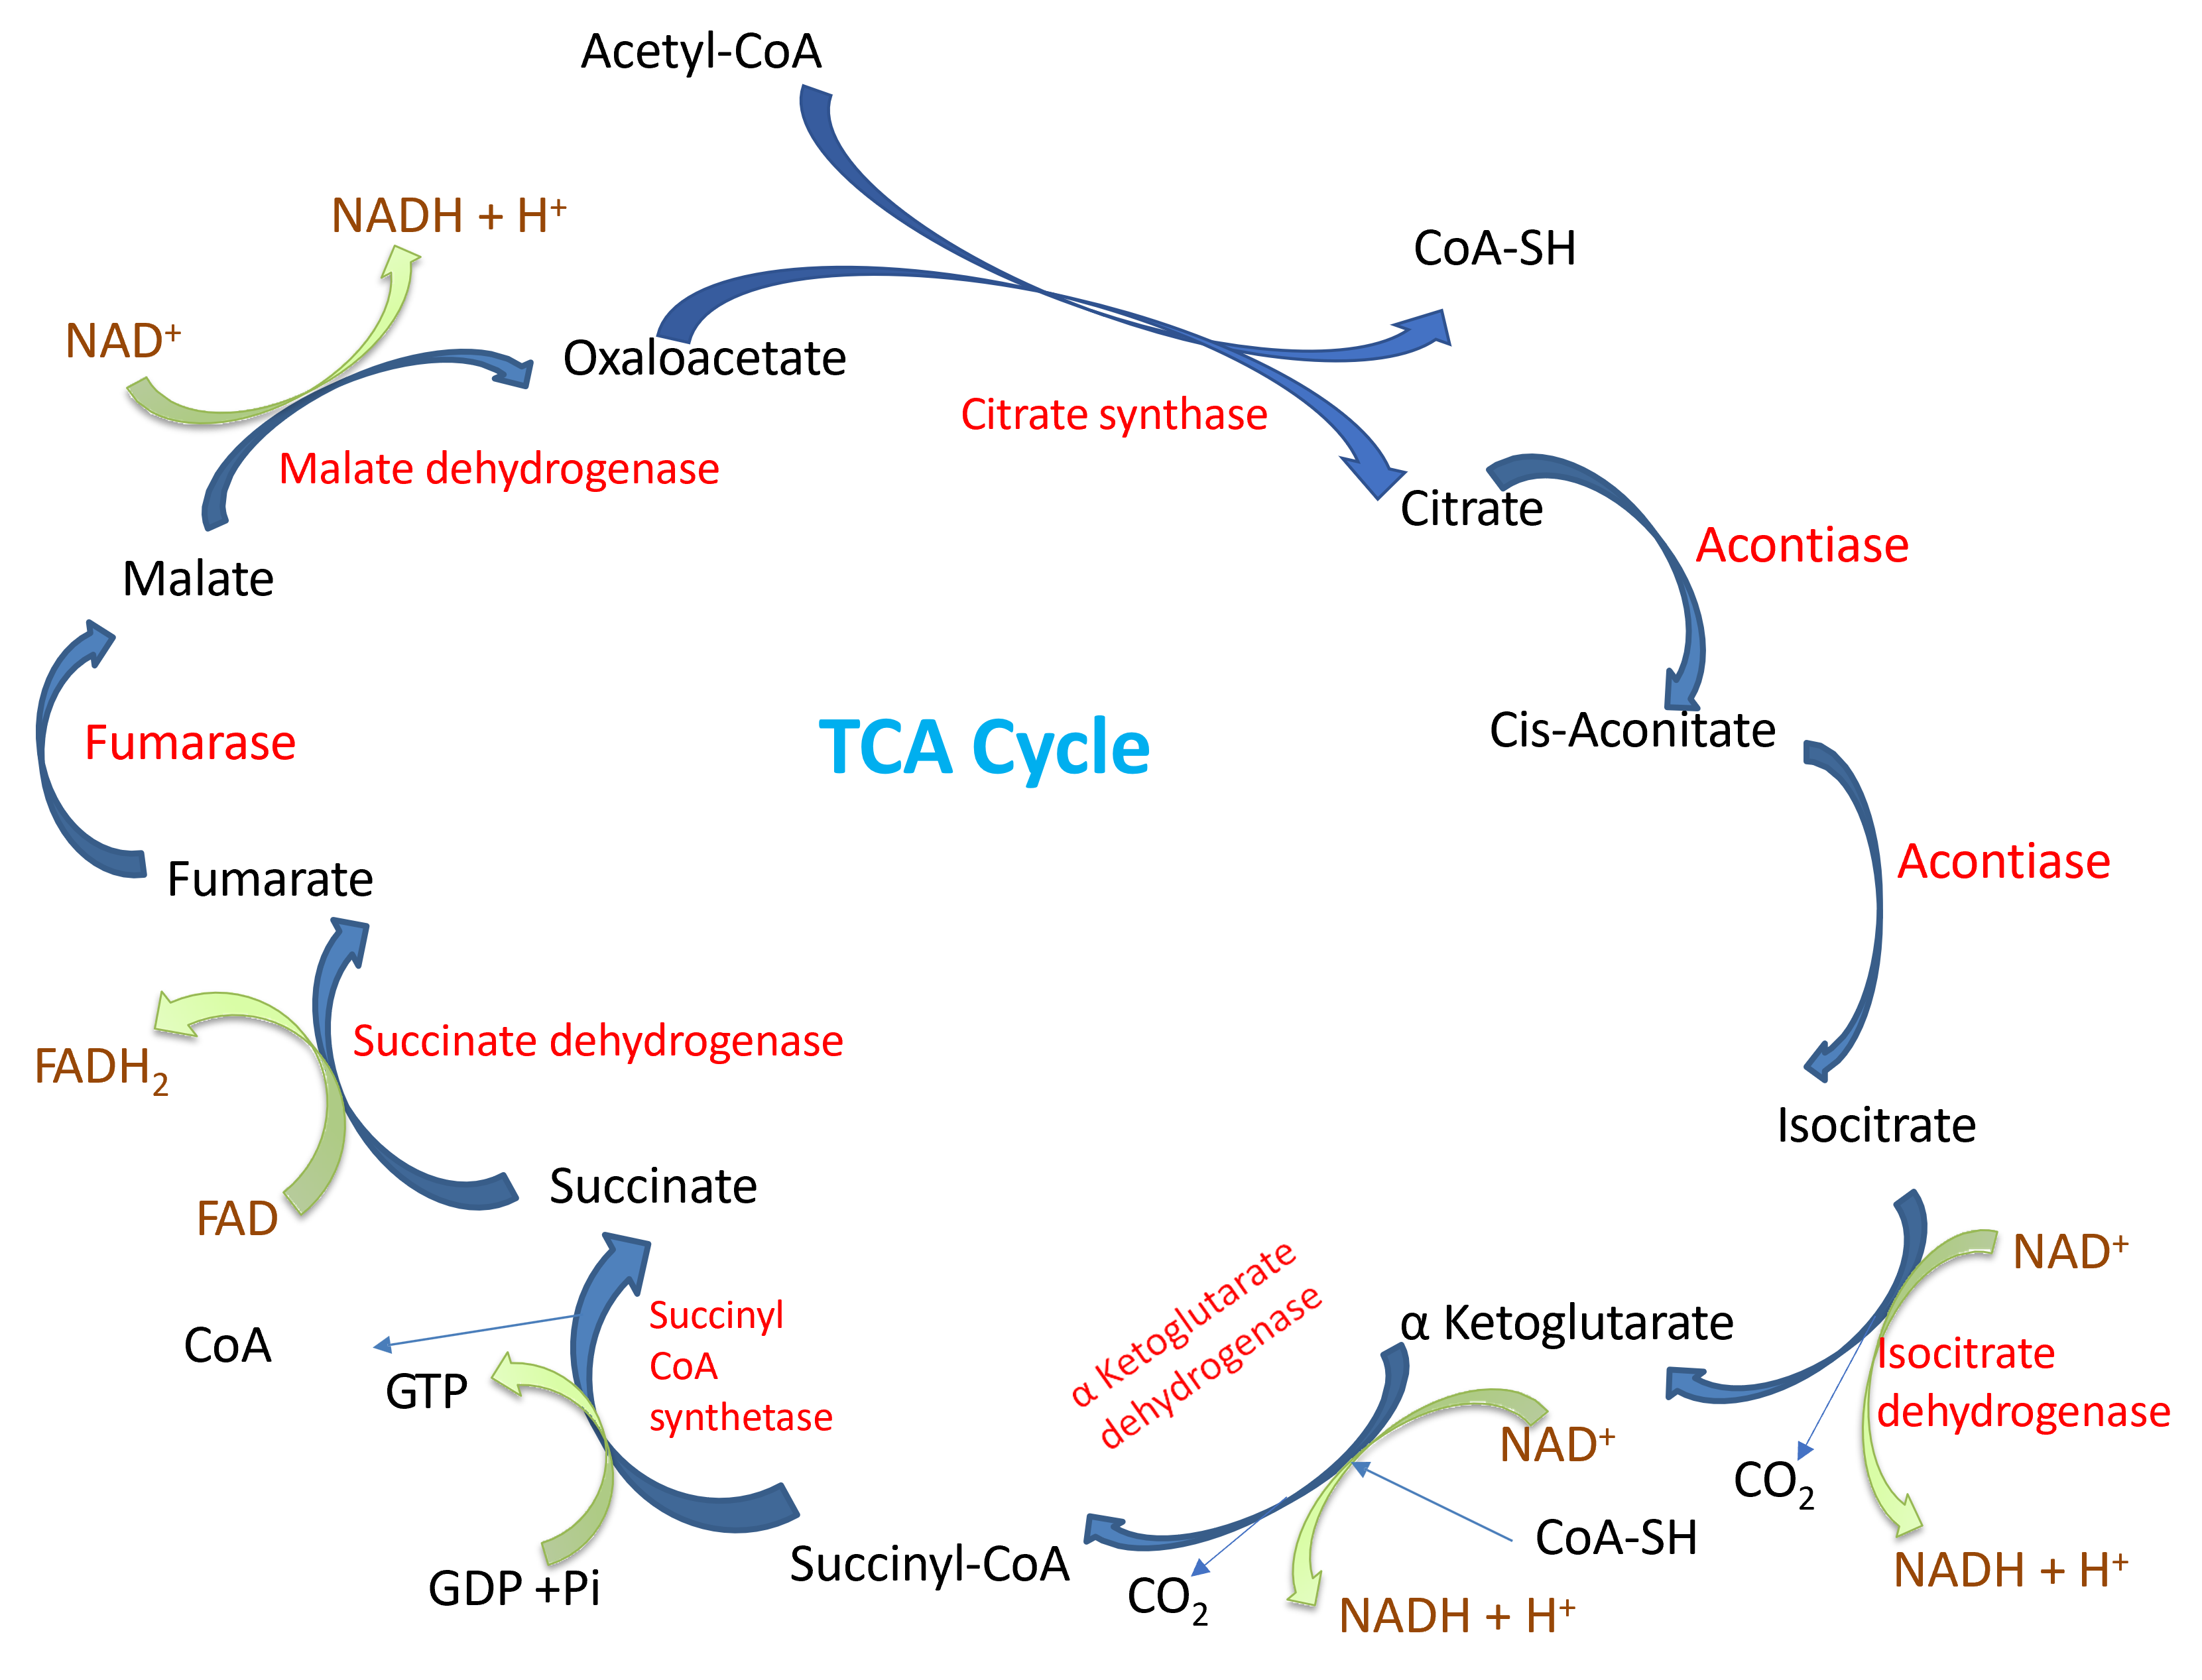
\includegraphics[width=\textwidth,height=5.20833in]{Images/TCA.png}
\caption{TCA cyle}
\end{figure}

Each turn of the cycle reduces 3 NAD\textsuperscript{+} to 3 NADH and 1 FADH to 1 FADH\textsubscript{2} molecules along with substrate level phosphorylation to produce a GTP. Each NADH is capable of producing 2.5 ATPs, and each FADH\textsubscript{2} is capable of producing 1.5 ATPs. Thus each turn of the cycle produces 10 ATPs (2.5 * 3 NADH + 1.5 * 1 FADH\textsubscript{2} + 1 ATP (= 1 GTP)).

\section{Amphibolic pathway}\label{amphibolic-pathway}

Citric acid cycle is an amphibolic pathway i.e., it has both anabolic and catabolic functions. It is catabolic since it is the final oxidation pathway for carbohydrates, proteins, and lipids which prodduces ATP. It is anabolic because intermediate molecules in the citric acid cycle are used as sources of carbons for synthesis of glucose, amino acids, fatty acids, heme, and nucleotides. Anabolic reactions that consume TCA cycle intermediates are also called cataplerotic reactions. Reactions that replenish TCA cycle intermediates to sustain TCA cycle are called anaplerotic reactions. Glucogenic amino acids replenish TCA cyle intermediates in anaplerotic reactions.

\section{Regulation of TCA cycle}\label{regulation-of-tca-cycle}

TCA cycle is regulated at the level of formation of acetyl-CoA from pyruvate. Energy status of the cell and availability of reducing equivalents determine the rate of oxidation of pyruvate to acetyl-CoA.

The enzymes citrate synthase (release of CoA from Acetyl-CoA), isocitrate dehydrogenase (oxidation and release of CO\textsubscript{2}), and alpha-ketoglutarate dehydrogenase (oxidation and release of CO\textsubscript{2}) catalyze reactions that release large free energy and is regulated by energy level (ATP to AMP ratio) and reducing equivalents (NADH to NAD\textsuperscript{+} ratio) and are also regulated allosterically by their products.

\section{Practice exercises}\label{practice-exercises-2}

\begin{enumerate}
\def\labelenumi{\arabic{enumi}.}
\tightlist
\item
  The reactions that replenish intermediates of TCA cycle are called
\end{enumerate}

\begin{itemize}
\tightlist
\item
  \begin{enumerate}
  \def\labelenumi{(\Alph{enumi})}
  \tightlist
  \item
    Anabolic reactions\\
  \end{enumerate}
\item
  \begin{enumerate}
  \def\labelenumi{(\Alph{enumi})}
  \setcounter{enumi}{1}
  \tightlist
  \item
    Amphibolic reactions\\
  \end{enumerate}
\item
  \begin{enumerate}
  \def\labelenumi{(\Alph{enumi})}
  \setcounter{enumi}{2}
  \tightlist
  \item
    Catabolic reactions\\
  \end{enumerate}
\item
  \begin{enumerate}
  \def\labelenumi{(\Alph{enumi})}
  \setcounter{enumi}{3}
  \tightlist
  \item
    Anaplerotic reactions
  \end{enumerate}
\end{itemize}

\chapter{Glycogen metabolism}\label{glycogen-metabolism}

\section{Importance of glycogen metabolism}\label{importance-of-glycogen-metabolism}

During fasting, blood glucose is maintained by release of glucose from liver. Liver releases glucose by breaking down the stored glycogen into glucose units.Liver glycogen acts as the major source of blood glucose during fasting. In muscle, glycogen supplies glucose during exercise. Muscle doesn't release glucose into blood. During fed state (after eating food), glycogen stores must be replenished by synthesising glycogen from glucose.

\section{Glycogenesis}\label{glycogenesis}

Glycogenesis is the synthesis of glycogen from glucose during fed state in liver, and during resting state in muscle. The pathway take place in cytoplasm.

Glucose should be activated by conjugation to UDP to take part in glycogenesis. UDP-Glucose is produced by reaction of UTP with glucose-1 phosphate. Glucose-1 phosphate is produced by phosphorylation of glucose to glucose-6 phosphate and then isomerism to glucose-1 phosphate.

Glycogen synthase catalyzes the formation of α (1 to 4) glycosidic bonds between glucose molecules to form glycogen, however it cannot use a free glucose molecule as an acceptor and can only catalyse α (1 to 4) glycosidic bond formation on a pre-existing chain of glucose molecules (primer). In absence of a primer, a protein called glycogenin adds at least 4 molecules of glucose to itself forming a primer. Glycogen synthase subsequently elongates the primer by adding glucose molecules and forming α (1 to 4) glycosidic bond them.

After sufficient elongation of the chain, a branching enzyme with 4 to 6 transferas activity cleaves a short segment of the chain by breaking a α (1 to 4) glycosidic bond and forming a α (1 to 6) glycosidic bond at a deeper point on the chain forming a branch. Elongation and branching repeats itself till the formation of the highly branched structure of glycogen.

Glycogenesis

\section{Glycogenolysis}\label{glycogenolysis}

Glycogenolysis is the process of breakdown of glycogen into glucose. It occurs during fasting in liver and exercise in muscle. The enzyme glycogen phosphorylase sequentially removes glucose from glycogen as glucose-1 phosphate with the help of inorganic phosphate from the ends of the glycogen molecule resulting in formation of dextrin. The debranching enzyme with α (1 to 4) to α (1 to 4) glucantransferase activity, removes chain of glucose molecules from the branches and reattaches them to the end of linear chains. The glucose molecule at the branching point with α (1 to 6) glycosidic bond is removed by α (1 to 6) glucosidase activity of the debranching enzyme. Repeated action by glycogen phosphorylase and debranching enzyme results in release of glucose-1 phosphate. Glucose-1 phosphate is converted to glucose-6 phosphate. In the liver, glucose-6 phosphate is converted to glucose by glucose-6 phosphatase and release into the blood. Muscle lacks this enzyme and thus glucose-6 phosphate is used for glycolysis and ATP production in the muscle during exercise.

Glycogenolysis

\section{Regulation of glycogen metabolism}\label{regulation-of-glycogen-metabolism}

Glycogenesis and glycogenolysis are tightly regulated.During well fed state, glycogen synthesis is increased in liver. During fasting, glycogenolysis is increased in liver.In muscle, glycogenolysis occurs during exercise and glycogenesis during rest.

Regulation occurs through allosteric regulators and covalent modification through hormonal regulation.

\subsection{Allsoteric regulation of glycogen metabolism}\label{allsoteric-regulation-of-glycogen-metabolism}

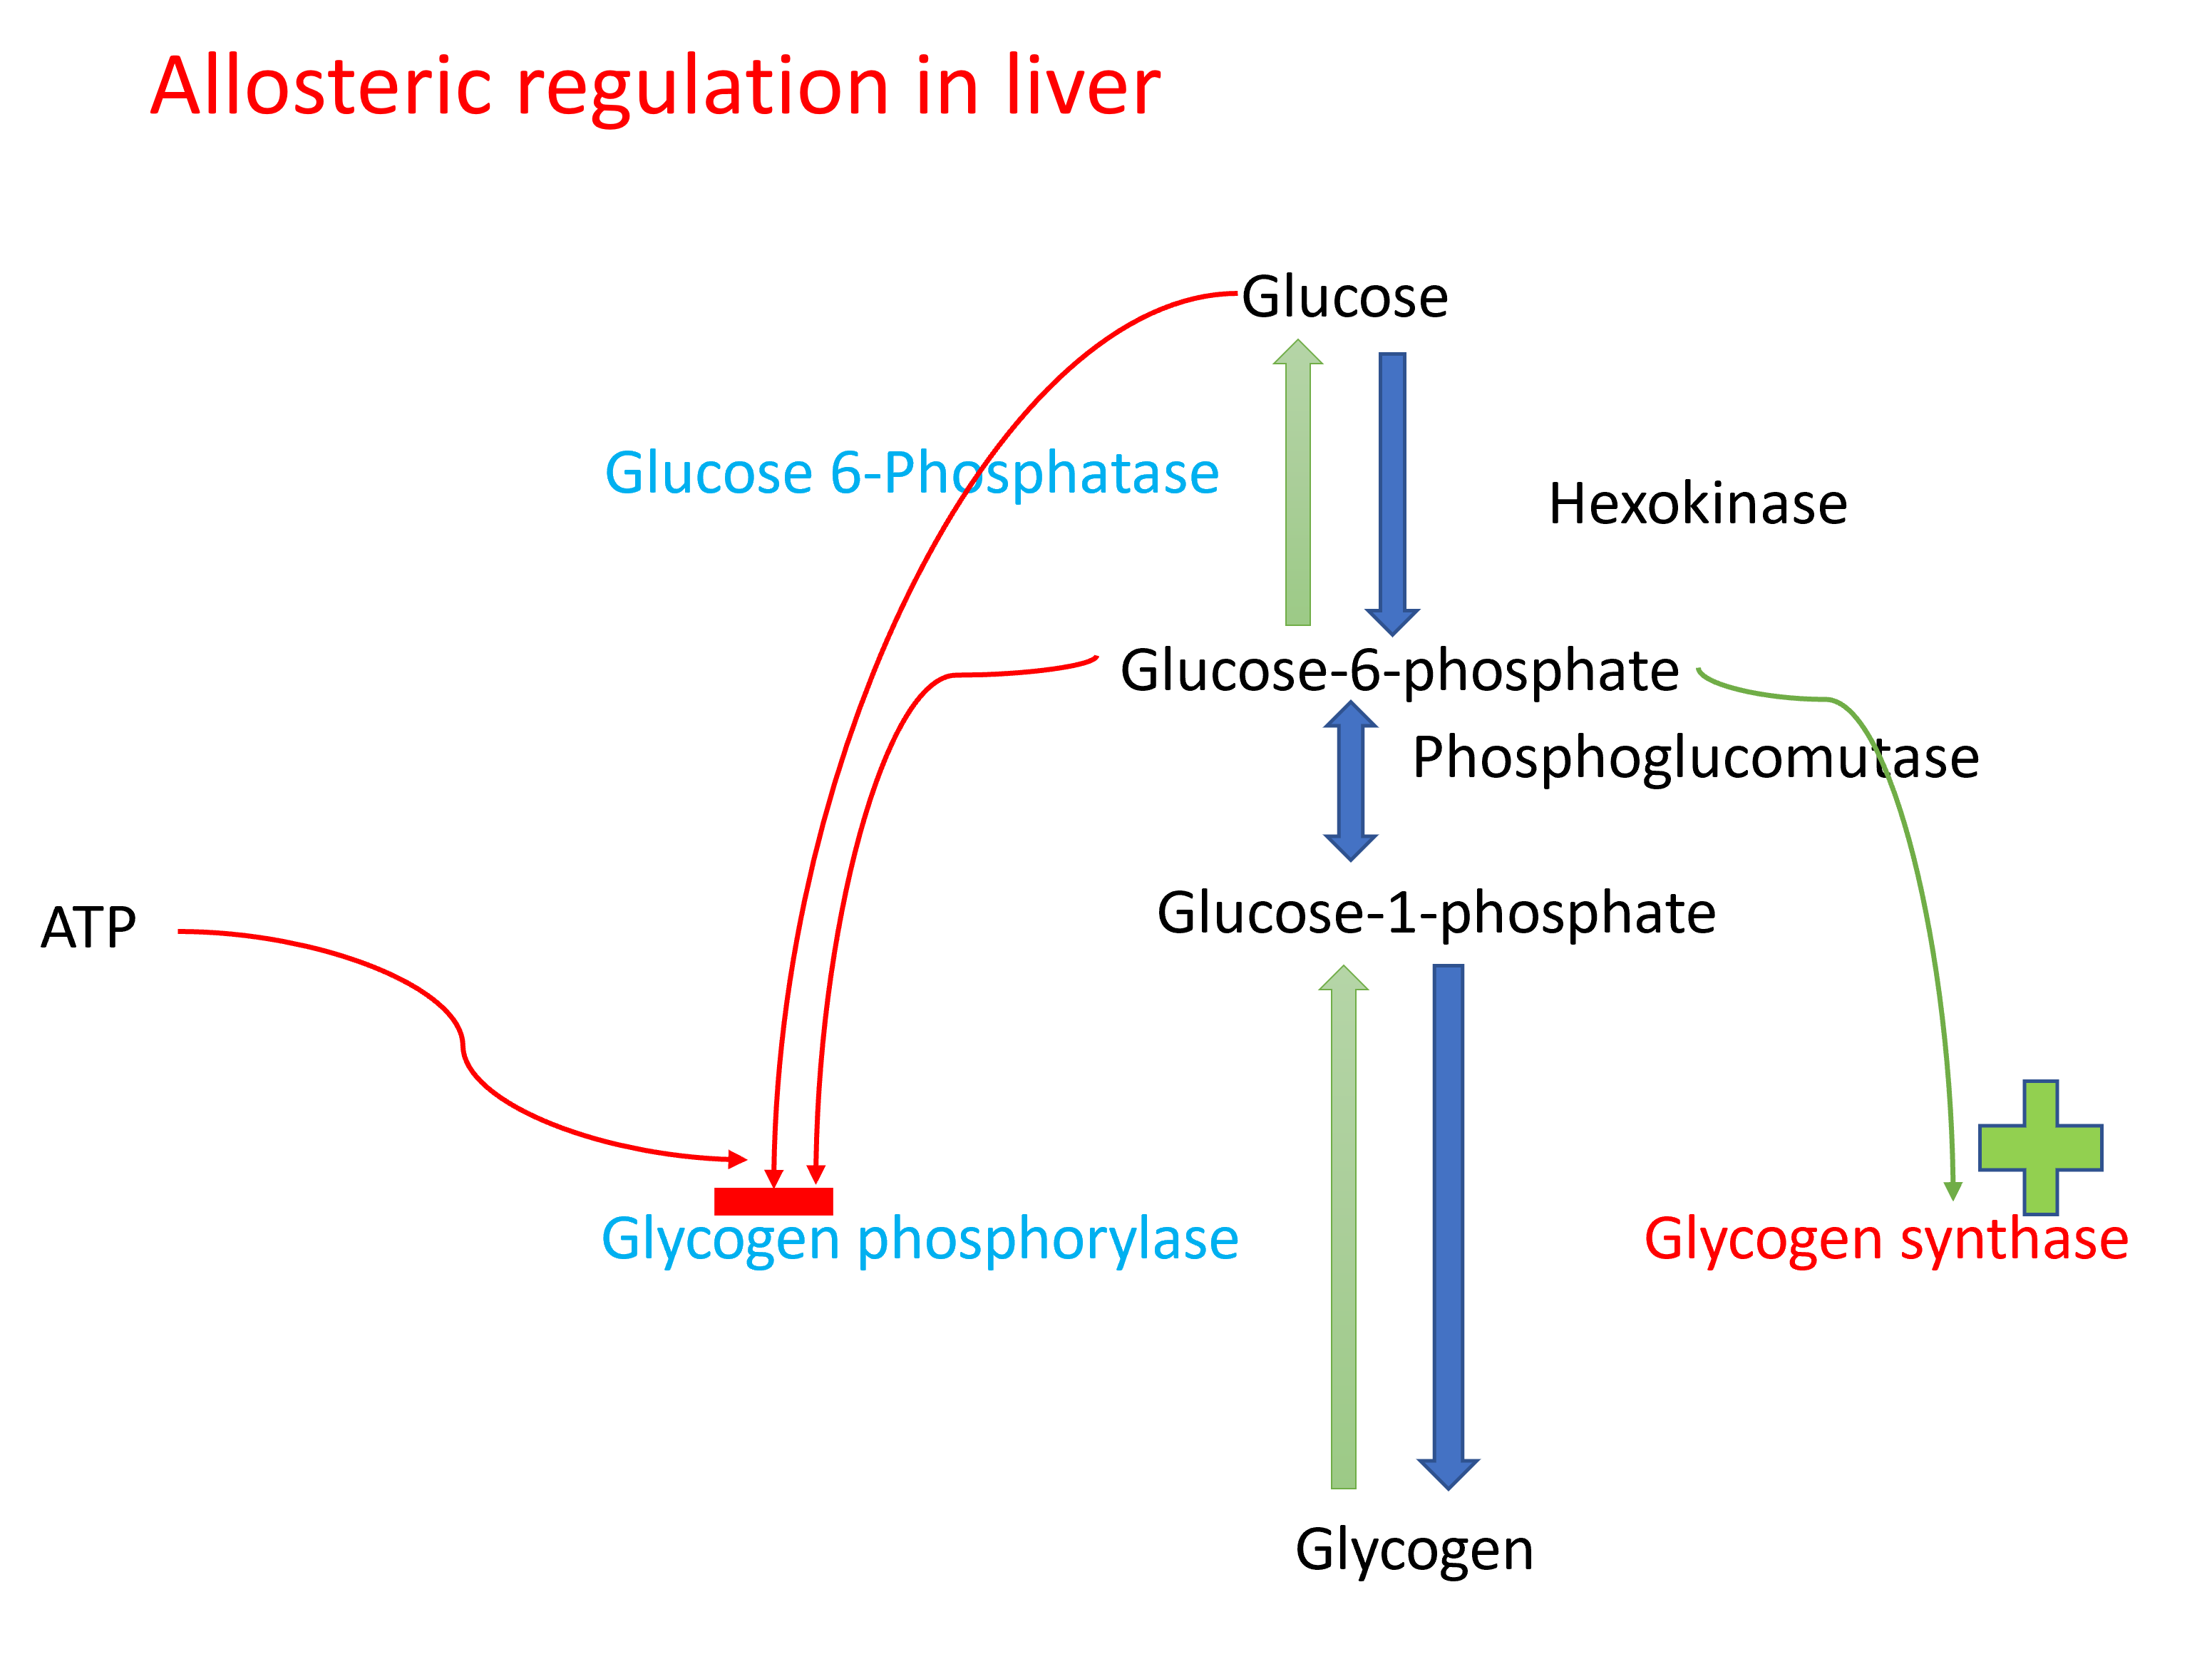
\includegraphics[width=0.5\textwidth,height=\textheight]{Images/Gly_allo_liver.png}

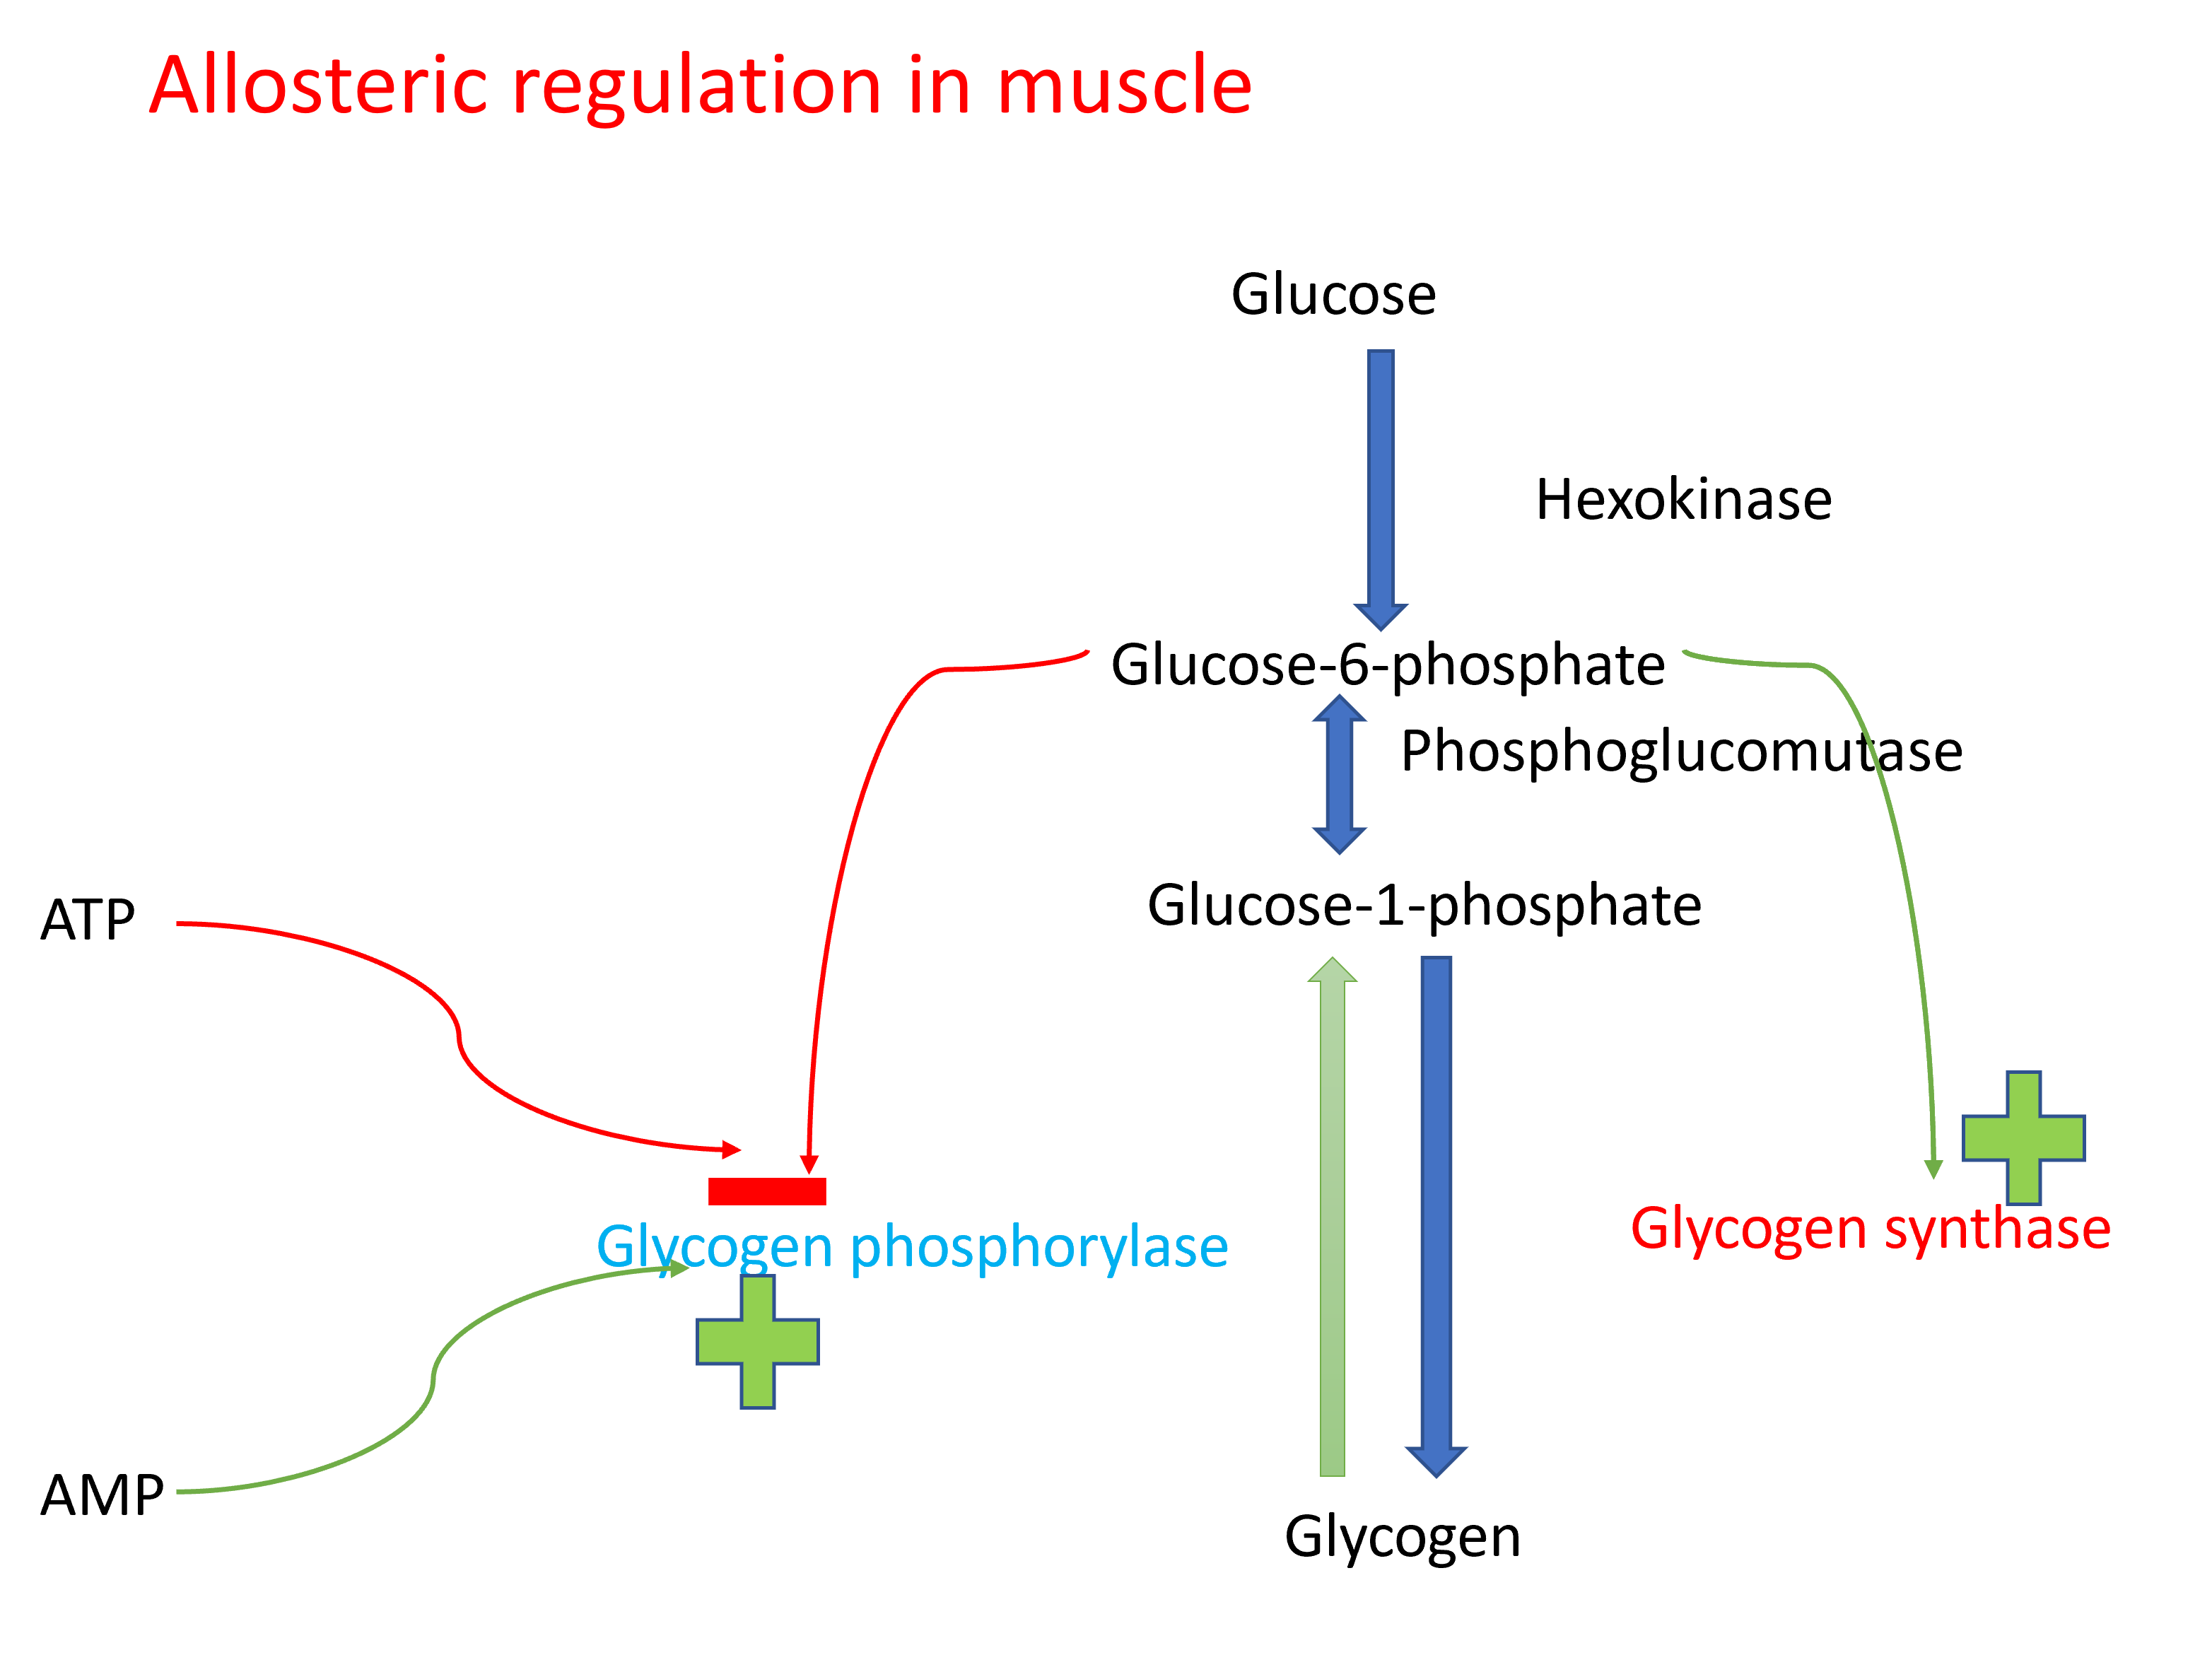
\includegraphics[width=0.5\textwidth,height=\textheight]{Images/Gly_allo_muscle.png}

\subsection{Hormonal regulation of glycogen metabolism}\label{hormonal-regulation-of-glycogen-metabolism}

Major hormones involved in regulation of glycogen metabolism are Insulin, glucagon, and epinephrine. Insulin increases glycogenesis and decreases glycogenolysis. This happens during well fed state.
During fasting, glucagon increases glycogenolysis and decreases glycogenesis in liver. Epinephrine increases glycogenolysis and decreases glycogenesis in liver and muscle.

Hormonal regulation of glycogenesis

Hormonal regulation of glycogenolysis

\subsection{Glycogen storage diseases}\label{glycogen-storage-diseases}

Glycogen storage diseases are a group of disorders with genetic defect in enzymes involved in synthesis or breakdown of glycogen. They are characterized by deposition of abnormal type or quantity of glycogen in tissues. Some of the glycogen storage diseases are Von Gierke's disease, Pompe's disease, Cori's disease, and McArdle's syndrome.

The clinical features of Glycogen storage diseases include hepatomegaly (enlargement of liver), hypoglycemia especially during fasting (glycogenolysis is impaired), enlargement of kidneys (renomegaly), chronic kidney disease, muscle -- weakness, and enlargement of heart (cardiomegaly).

\begin{longtable}[]{@{}
  >{\raggedright\arraybackslash}p{(\columnwidth - 4\tabcolsep) * \real{0.2353}}
  >{\raggedright\arraybackslash}p{(\columnwidth - 4\tabcolsep) * \real{0.4118}}
  >{\raggedright\arraybackslash}p{(\columnwidth - 4\tabcolsep) * \real{0.3529}}@{}}
\toprule\noalign{}
\begin{minipage}[b]{\linewidth}\raggedright
Type
\end{minipage} & \begin{minipage}[b]{\linewidth}\raggedright
Name of the disease
\end{minipage} & \begin{minipage}[b]{\linewidth}\raggedright
Enzyme involved
\end{minipage} \\
\midrule\noalign{}
\endhead
\bottomrule\noalign{}
\endlastfoot
Type 1 & Von Gierke disease & Glucose 6-phosphatase \\
Type 2 & Pompe disease & Lysosomal~ α (1 to 4) and α (1 to 6) glucosidase(acid maltase) \\
Type 3 & Limit dextrinosisForbe or Cori disease & Muscle debranching enzyme \\
Type 4 & Anderson disease & Branching enzyme \\
Type 5 & McArdle disease & Muscle phosphorylase \\
Type 6 & Hers disease & Liver phosphorylase \\
\end{longtable}

\section{Practice exercises}\label{practice-exercises-3}

\begin{enumerate}
\def\labelenumi{\arabic{enumi}.}
\tightlist
\item
  Muscle glycogen cannot contribute to the blood glucose because of the absence of which of the following enzyme in muscle?
\end{enumerate}

\begin{itemize}
\tightlist
\item
  \begin{enumerate}
  \def\labelenumi{(\Alph{enumi})}
  \tightlist
  \item
    Glucose 6-phosphatase\\
  \end{enumerate}
\item
  \begin{enumerate}
  \def\labelenumi{(\Alph{enumi})}
  \setcounter{enumi}{1}
  \tightlist
  \item
    Glucokinase\\
  \end{enumerate}
\item
  \begin{enumerate}
  \def\labelenumi{(\Alph{enumi})}
  \setcounter{enumi}{2}
  \tightlist
  \item
    Hexokinase\\
  \end{enumerate}
\item
  \begin{enumerate}
  \def\labelenumi{(\Alph{enumi})}
  \setcounter{enumi}{3}
  \tightlist
  \item
    Phosphoglucomutase
  \end{enumerate}
\end{itemize}

\begin{enumerate}
\def\labelenumi{\arabic{enumi}.}
\setcounter{enumi}{1}
\tightlist
\item
  Match the hormone with its effect on glycogen metabolism
\end{enumerate}

\begin{itemize}
\item
  ``Insulin:
\item
  \begin{enumerate}
  \def\labelenumi{(\Alph{enumi})}
  \tightlist
  \item
    Increased glycogenesis\\
  \end{enumerate}
\item
  \begin{enumerate}
  \def\labelenumi{(\Alph{enumi})}
  \setcounter{enumi}{1}
  \tightlist
  \item
    Increased glycogenolysis in muscle\\
  \end{enumerate}
\item
  \begin{enumerate}
  \def\labelenumi{(\Alph{enumi})}
  \setcounter{enumi}{2}
  \tightlist
  \item
    Increased gluconeogenesis
  \end{enumerate}
\end{itemize}

''

\begin{itemize}
\item
  ``Epinephrine:
\item
  \begin{enumerate}
  \def\labelenumi{(\Alph{enumi})}
  \tightlist
  \item
    Increased glycogenesis\\
  \end{enumerate}
\item
  \begin{enumerate}
  \def\labelenumi{(\Alph{enumi})}
  \setcounter{enumi}{1}
  \tightlist
  \item
    Increased glycogenolysis in muscle\\
  \end{enumerate}
\item
  \begin{enumerate}
  \def\labelenumi{(\Alph{enumi})}
  \setcounter{enumi}{2}
  \tightlist
  \item
    Increased gluconeogenesis
  \end{enumerate}
\end{itemize}

''

\begin{itemize}
\item
  ``Glucagon:
\item
  \begin{enumerate}
  \def\labelenumi{(\Alph{enumi})}
  \tightlist
  \item
    Increased glycogenesis\\
  \end{enumerate}
\item
  \begin{enumerate}
  \def\labelenumi{(\Alph{enumi})}
  \setcounter{enumi}{1}
  \tightlist
  \item
    Increased glycogenolysis in muscle\\
  \end{enumerate}
\item
  \begin{enumerate}
  \def\labelenumi{(\Alph{enumi})}
  \setcounter{enumi}{2}
  \tightlist
  \item
    Increased gluconeogenesis
  \end{enumerate}
\end{itemize}

''

\chapter{Gluconeogenesis}\label{gluconeogenesis}

Gluconeogenesis is the process of synthesis of glucose from non-carbohydrate sources such as lactate, glucogenic amino acids, glycerol, and propionyl Co-A. Gluconeogenesis occurs mostly in liver and to some extent in kidney. Gluconeogenesis maintains blood glucose levels during fasting and starvation.\\

Gluconeogenesis is not a simple reversal of glycolysis. Glycolysis is essentially irreversible (at physiological conditions of the cell) at three steps: phosphoenolpyruvate to pyruvate, fructose-6 phosphate to fructose-1,6 bisphosphate, and glucose to glucose-6 phosphate catalyzed by the enzymes hexokinase, phosphofructokinase, and Pyruvate kinase. In gluconeogenesis, these steps are by passed by 4 reactions catalyzed by different enzymes.\\

Pyruvate is converted to phosphoenolpyruvate by two reactions. First pyruvate is carboxylated to oxaloacetate in the mitochondria. Oxaloacetate cannot be transported out of mitochondria. It is reduced to malate and malate is transported from mitochondria to cytoplasm. This reaction oxidizes a NADH molecule to NAD\textsuperscript{+}. Malate is oxidized back to oxaloacetate in the cytoplasm which reduces NAD\textsuperscript{+} to NADH. Oxaloacetate is then converted to phosphoenol pyruvate by decarboxylation. In these reactions, reducing equivalents are effectively transported from mitochondria to cytoplasm which is crucial for gluconeogenesis. These reactions also consume two ATP equivalents per pyruvate to phosphoenolpyruvate generation while the opposite reaction generates only one ATP.\\

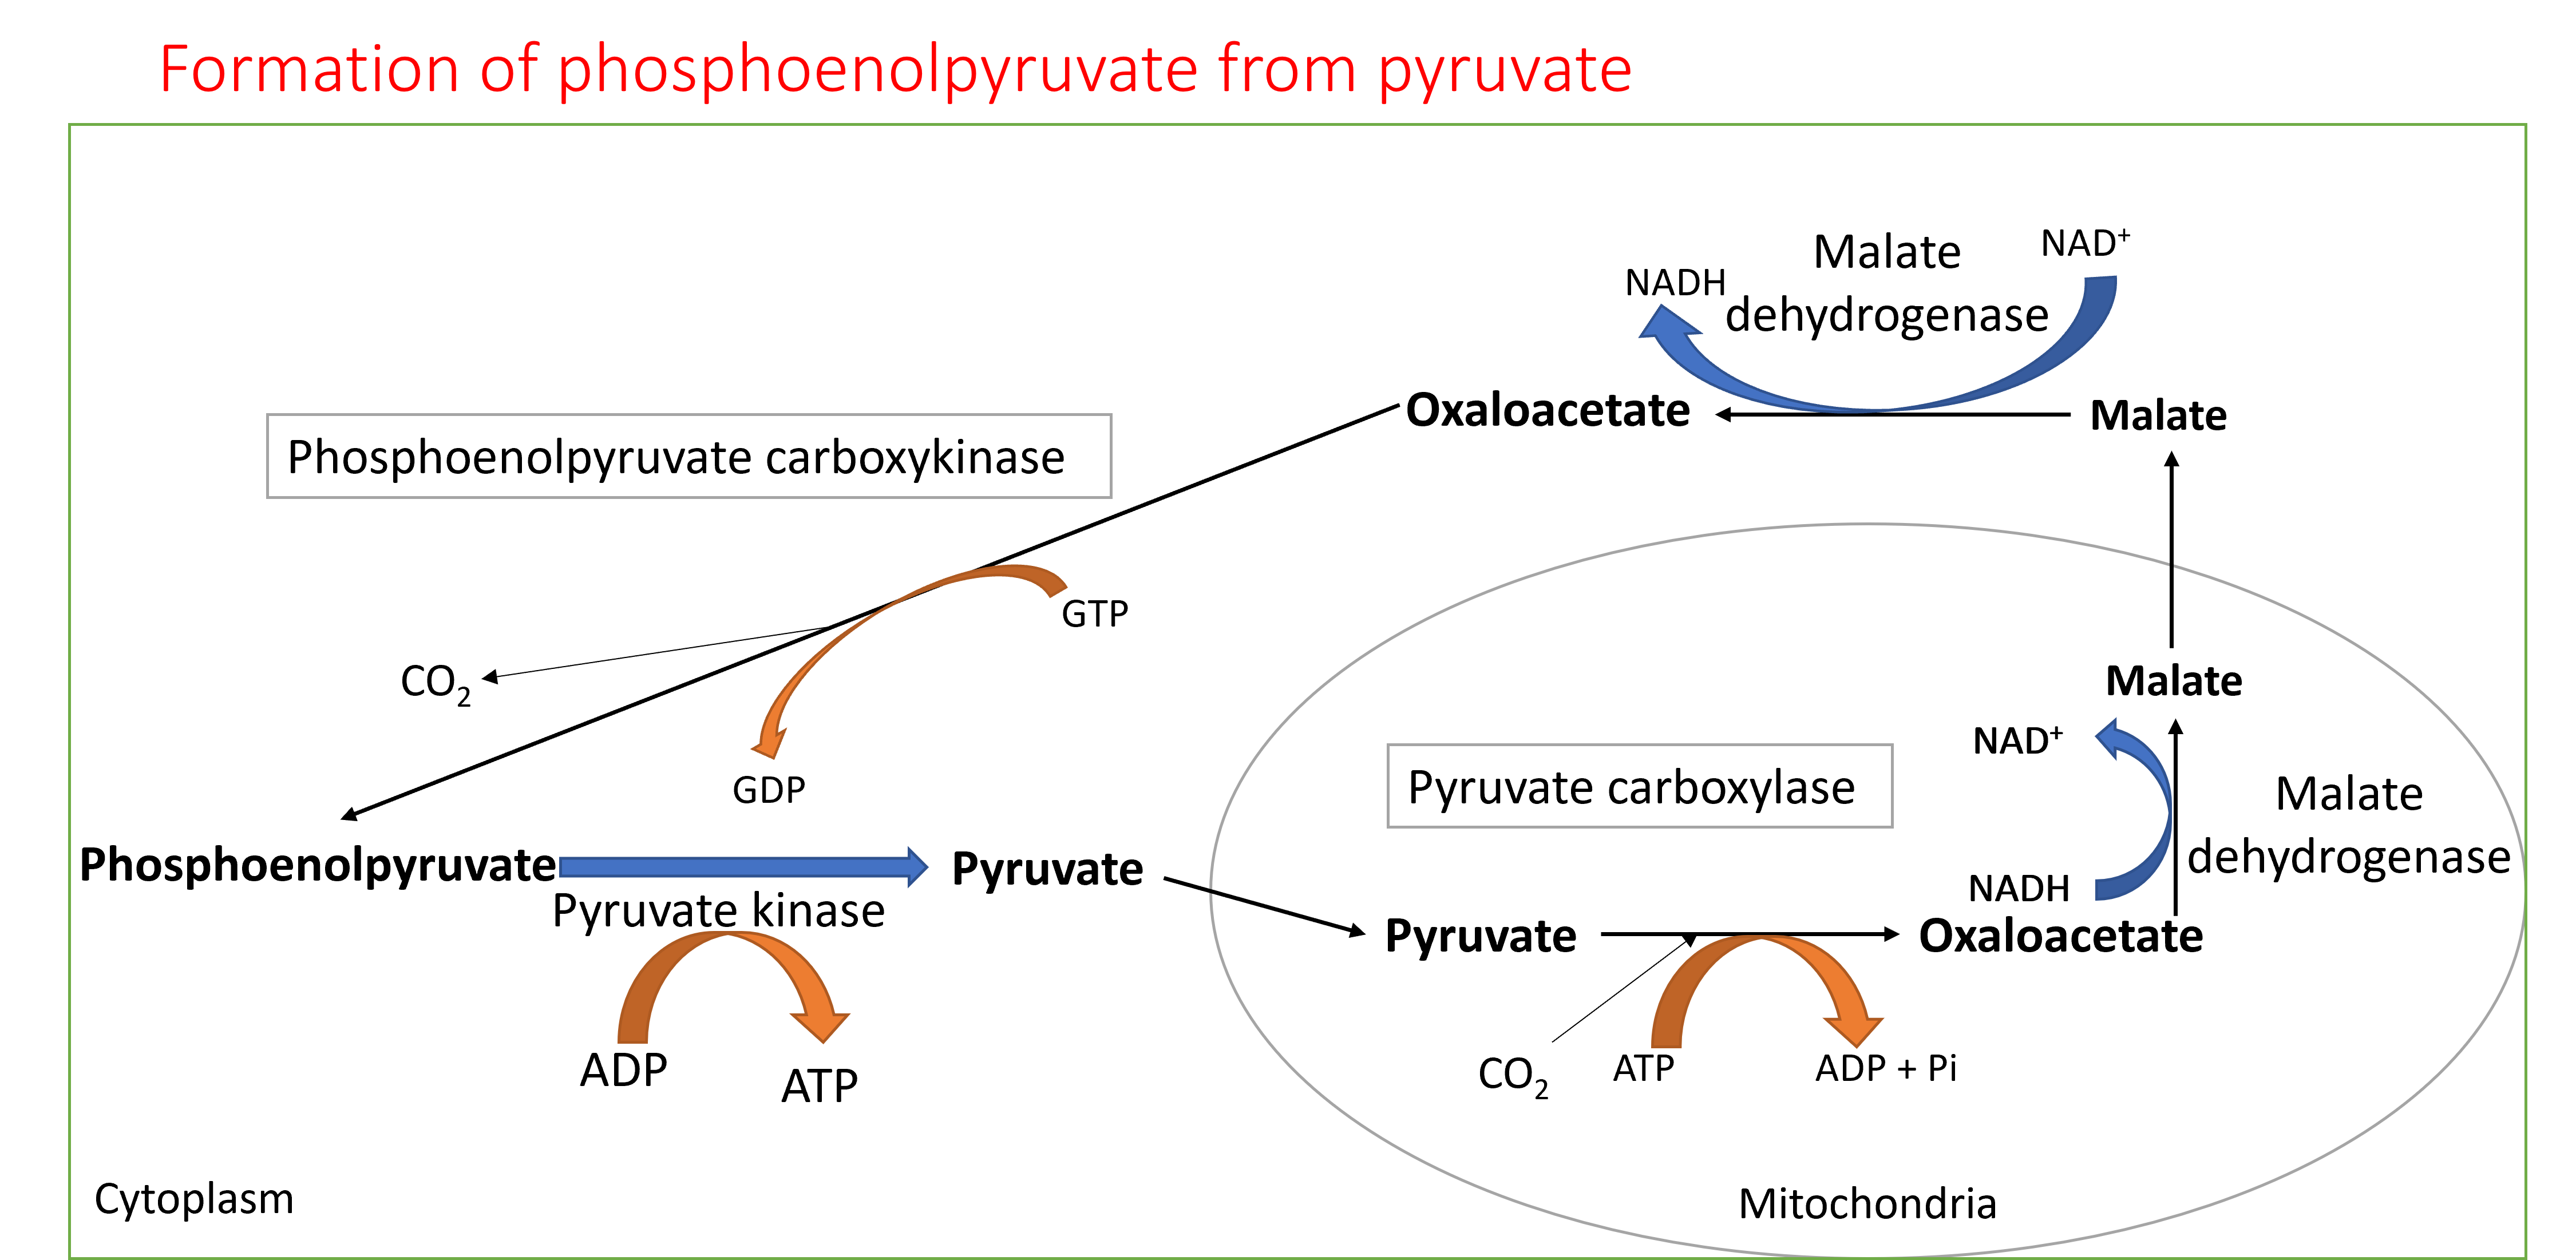
\includegraphics[width=\textwidth,height=3.125in]{Images/pep.png}

Frucose-1,6 bisphosphate is converted to fructose-6 phosphate by the enzyme fructose-1,6 bisphophatase with the release of inorganic phosphate, and glucose-6 phosphate is converted to glucose by the enzyme glucose-6 phosphatase.

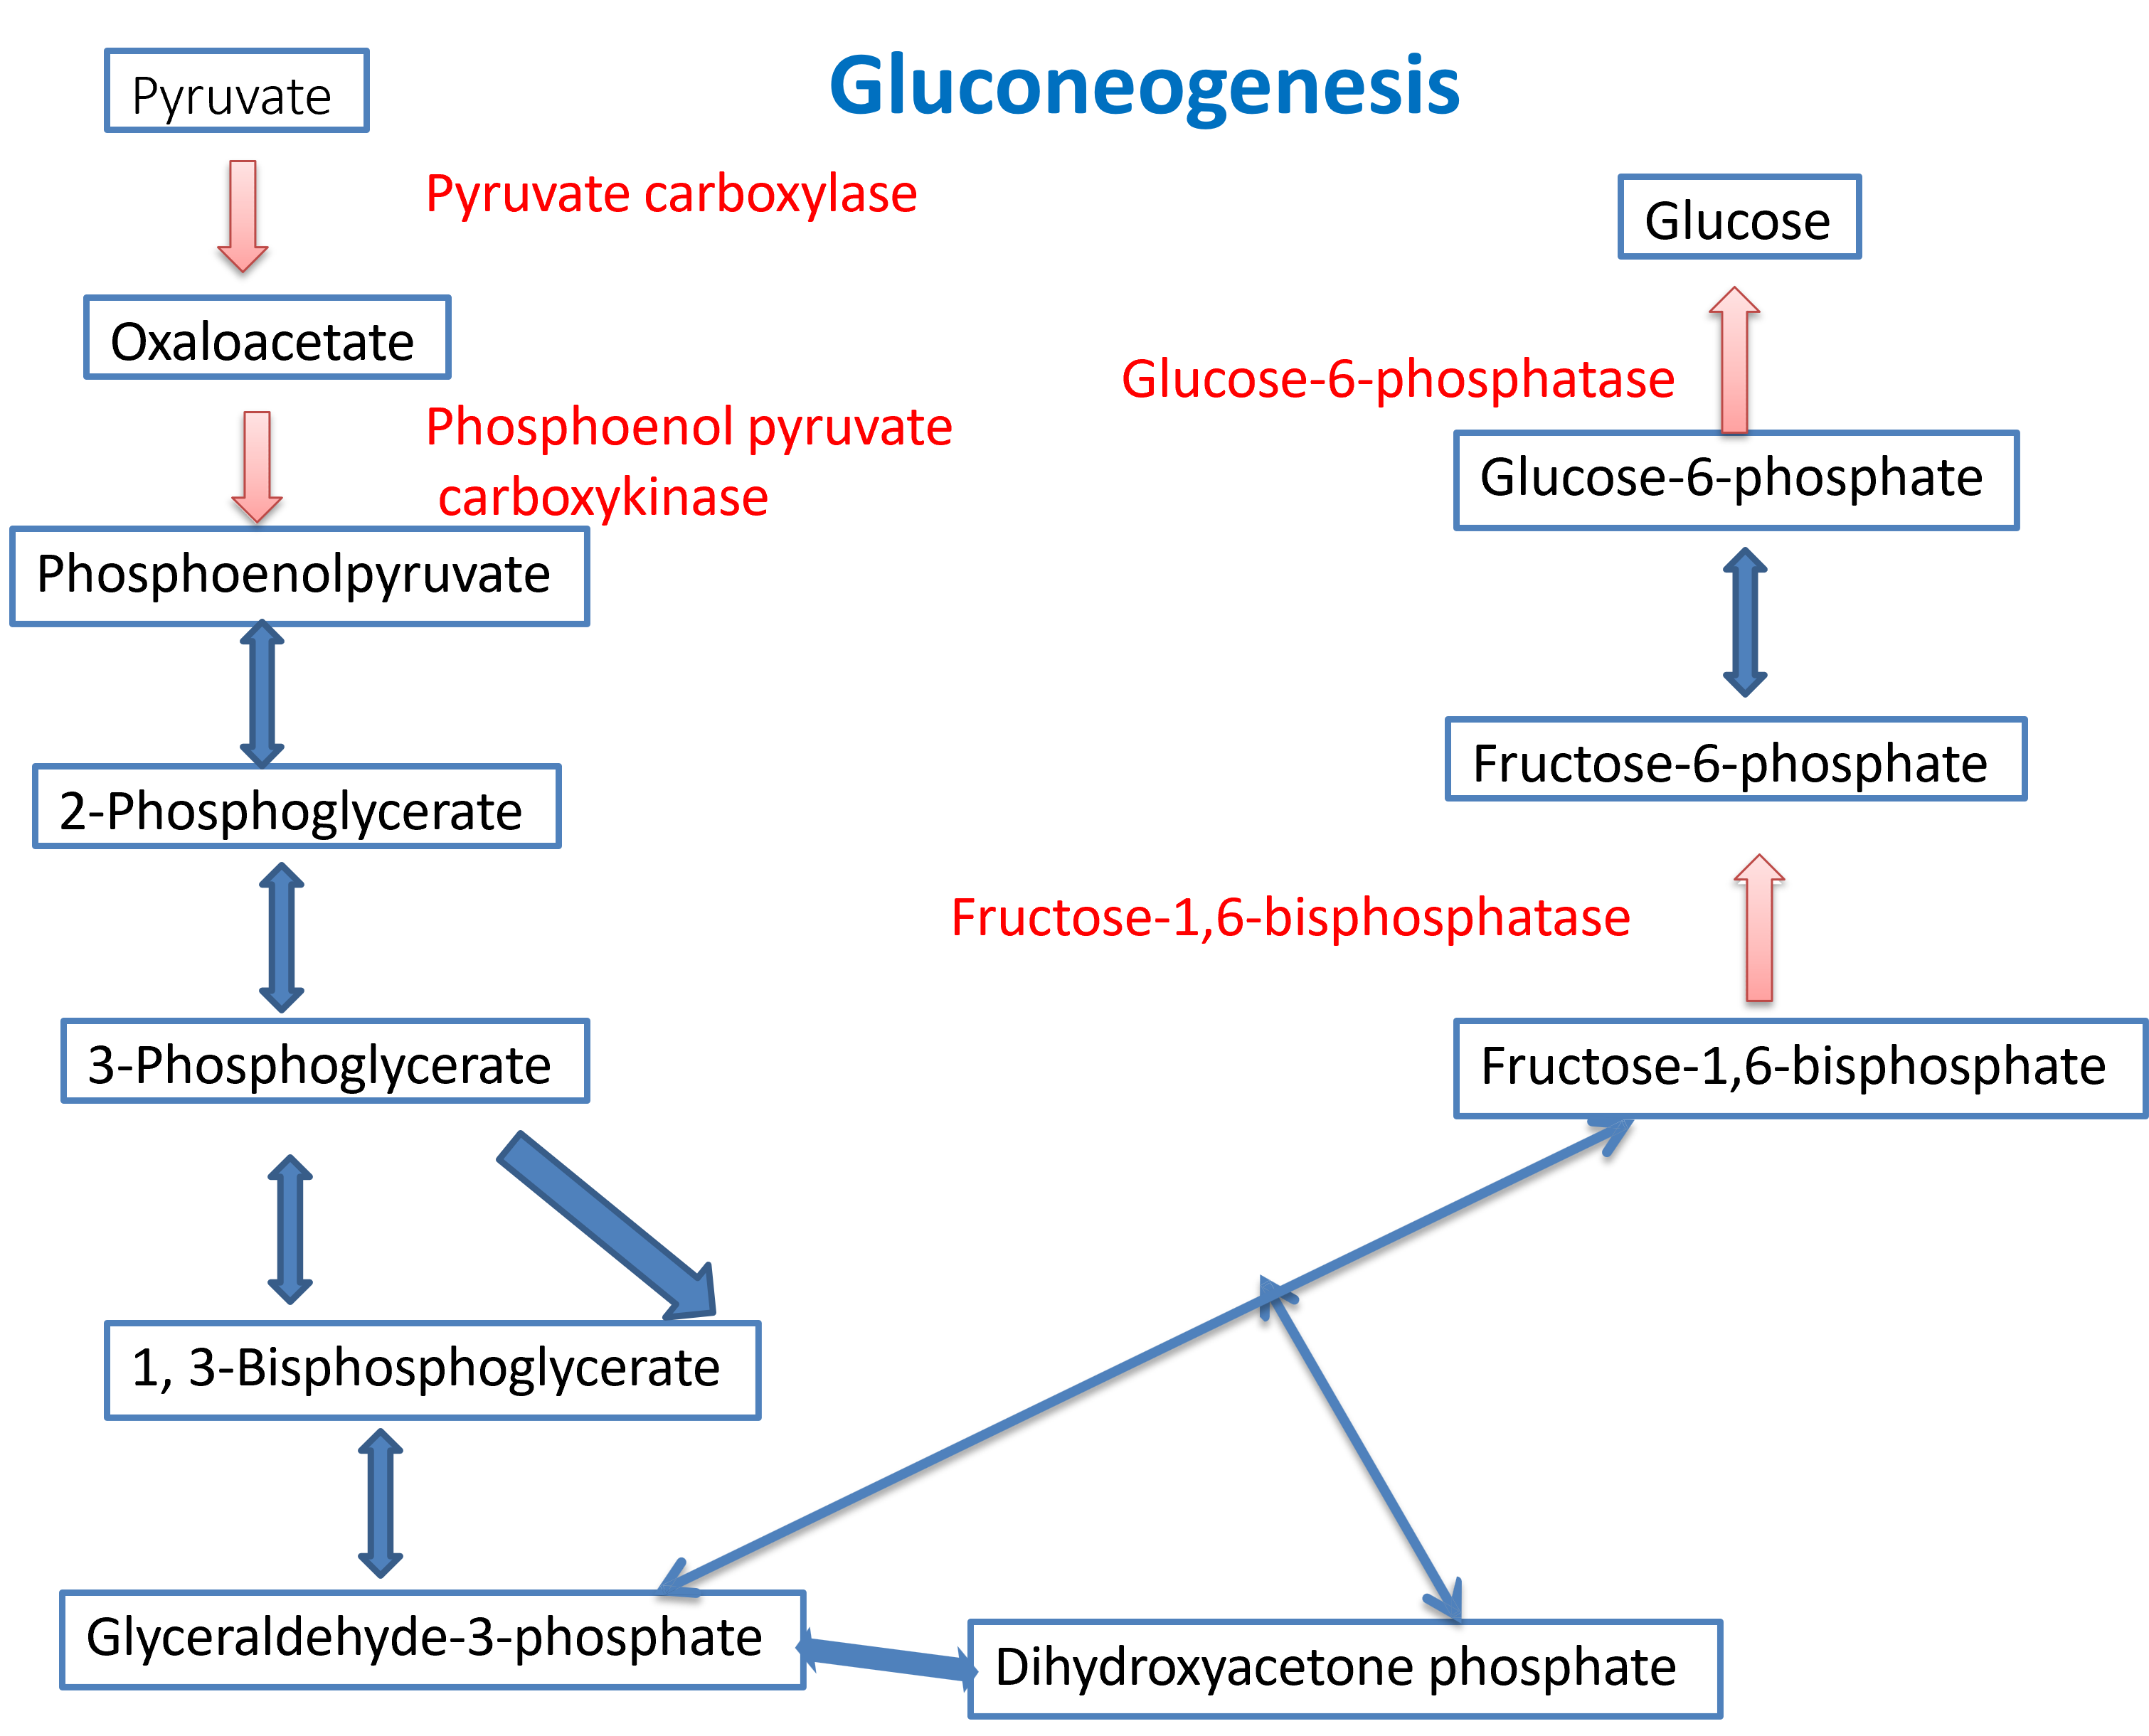
\includegraphics[width=\textwidth,height=3.125in]{Images/gluconeogenesis.png}

\section{Precursors for gluconeogenesis}\label{precursors-for-gluconeogenesis}

Lactate, glucogenic amino acids, glycerol, and propionyl Co-A are the precursors forgluconeogenesis. Lactate is the end product of anaerobic glycolysis in muscle and RBCs. Amino acids are derived from proteins of tissues such as from liver, blood, and muscle. Glycerol is a released from fat during lipolysis. Propionyl Co-A is produced during oxidation of fatty acids with odd number of carbons.

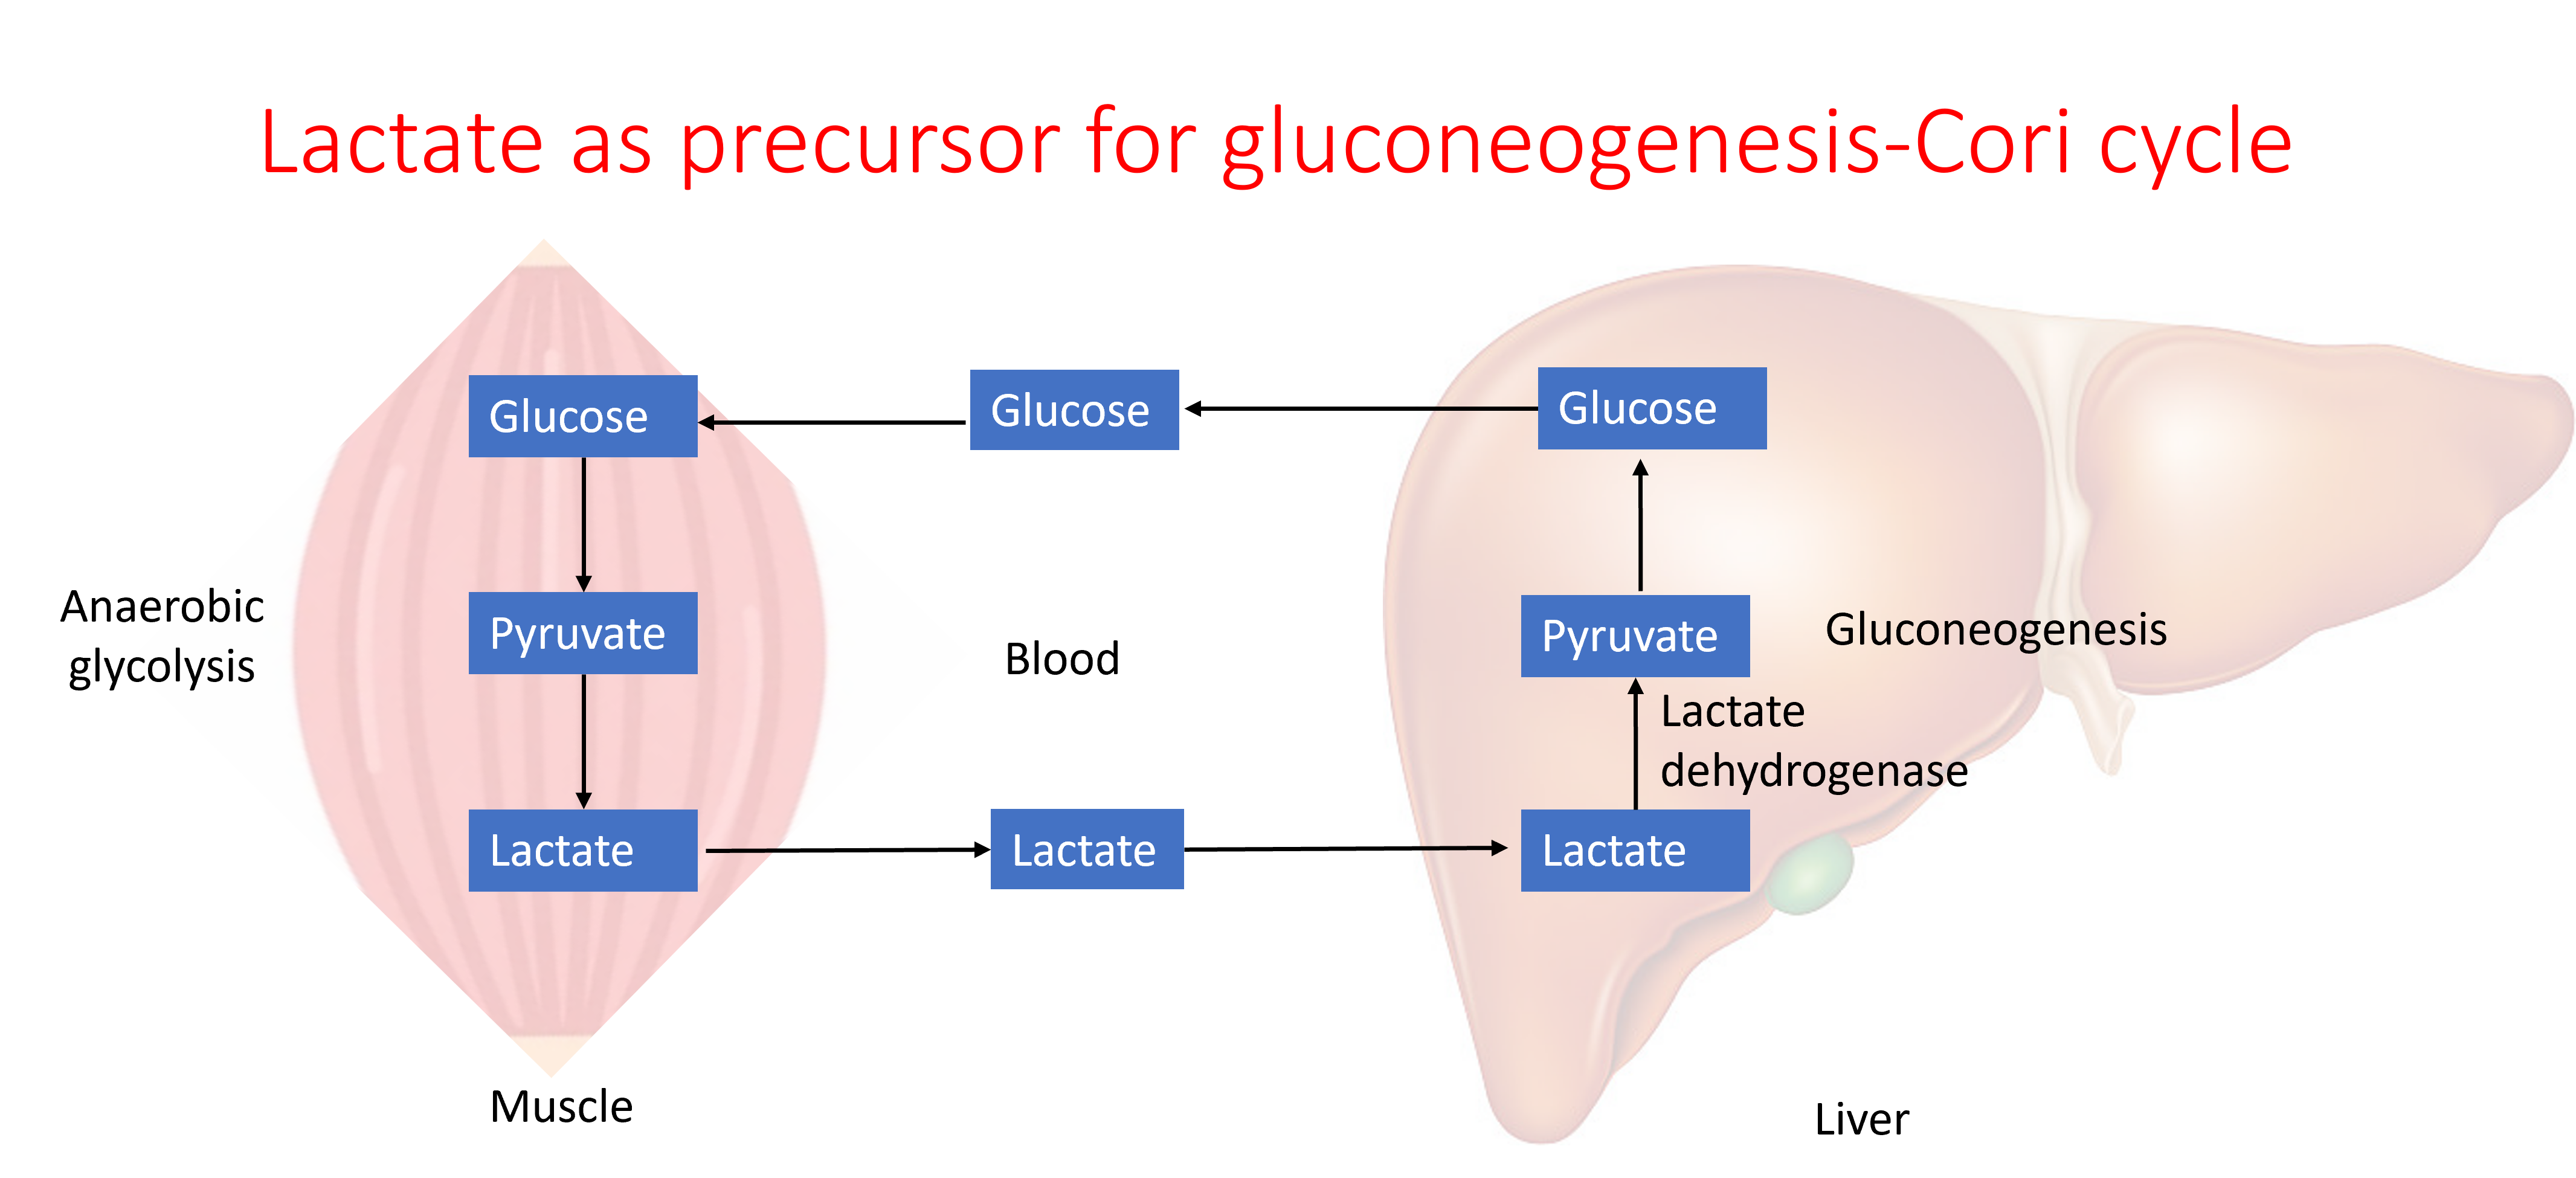
\includegraphics[width=\textwidth,height=3.125in]{Images/cori.png}

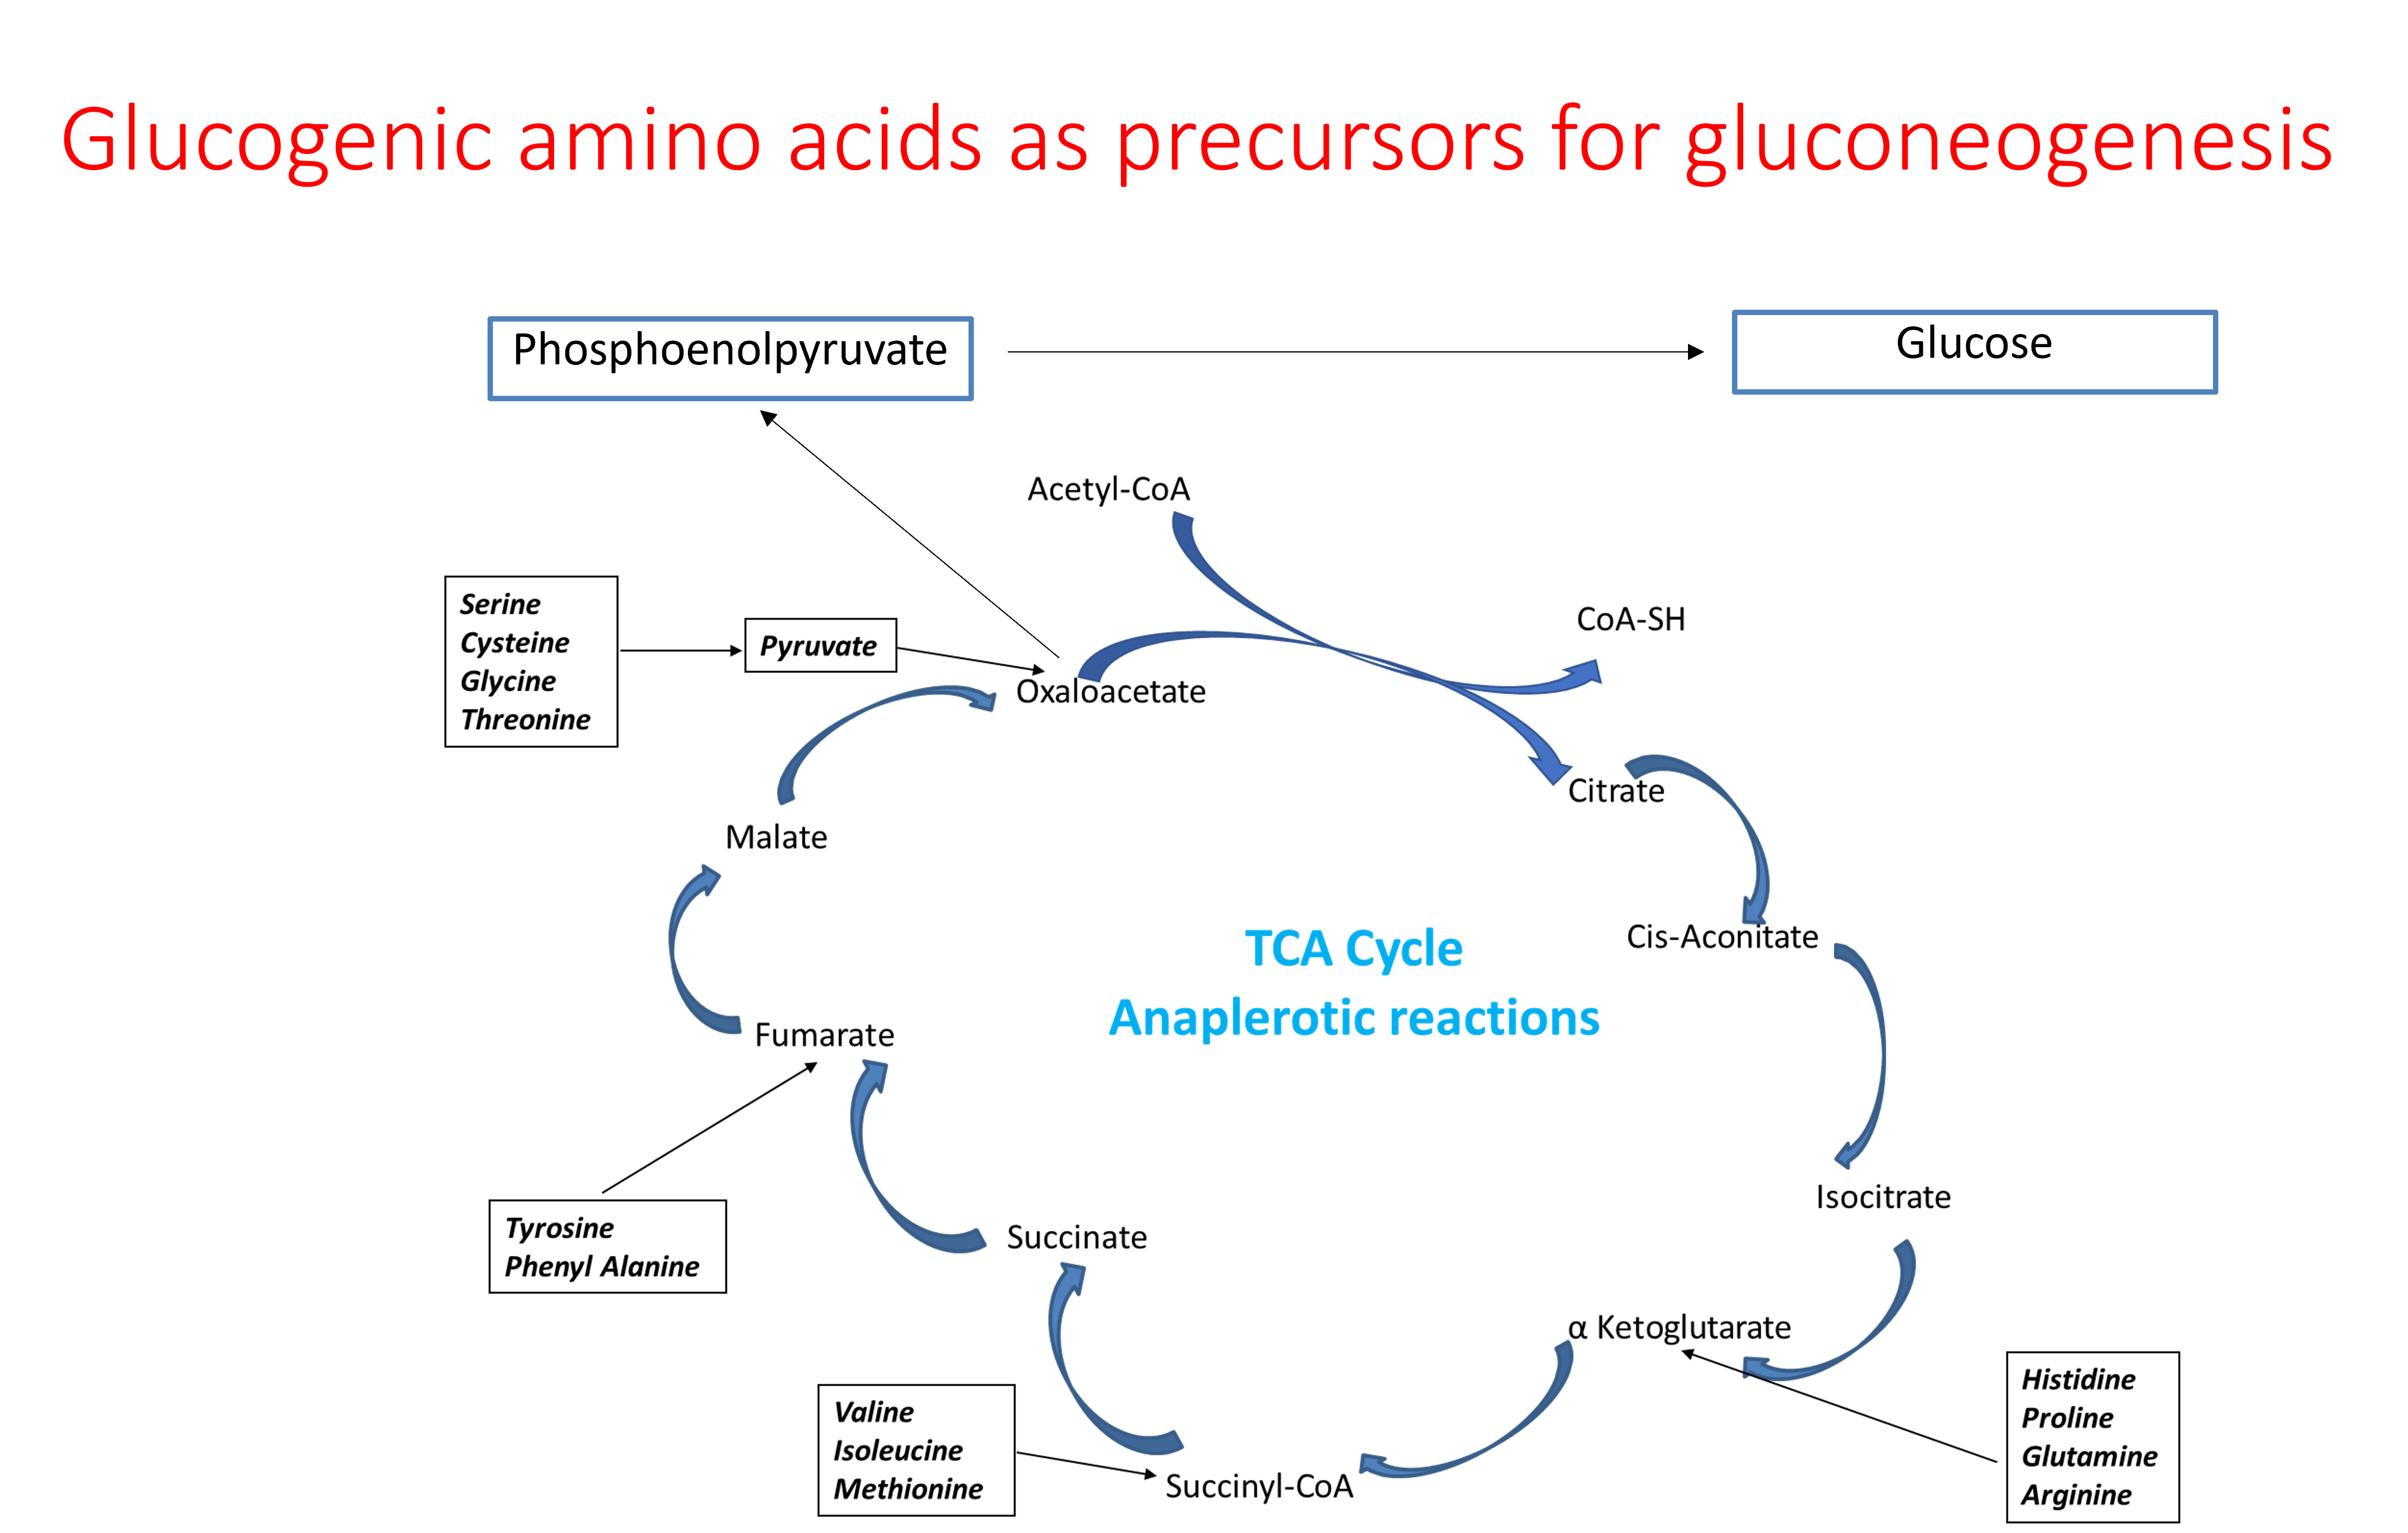
\includegraphics[width=\textwidth,height=4.16667in]{Images/aa.png}

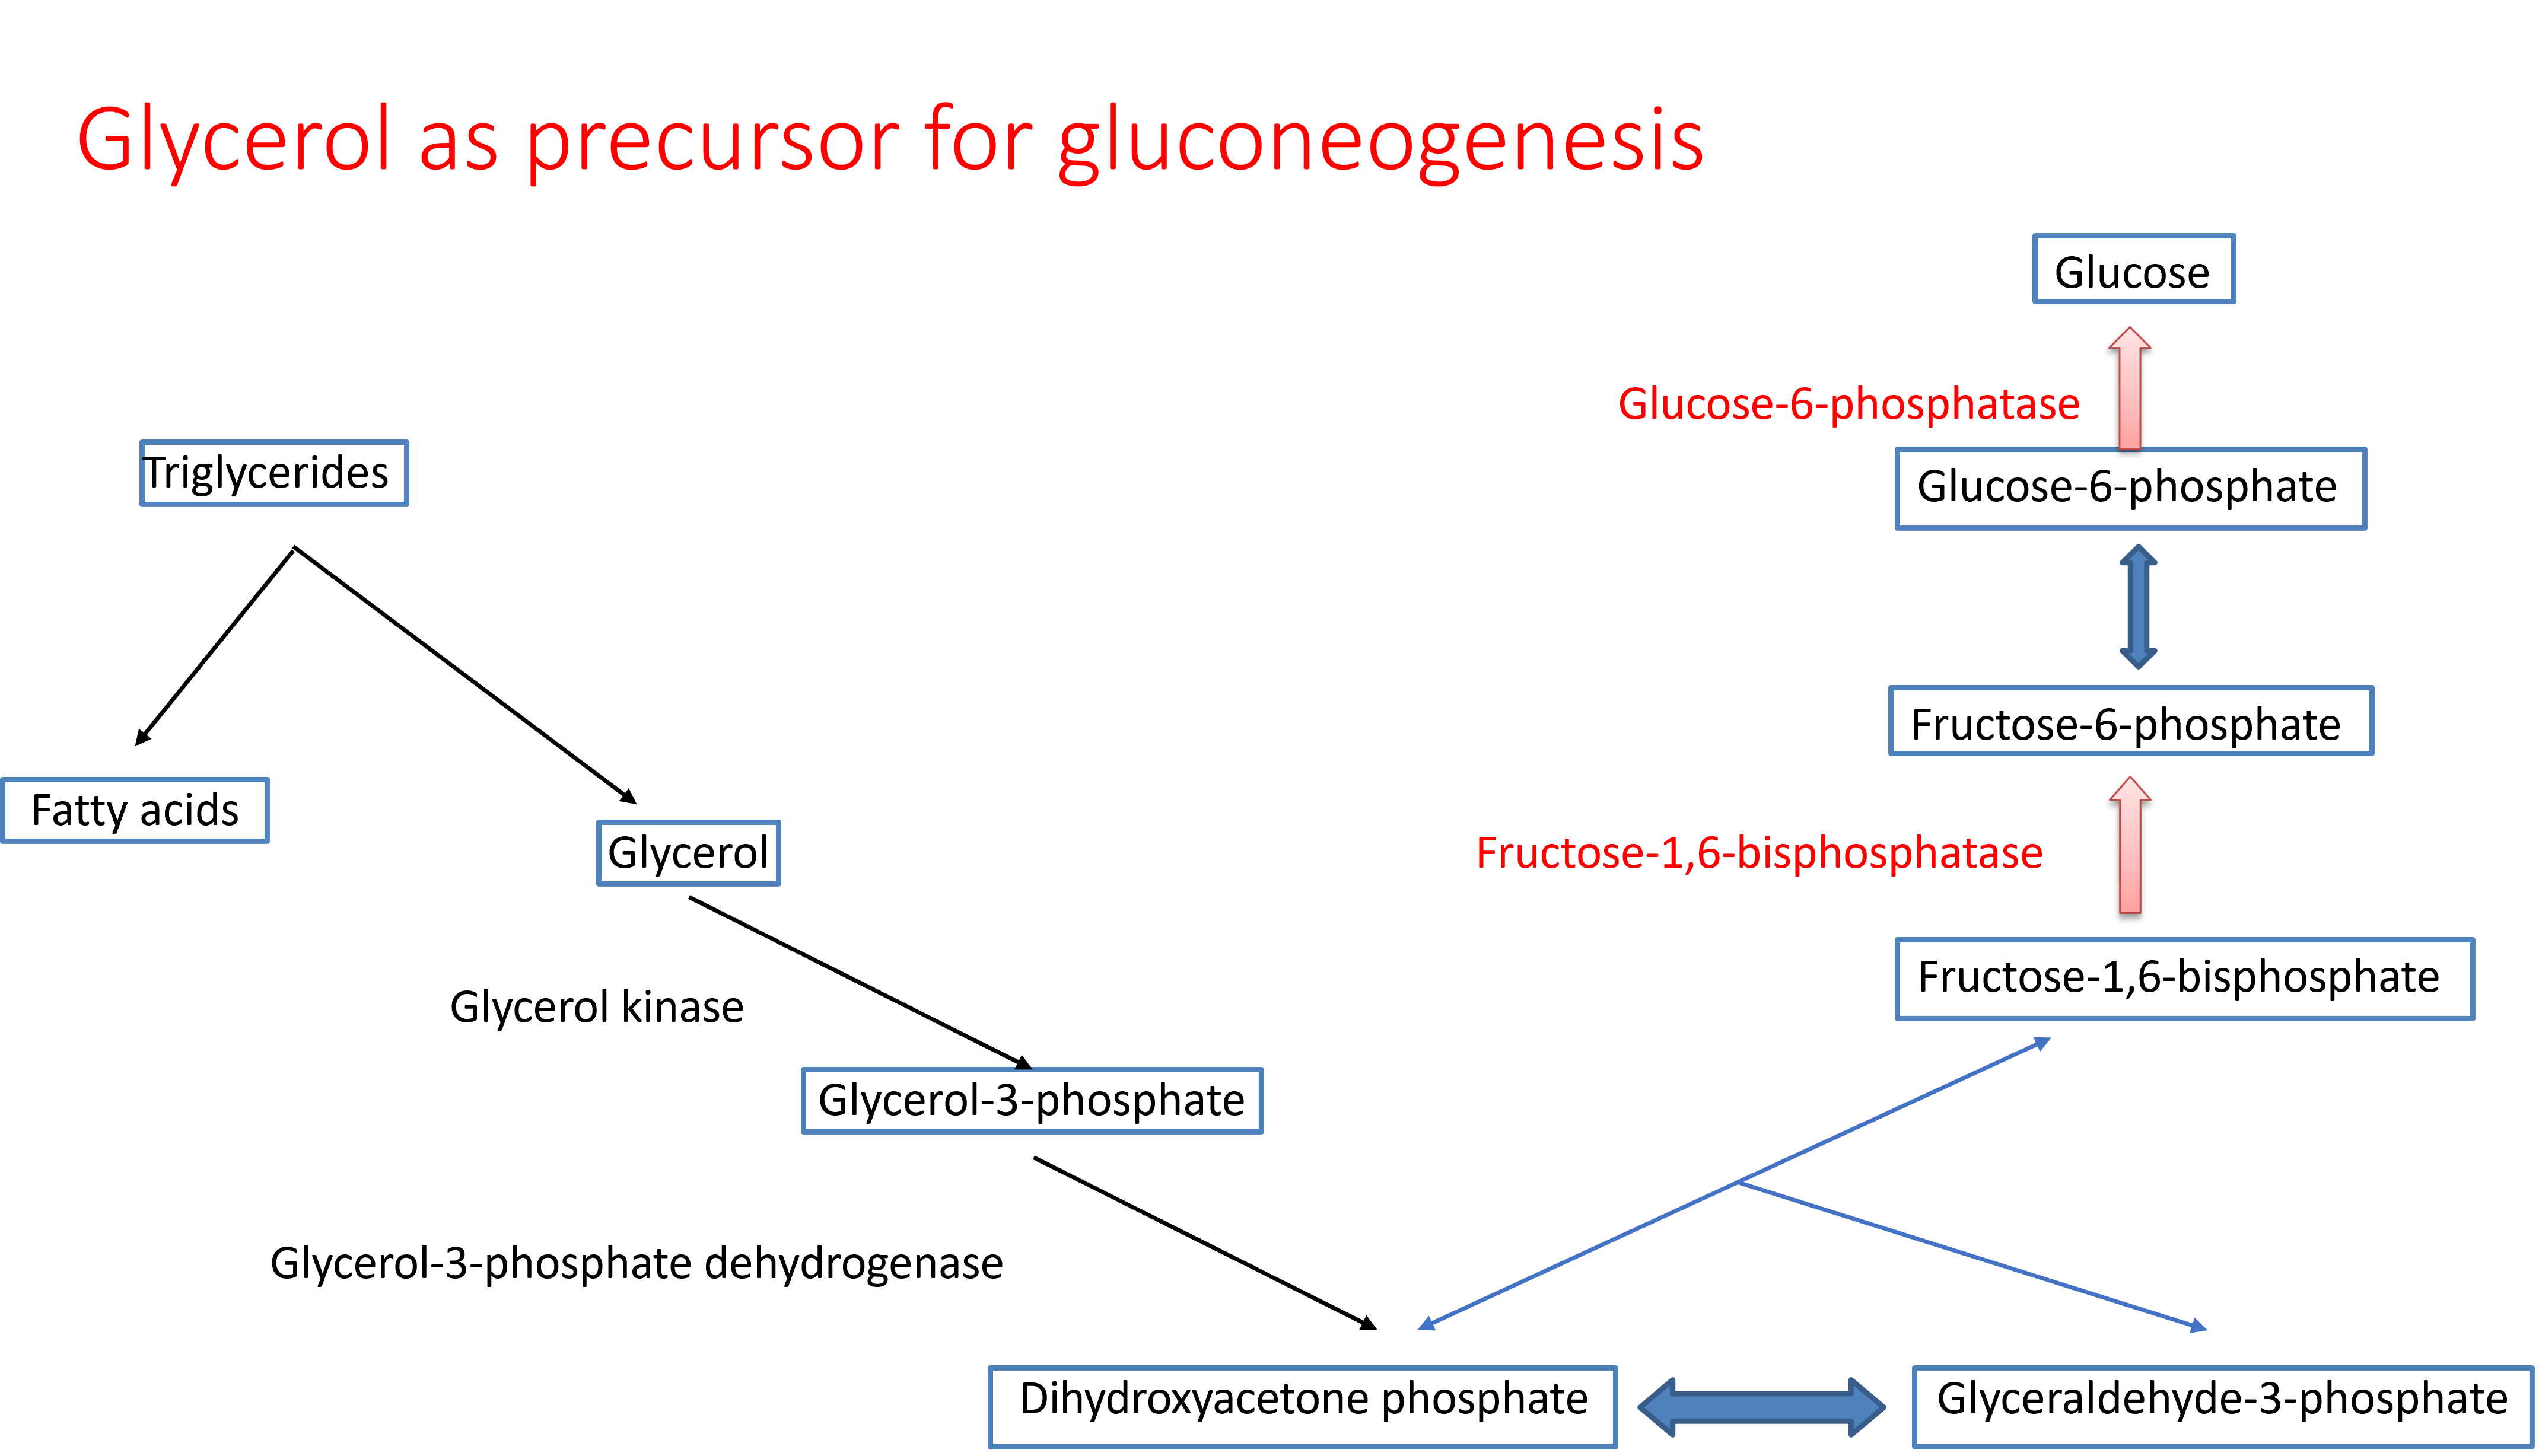
\includegraphics[width=\textwidth,height=3.125in]{Images/glycerol.png}

Gluconeogenesis in liver plays a role in clearing ammmonia produced in the muscle from amino acid catabolism

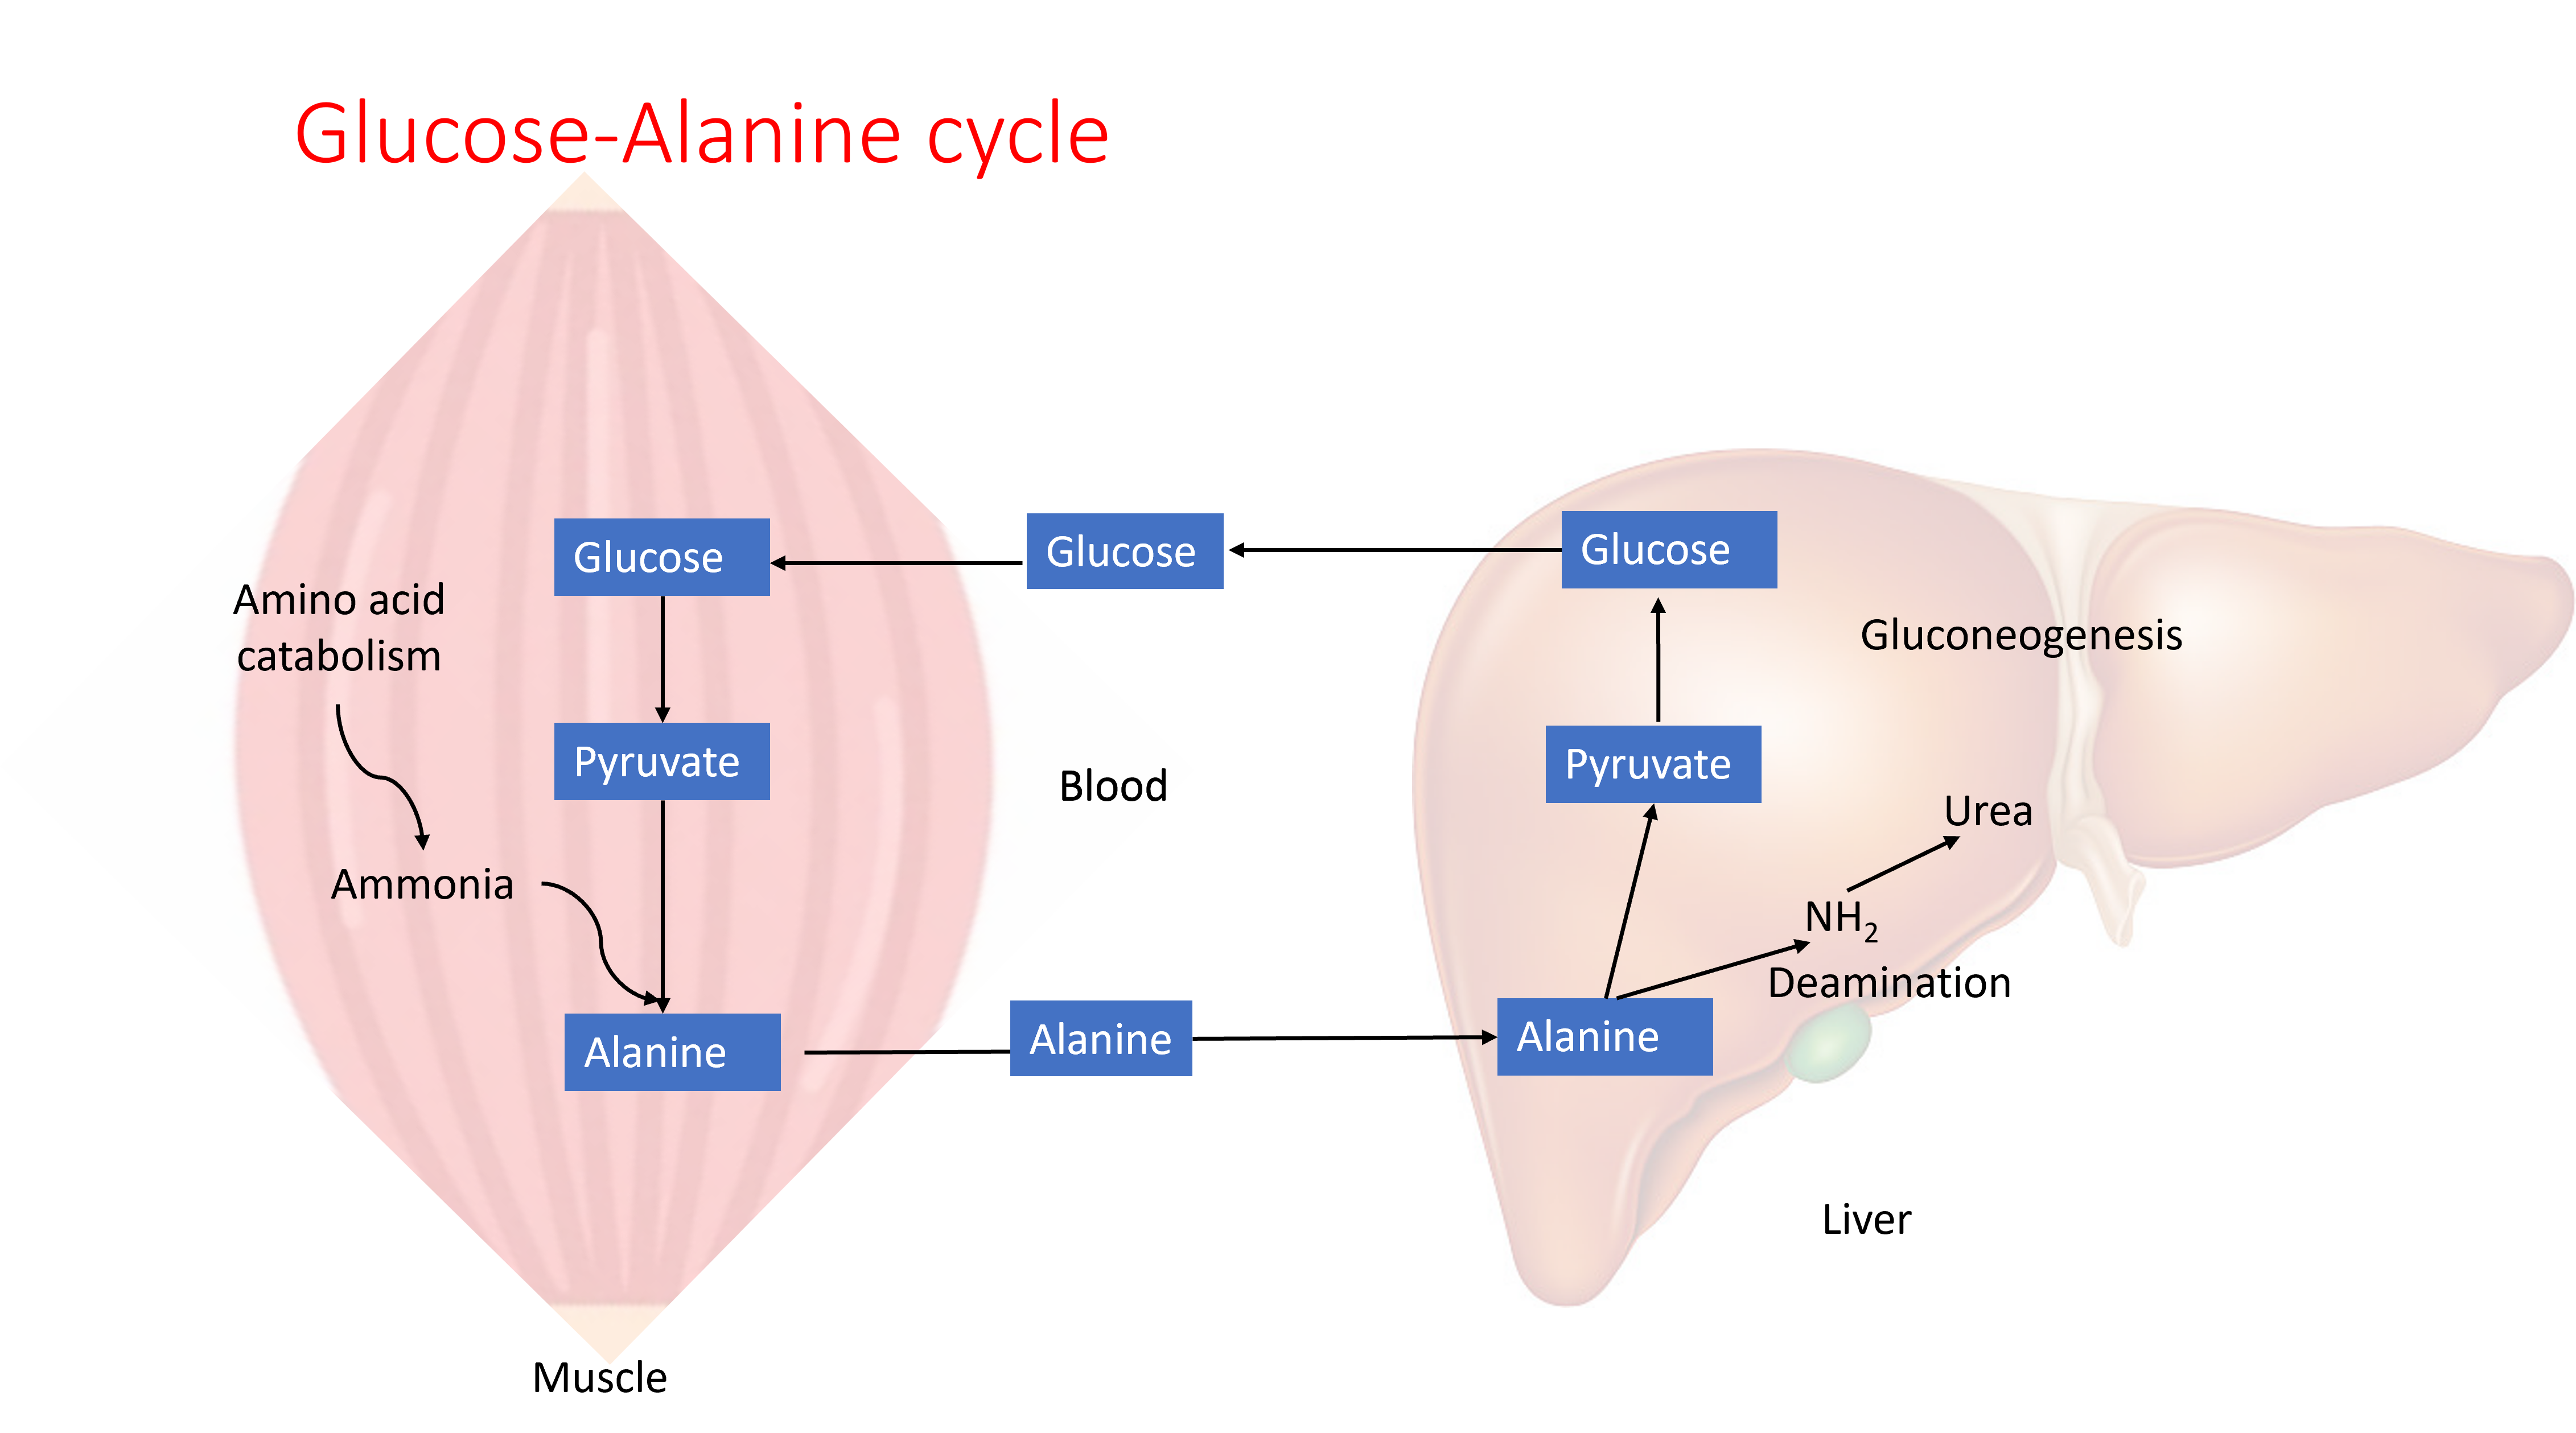
\includegraphics[width=\textwidth,height=3.125in]{Images/alanine.png}

\section{Regulation of glycolysis and gluconeogenesis}\label{regulation-of-glycolysis-and-gluconeogenesis}

Glycolysis and gluconeogenesis are reciprocally regulated. This is achieved by allosteric modification of the enzymes;phosphofructokinase and fructose-1,6-bisphoshatase by Fructose-2,6-bisphosphate. The levels of Fructose-2,6-bisphosphate is regulated by the hormones; insulin and glucagon.

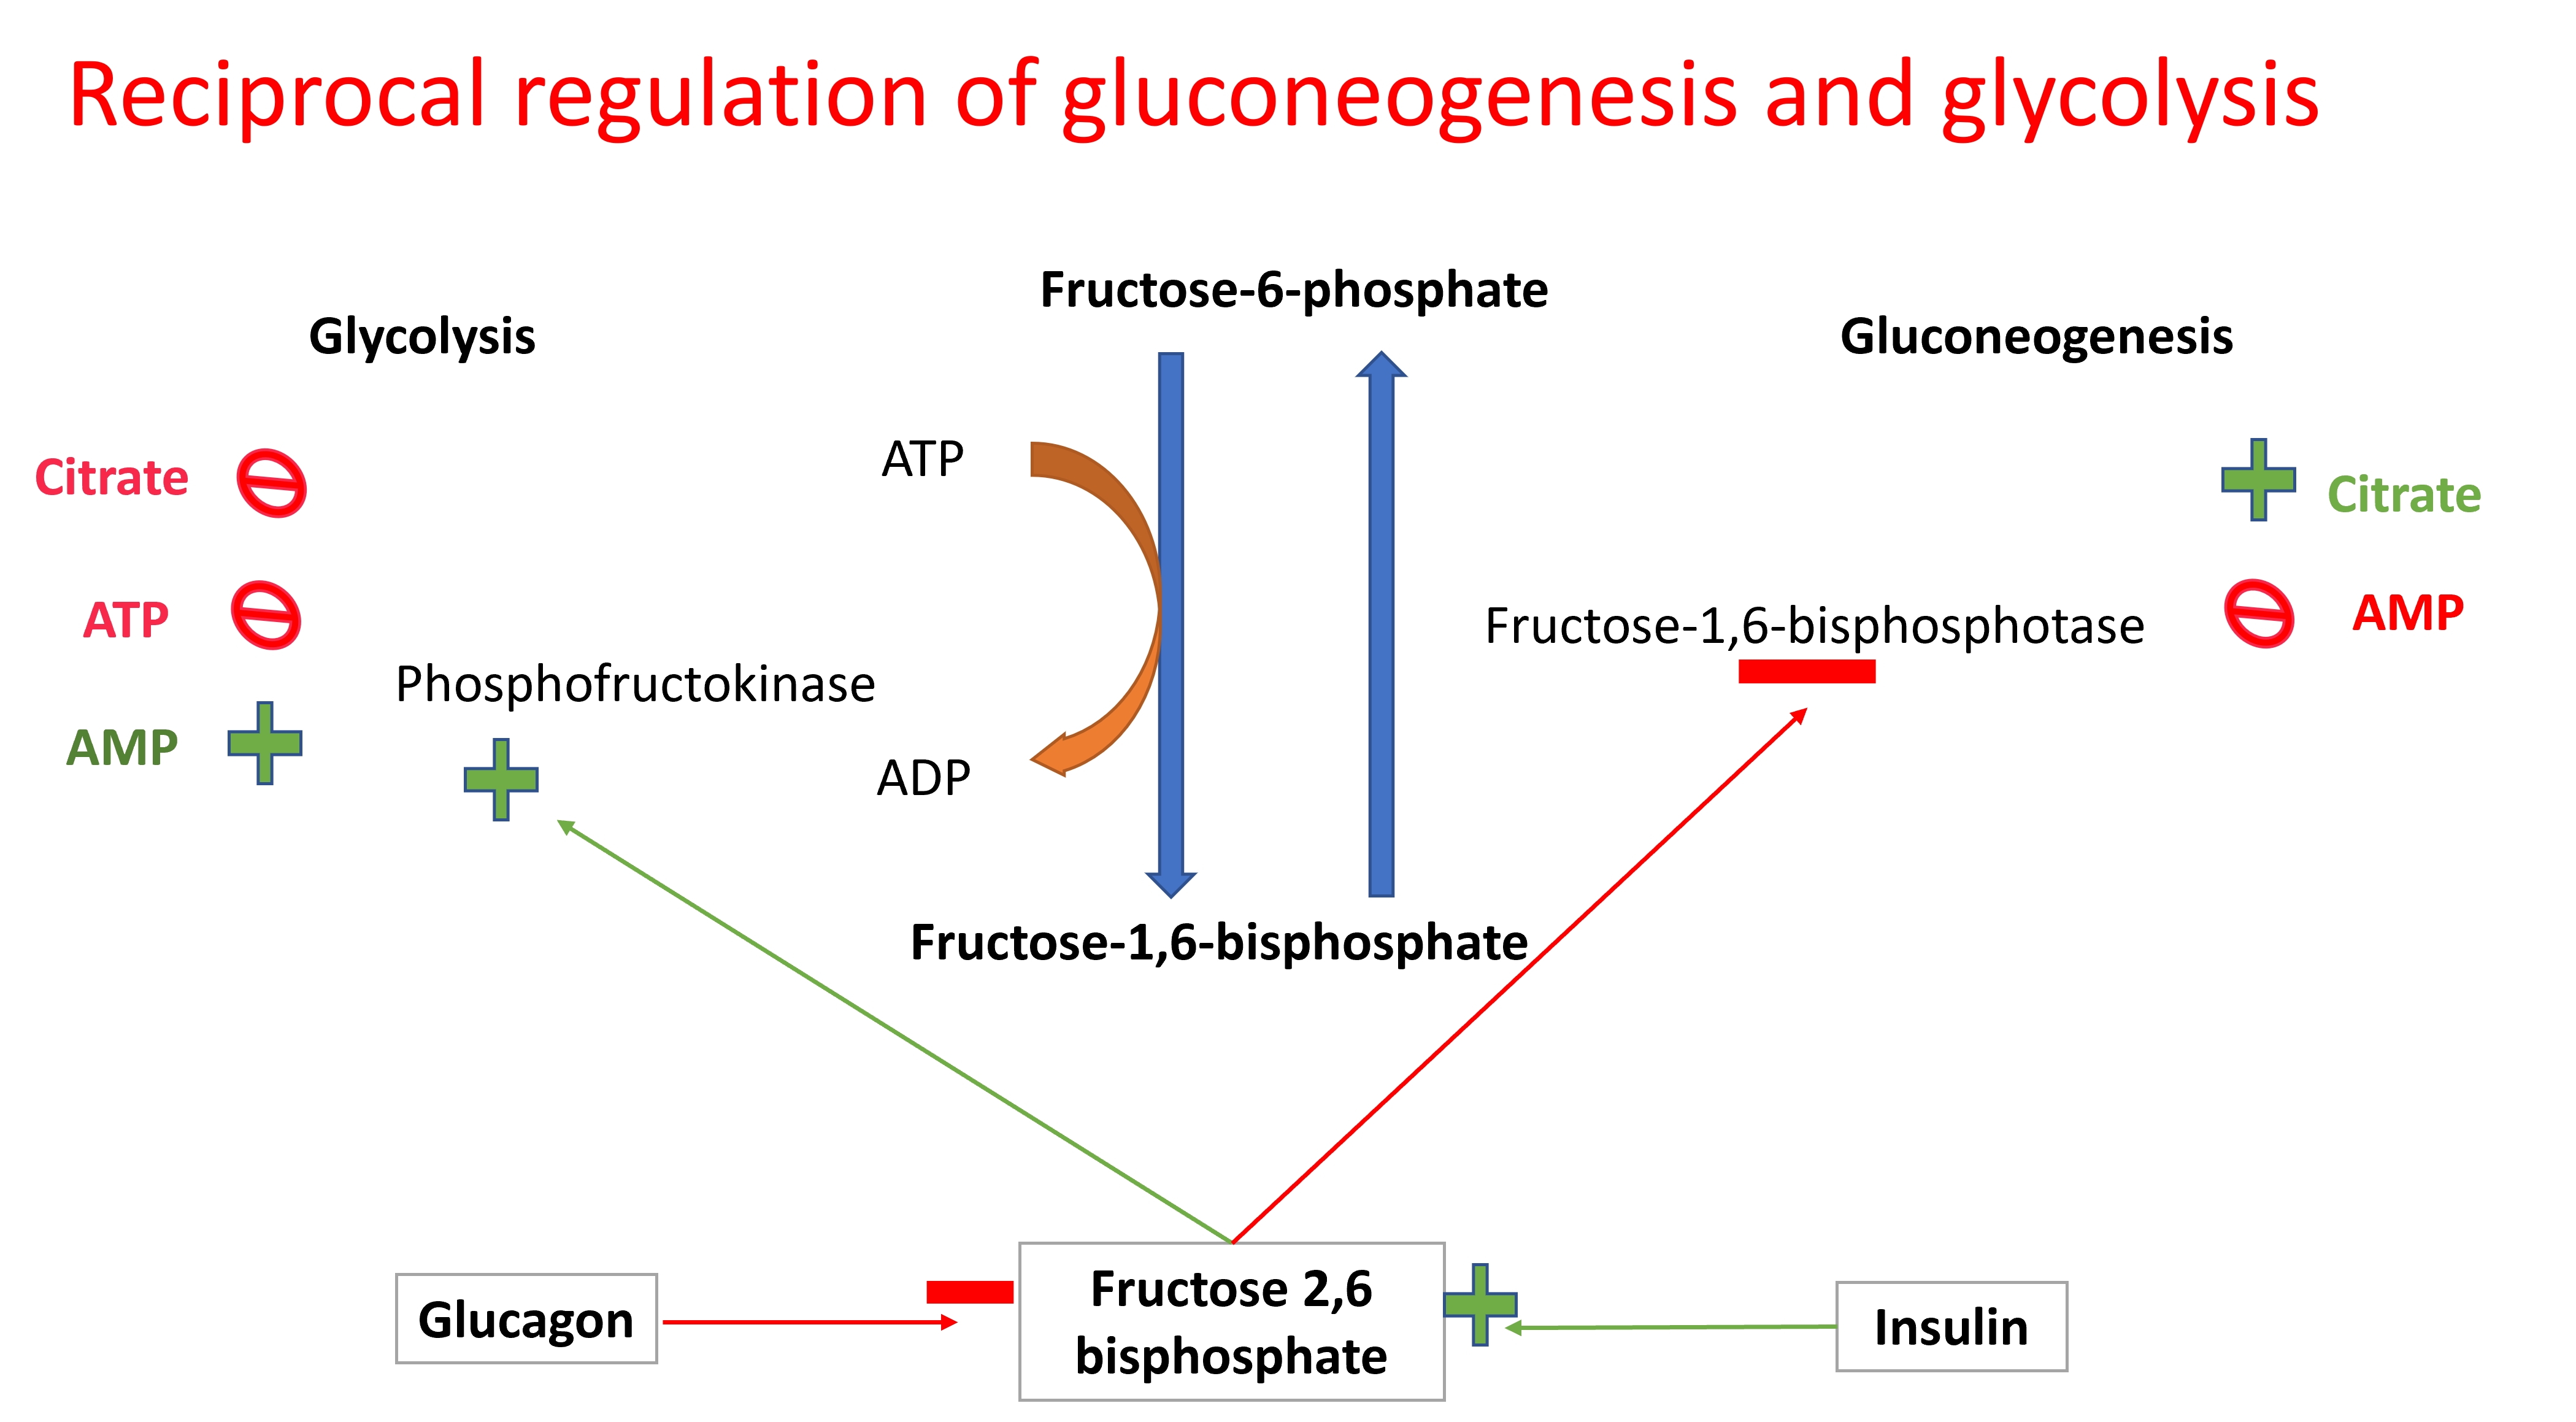
\includegraphics[width=\textwidth,height=3.125in]{Images/reg_gly_gluco.png}
\#\# Practice exercises

\begin{enumerate}
\def\labelenumi{\arabic{enumi}.}
\tightlist
\item
  Which of the following is NOT a substrate for gluconeogenesis?
\end{enumerate}

\begin{itemize}
\tightlist
\item
  \begin{enumerate}
  \def\labelenumi{(\Alph{enumi})}
  \tightlist
  \item
    Acetyl-CoA\\
  \end{enumerate}
\item
  \begin{enumerate}
  \def\labelenumi{(\Alph{enumi})}
  \setcounter{enumi}{1}
  \tightlist
  \item
    Lactate\\
  \end{enumerate}
\item
  \begin{enumerate}
  \def\labelenumi{(\Alph{enumi})}
  \setcounter{enumi}{2}
  \tightlist
  \item
    Glycerol\\
  \end{enumerate}
\item
  \begin{enumerate}
  \def\labelenumi{(\Alph{enumi})}
  \setcounter{enumi}{3}
  \tightlist
  \item
    Alanine
  \end{enumerate}
\end{itemize}

\begin{enumerate}
\def\labelenumi{\arabic{enumi}.}
\setcounter{enumi}{1}
\tightlist
\item
  Match the pathway with its regulated enzyme
\end{enumerate}

\begin{itemize}
\item
  ``Glycogenesis:
\item
  \begin{enumerate}
  \def\labelenumi{(\Alph{enumi})}
  \tightlist
  \item
    Glycogen synthase\\
  \end{enumerate}
\item
  \begin{enumerate}
  \def\labelenumi{(\Alph{enumi})}
  \setcounter{enumi}{1}
  \tightlist
  \item
    Glycogen phosphorylase\\
  \end{enumerate}
\item
  \begin{enumerate}
  \def\labelenumi{(\Alph{enumi})}
  \setcounter{enumi}{2}
  \tightlist
  \item
    Fructose 1,6-Bisphosphatase\\
  \end{enumerate}
\item
  \begin{enumerate}
  \def\labelenumi{(\Alph{enumi})}
  \setcounter{enumi}{3}
  \tightlist
  \item
    Phosphofructokinase-1
  \end{enumerate}
\end{itemize}

''

\begin{itemize}
\item
  ``Glycogenolysis:
\item
  \begin{enumerate}
  \def\labelenumi{(\Alph{enumi})}
  \tightlist
  \item
    Glycogen synthase\\
  \end{enumerate}
\item
  \begin{enumerate}
  \def\labelenumi{(\Alph{enumi})}
  \setcounter{enumi}{1}
  \tightlist
  \item
    Glycogen phosphorylase\\
  \end{enumerate}
\item
  \begin{enumerate}
  \def\labelenumi{(\Alph{enumi})}
  \setcounter{enumi}{2}
  \tightlist
  \item
    Fructose 1,6-Bisphosphatase\\
  \end{enumerate}
\item
  \begin{enumerate}
  \def\labelenumi{(\Alph{enumi})}
  \setcounter{enumi}{3}
  \tightlist
  \item
    Phosphofructokinase-1
  \end{enumerate}
\end{itemize}

''

\begin{itemize}
\item
  ``Gluconeogenesis:
\item
  \begin{enumerate}
  \def\labelenumi{(\Alph{enumi})}
  \tightlist
  \item
    Glycogen synthase\\
  \end{enumerate}
\item
  \begin{enumerate}
  \def\labelenumi{(\Alph{enumi})}
  \setcounter{enumi}{1}
  \tightlist
  \item
    Glycogen phosphorylase\\
  \end{enumerate}
\item
  \begin{enumerate}
  \def\labelenumi{(\Alph{enumi})}
  \setcounter{enumi}{2}
  \tightlist
  \item
    Fructose 1,6-Bisphosphatase\\
  \end{enumerate}
\item
  \begin{enumerate}
  \def\labelenumi{(\Alph{enumi})}
  \setcounter{enumi}{3}
  \tightlist
  \item
    Phosphofructokinase-1
  \end{enumerate}
\end{itemize}

''

\chapter{Regulation of blood glucose}\label{regulation-of-blood-glucose}

Glucose is a major source of fuel for all cells. Brain and RBCs are completely dependent on glucose for producing energy. Decrease in blood glucose level, called hypoglycemia can lead to impaired function of the brain since glucose is the only source of energy for the brain. If severe, hypoglycemia can cause coma and death. On the other hand, chronic increase in blood glucose level can damage multiple tissues. This is seen in diabetes mellitus.Thus blood glucose level has to be maintained within a narrow range of 70 to 99 mg/dL./

Blood glucose level is maintained within this narrow range by processes that utilize glucose during feeding and processes that mobilize and synthesize glucose fasting./

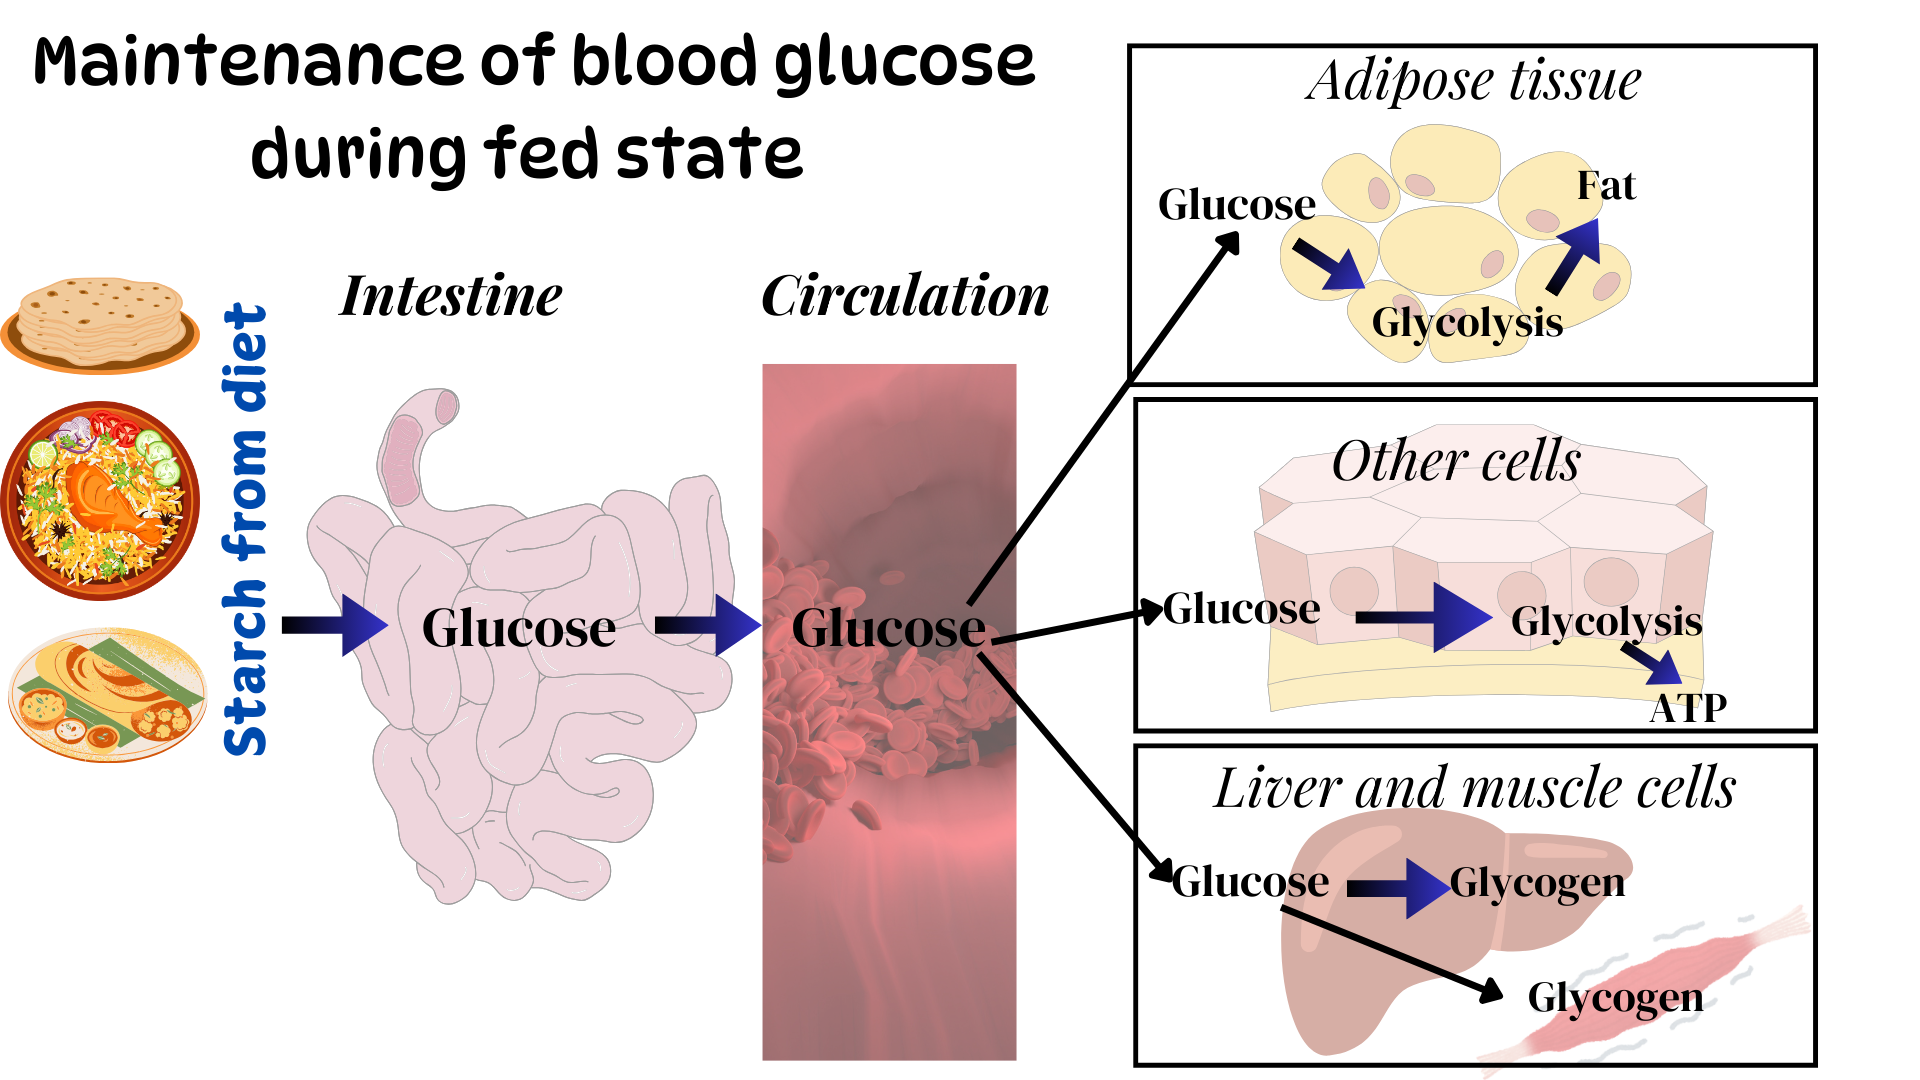
\includegraphics[width=\textwidth,height=4.16667in]{Images/feeding.png}
\footnote{Made by Dr.Monica Peter}

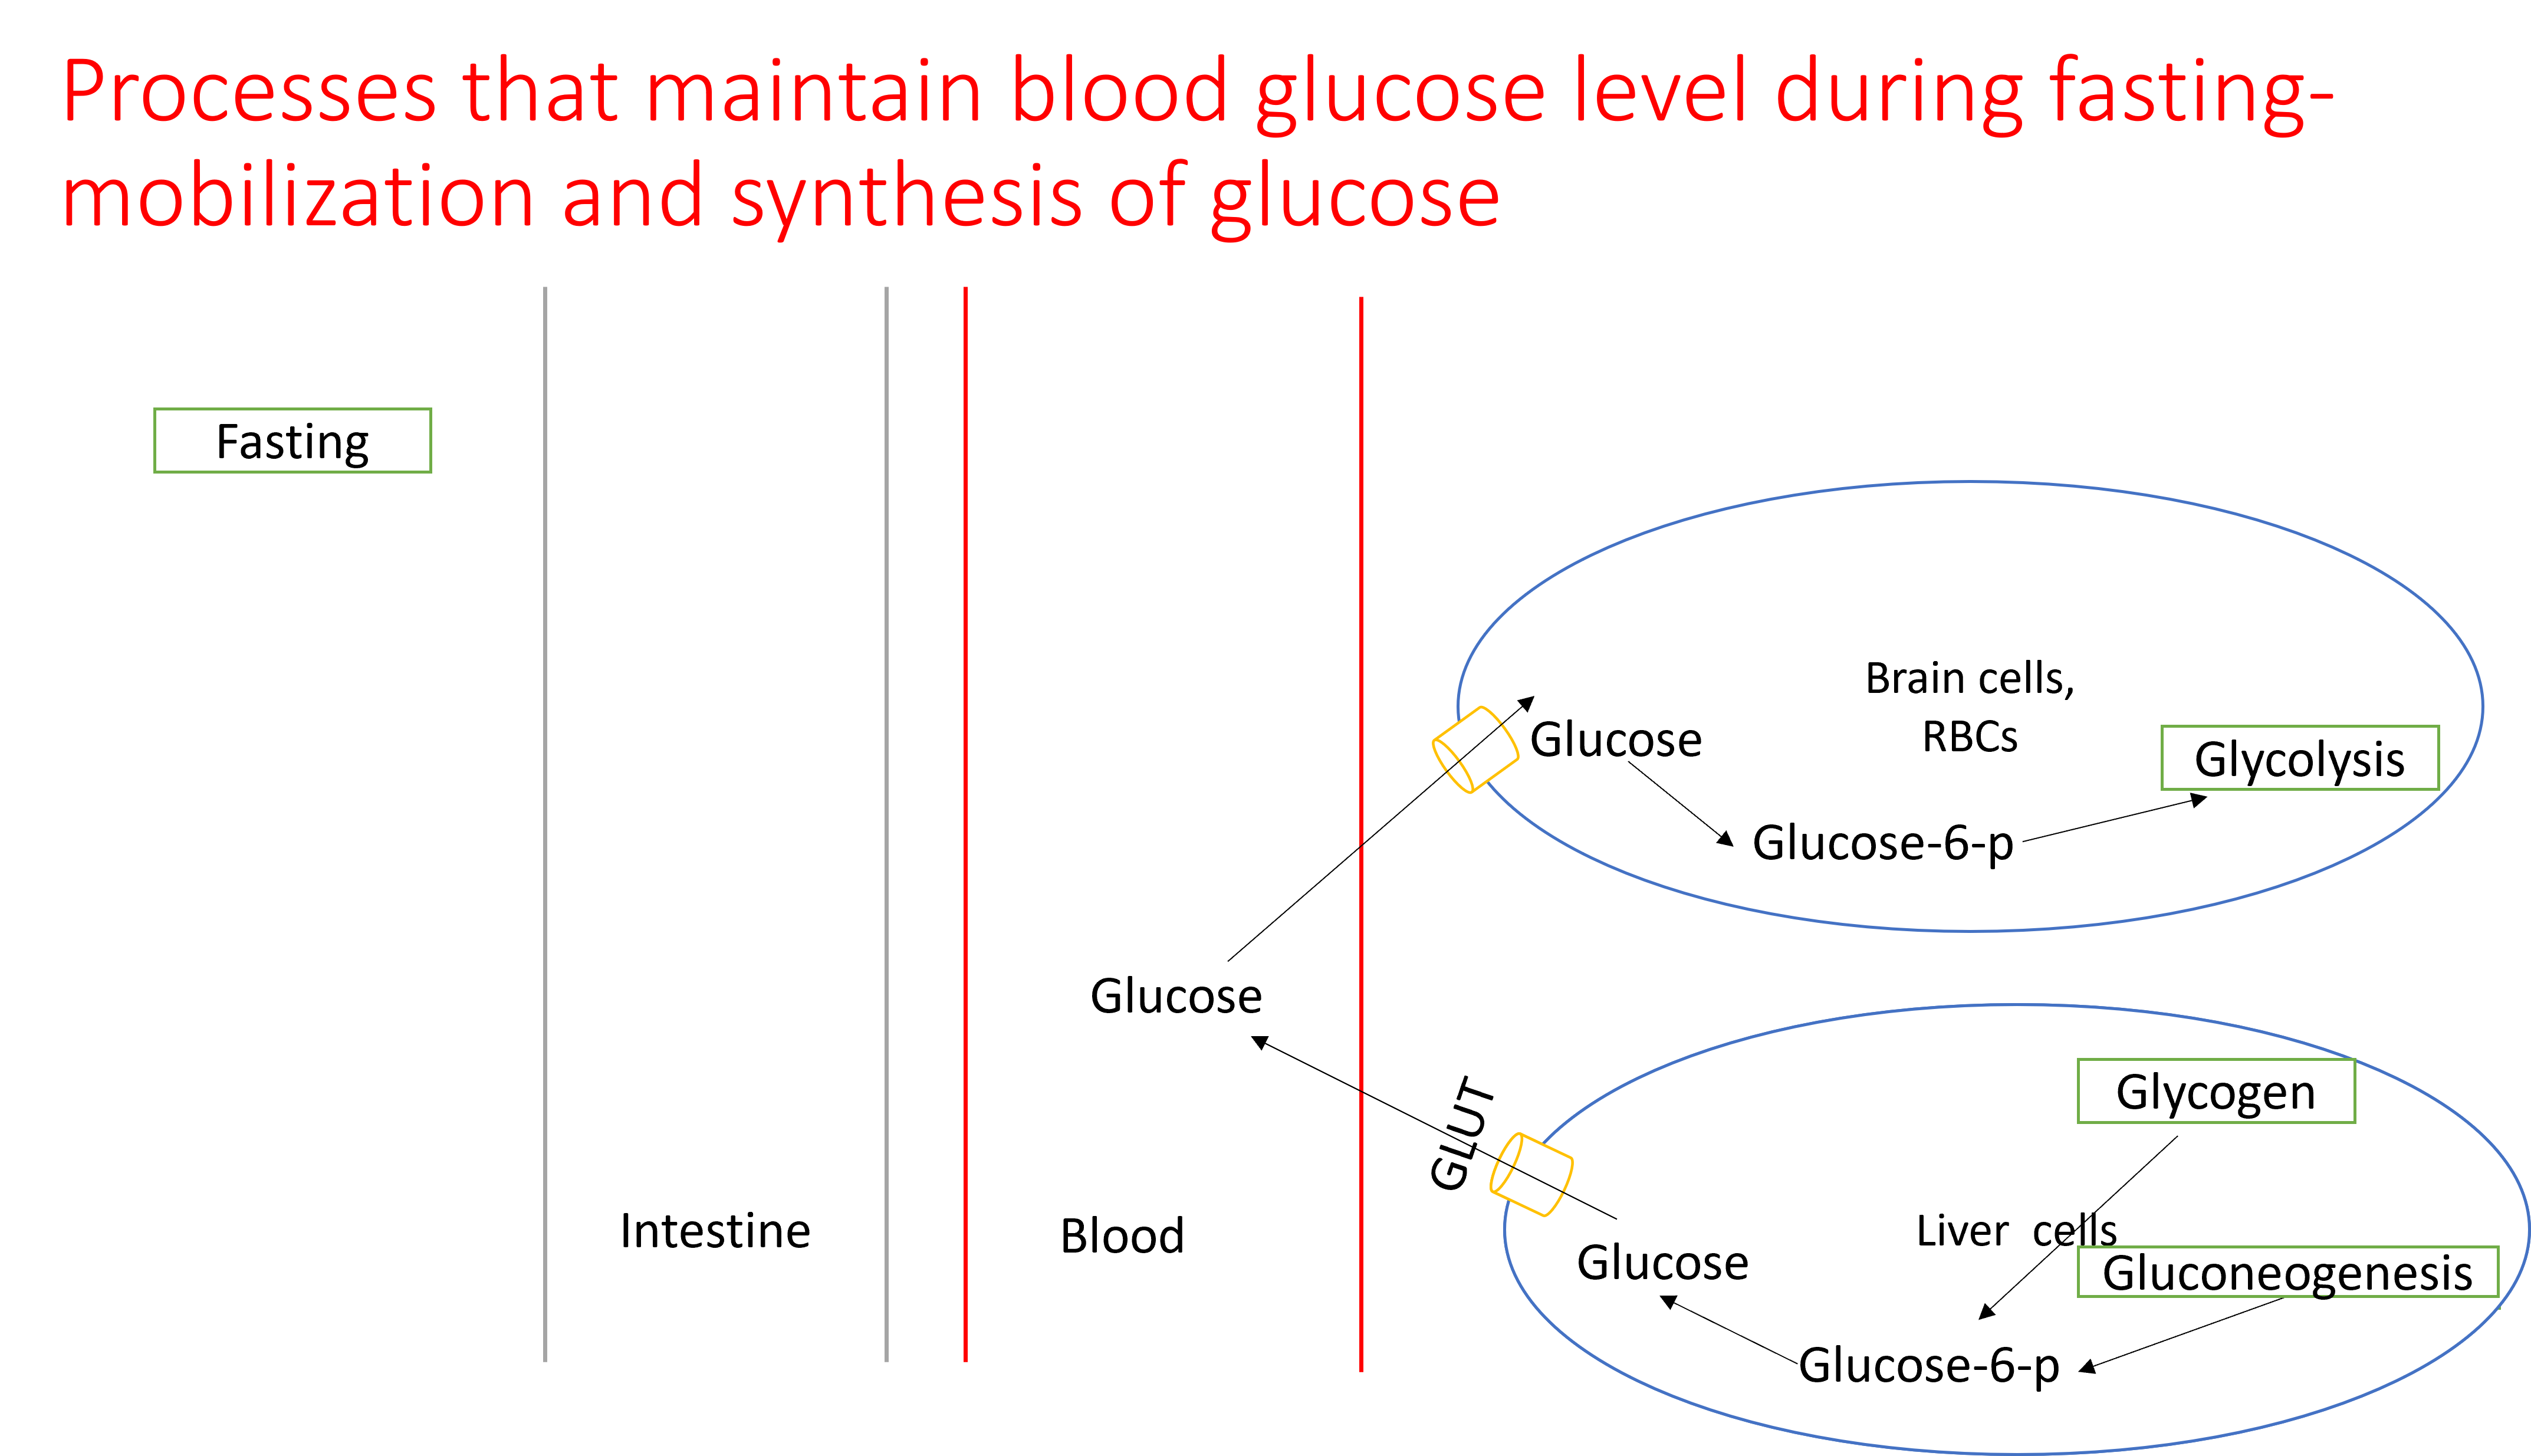
\includegraphics[width=\textwidth,height=4.16667in]{Images/fasting.png}

These processes are regulated by the peptide hormones insulin and glucagon./

\section{Insulin}\label{insulin}

Insulin is a peptide hormone secreted by the beta-cells of the pancreatic islets in response to increase in blood glucose level during feeding.

\subsection{Mechanism of glucose stimulated insulin secretion}\label{mechanism-of-glucose-stimulated-insulin-secretion}

\subsection{Actions of insulin}\label{actions-of-insulin}

Insulin stimulates glucose utilization and inhibits glucose production resulting in decrease in blood glucose level. Insulin increases uptake of glucose into adipose tissue and muscle through activation of \hyperref[glucose-transporters]{GLUT4 transporters}.Insulin \hyperref[regulation-of-glycolysis-and-gluconeogenesis]{stimulates glycolysis and inhibits gluconeogenesis} in liver by increasing the levels of Fructose-2,6 bisphosphate. \hyperref[hormonal-regulation-of-glycogen-metabolism]{Insulin inactivates glycogen phosphorylase and activates glycogen sythase through covalent modifications resulting in activation of glyocgenesis and inhibition of glycogenolysis in liver and muscle}. Insulin also promotes the conversion of glucose to fat in adipose tissue.

\section{Glucagon}\label{glucagon}

Glucagon is a peptide hormone secreted from the alpha-cells of the pancreatic islets in response to decrease in blood glucose level during fasting. Glucagon stimulates glucose mobilization and promotes glucose production resulting in increase in blood glucose level.

\subsection{Actions of glucagon}\label{actions-of-glucagon}

Glucagon \hyperref[regulation-of-glycolysis-and-gluconeogenesis]{stimulates gluconeogenesis and inhibits glycolysis} in liver by decreasing the levels of Fructose-2,6 bisphosphate. \hyperref[hormonal-regulation-of-glycogen-metabolism]{Glucagon inactivates glycogen synthase and activates glycogen phosphorylase through covalent modifications resulting in activation of glycogenolysis and inhibition of glyocgenesis in liver and muscle}./

Epinephrine, cortisol, thyroxine, and growth hormone are other hormones that can blood glucose levels.

\section{Practice exercises}\label{practice-exercises-4}

\begin{enumerate}
\def\labelenumi{\arabic{enumi}.}
\tightlist
\item
  Which of the following is an effect of insulin?
\end{enumerate}

\begin{itemize}
\tightlist
\item
  \begin{enumerate}
  \def\labelenumi{(\Alph{enumi})}
  \tightlist
  \item
    Increased glycogenolysis in liver\\
  \end{enumerate}
\item
  \begin{enumerate}
  \def\labelenumi{(\Alph{enumi})}
  \setcounter{enumi}{1}
  \tightlist
  \item
    Increased gluconeogenesis in liver\\
  \end{enumerate}
\item
  \begin{enumerate}
  \def\labelenumi{(\Alph{enumi})}
  \setcounter{enumi}{2}
  \tightlist
  \item
    Increased glucose uptake in adipose tissue and muscle\\
  \end{enumerate}
\item
  \begin{enumerate}
  \def\labelenumi{(\Alph{enumi})}
  \setcounter{enumi}{3}
  \tightlist
  \item
    Decreased glycolysis in liver
  \end{enumerate}
\end{itemize}

\begin{enumerate}
\def\labelenumi{\arabic{enumi}.}
\setcounter{enumi}{1}
\tightlist
\item
  Which of the following is an effect of glucagon?
\end{enumerate}

\begin{itemize}
\tightlist
\item
  \begin{enumerate}
  \def\labelenumi{(\Alph{enumi})}
  \tightlist
  \item
    Decreased gluconeogenesis in liver\\
  \end{enumerate}
\item
  \begin{enumerate}
  \def\labelenumi{(\Alph{enumi})}
  \setcounter{enumi}{1}
  \tightlist
  \item
    Increased glycogenolysis in liver\\
  \end{enumerate}
\item
  \begin{enumerate}
  \def\labelenumi{(\Alph{enumi})}
  \setcounter{enumi}{2}
  \tightlist
  \item
    Increased glucose uptake in adipose tissue and muscle\\
  \end{enumerate}
\item
  \begin{enumerate}
  \def\labelenumi{(\Alph{enumi})}
  \setcounter{enumi}{3}
  \tightlist
  \item
    Increased glycolysis in liver
  \end{enumerate}
\end{itemize}

\begin{enumerate}
\def\labelenumi{\arabic{enumi}.}
\setcounter{enumi}{2}
\tightlist
\item
  Which of the following is an effect of epinephrine?
\end{enumerate}

\begin{itemize}
\tightlist
\item
  \begin{enumerate}
  \def\labelenumi{(\Alph{enumi})}
  \tightlist
  \item
    Decreased gluconeogenesis in liver\\
  \end{enumerate}
\item
  \begin{enumerate}
  \def\labelenumi{(\Alph{enumi})}
  \setcounter{enumi}{1}
  \tightlist
  \item
    Increased glycogenolysis in muscle\\
  \end{enumerate}
\item
  \begin{enumerate}
  \def\labelenumi{(\Alph{enumi})}
  \setcounter{enumi}{2}
  \tightlist
  \item
    Decreased glycogenolysis in liver
  \end{enumerate}
\end{itemize}

\chapter{Hypoglycemia}\label{hypoglycemia}

\section{Importance of blood glucose}\label{importance-of-blood-glucose}

Glucose is a major source of fuel for all cells. Brain and RBCs are completely dependent on glucose for producing energy.

\section{Hypoglycemia}\label{hypoglycemia-1}

Hypoglycemia is decrease in blood glucose level. It can lead to impaired function of the brain since glucose is the only source of energy for the brain. If severe, hypoglycemia can cause coma and death and so it is a medical emergency.

\section{Diagnosis of hypoglycemia}\label{diagnosis-of-hypoglycemia}

Hypoglycemia is clinically diagnosed when all three of the following are present:

\begin{itemize}
\item
  Symptoms of hypoglycemia
\item
  Decrease in blood glucose level
\item
  Relief of symptoms after blood glucose level is increased by treatment
\end{itemize}

\section{Causes of hypoglycemia}\label{causes-of-hypoglycemia}

\begin{itemize}
\item
  Treatment of diabetes mellitus (Insulin and oral hypoglycemic drugs)
\item
  Alcohol intake (Decreased NAD\textsuperscript{+} due to alcohol inhibits gluconeogenesis)
\item
  Critical illness (Sepsis, hepatic failure)
\item
  Endocrine disorders (Insulinoma, deficiency of glucagon/epinephrine/cortisol)
\item
  Metabolic defects affecting gluconeogenesis (E.g. Von Gierke's disease)
\item
  Exercise, Starvation
\end{itemize}

\section{Symptoms of hypoglycemia}\label{symptoms-of-hypoglycemia}

Symptoms of hypoglycemia are due to
- Symptoms of autonomic nervous system such as hunger,sweating,palpitations, anxiety, and tremor
- Symptoms due to glucose deprivation in the brain such as headache, fatigue, weakness, blurry vision, dizziness, and irritability. More severe symptoms include seizures, coma and ultimately death if untreated.

\chapter{Diabetes mellitus}\label{diabetes-mellitus}

Diabetes mellitus is a metabolic condition characterised by hyperglycaemia (high blood glucose level) due to defective insulin secretion, or insulin action, or both. Hyperglycaemia can lead to acute and chronic complications. Long standing hyperglycaemia affects multiple organs leading to chronic complications.

\section{Prevalence of diabetes mellitus}\label{prevalence-of-diabetes-mellitus}

537 million people are living with diabetes globally as per \hyperref[https:ux2fux2fdiabetesatlas.orgux2f]{International Diabetes Federation} and around 100 million of them are from India. One in 10 adults in India suffer from Diabetes mellitus making it a signficant public health problem.

\section{Types of diabetes mellitus}\label{types-of-diabetes-mellitus}

\subsection{Type 1 diabetes mellitus}\label{type-1-diabetes-mellitus}

Type 1 diabetes mellitus occurs due to autoimmune destruction of β-cells in pancreas leading to absolute deficiency of insulin. Type 1 diabetes accounts for 5-10\% of all cases of diabetes mellitus. Type 1 diabetes usually develops in younger age.

\subsection{Type 2 diabetes mellitus}\label{type-2-diabetes-mellitus}

Type 2 diabetes mellitus is characterised by relative insulin deficiency i.e., insulin is secreted in lesser amount than what is required by the body. Action of insulin is impaired in type 2 diabetes (insulin resistance) and there is a progressive decrease in insulin secretion from beta-cells. Type 2 diabetes usually develops at an older age (\textgreater35 years). Multiple genetic and environmental factors including obesity Iincreases the risk of Type 2 diabetes mellitus.

\subsection{Gestational diabetes mellitus}\label{gestational-diabetes-mellitus}

GDM is defined as diabetes that is diagnosed for the first time during the second or third trimester of pregnancy.

\subsection{Specific types of diabetes mellitus}\label{specific-types-of-diabetes-mellitus}

Specific types of diabetes mellitus due to specific causes such as:

\begin{itemize}
\tightlist
\item
  Genetic defects in insulin secretion (Maturity Onset Diabetes of the Young)
\item
  Genetic defects in insulin action
\item
  Diseases of the exocrine pancreas
\item
  Endocrine disorders
\item
  Drug induced diabetes
\end{itemize}

\section{Clinical features of diabetes mellitus}\label{clinical-features-of-diabetes-mellitus}

Following are the classical signs of diabetes mellitus

\begin{itemize}
\tightlist
\item
  Polyphagia -- Increased hunger
\item
  Polydipsia -- Increased thirst
\item
  Polyuria -- Increased urination
\item
  Weight loss
\end{itemize}

Patients can also present with acute or chronic complications of diabetes mellitus

\section{Complications of diabetes mellitus}\label{complications-of-diabetes-mellitus}

\subsection{Acute complications}\label{acute-complications}

\subsubsection{Diabetic ketoacidosis}\label{diabetic-ketoacidosis}

Usually occurs in untreated or poorly controlled diabetes mellitus patients. It is more common in Type 1 diabetes mellitus. Diabetic ketoacidosis is characterised by increased production of a metabolite called ketone bodies. Ketone bodies are acids and it leads to acidosis.
It is also characterised by high levels of blood glucose and dehydration.

\subsubsection{Hyperosmolar hyperglycaemic state}\label{hyperosmolar-hyperglycaemic-state}

Occurs mostly in type 2 diabetes mellitus and is characterised by
very high levels of blood glucose, and dehydration but without increased levels of ketone bodies. It can lead to coma.

\subsection{Chronic complications}\label{chronic-complications}

\subsubsection{Microvascular complications}\label{microvascular-complications}

OccurS due to damage of the small blood vessels supplying various organs.

\begin{itemize}
\item
  Diabetic retinopathy: Diabetic retinopathy is the leading cause of blindness in adults.It affects the capillaries of the retina.
\item
  Diabetic nephropathy: Diabetic nephropathy is the most common cause of chronic kidney disease. It affects the glomerulus and is characterized by excretion of protein in urine (proteinuria).
\item
  Diabetic neuropathy: Diabetes can damage the nerve fibers resulting in sensory neuropathy, and autonomic neuropathy.Clinical manifestations include loss of sensation, numbness, tingling sensation, pain, orthostatic hypotension etc.
\end{itemize}

\subsubsection{Macrovascular complications}\label{macrovascular-complications}

Macrovascular complications ococurs due to damage of the large blood vessels supplying various organs.

\begin{itemize}
\item
  Heart: Coronary artery disease. Diabetes mellitus increases the risk of cardiovascular diseases by several times compared to people without diabetes.Hyperglycaemia along with dyslipidaemia and other factors promote the formation of atherosclerosis leading to cardiovascular diseases.
\item
  Limbs: Peripheral vascular disease. Affects foot, leg, intestine etc.
\item
  Brain: Damage of the blood vessel supplying brain leads to stroke
\end{itemize}

\subsection{Non-vascular complications}\label{non-vascular-complications}

\begin{itemize}
\item
  Infection: Diabetes increase the risk of infection due to an abnormal immune system and damage to blood vessels supplying tissues
\item
  Dermatological manifestations: People with diabetes experience xerosis (dry skin) and pruritis (itching)
\end{itemize}

\subsection{Mechanism of complications of diabetes mellitus}\label{mechanism-of-complications-of-diabetes-mellitus}

\subsubsection*{Sorbitol pathway}\label{sorbitol-pathway}
\addcontentsline{toc}{subsubsection}{Sorbitol pathway}

Tissues such as lens, retina, kidney and nerves convert glucose to sorbitol when glucose is present at high concentration, but they lack sorbitol dehydrogenase to convert sorbitol to fructose. In Diabetes Mellitus, accumulation of sorbitol causes osmotic damage to these tissues leading to cataract, retinopathy, nephropathy and neuropathy.

\subsubsection*{Advanced glycation end products}\label{advanced-glycation-end-products}
\addcontentsline{toc}{subsubsection}{Advanced glycation end products}

Increased glucose levels leads to increased non-enzymatic attachment of glucose (glycation) to proteins present inside and outside the cell. This results in a number of effects damaging the tissues.

\subsubsection*{Activation of protein kinase C}\label{activation-of-protein-kinase-c}
\addcontentsline{toc}{subsubsection}{Activation of protein kinase C}

Hyperglycemia increases the production of diacylglycerol, diacylglycerol activates the enzyme protein kinase C, and activation of protein kinase C results in several downstream effects resulting in complications of diabetes mellitus.

\subsubsection*{Hexosamine pathway}\label{hexosamine-pathway}
\addcontentsline{toc}{subsubsection}{Hexosamine pathway}

Glucose can be converted to glucosamine, and glucosamine can result in several changes in the cell contributing to development of complications of diabetes mellitus.

\section{Laboratory investigations for diabetes mellitus}\label{laboratory-investigations-for-diabetes-mellitus}

\subsection{Laboratory investigations to diagnose diabetes mellitus}\label{laboratory-investigations-to-diagnose-diabetes-mellitus}

\begin{itemize}
\item
  Fasting plasma glucose: Glucose level in blood sample taken after at least 8 hours of calorie restriction (usually overnight fasting)
\item
  Random plasma glucose: Glucose level in blood sample without any specific restriction on fasting/eating
\item
  Oral glucose tolerance test (OGTT)/
  Procedure:

  \begin{itemize}
  \item
    Fasting plasma glucose level is measured
  \item
    Then a standard amount of glucose (usually 75g of glucose) is dissolved in water and given to patients for drinking it
  \item
    Plasma glucose levels is measured at 1 and 2 hr after administering the glucose
  \item
    Use: To diagnose gestation diabetes mellitus
  \end{itemize}
\item
  HbA1c (Glycated haemoglobin)

  \begin{itemize}
  \item
    HbA1c is produced in the body by a non-enzymatic addition of glucose to haemoglobin
  \item
    \% of HbA1c in blood reflects the average concentration of blood glucose present over the life time of RBCs
  \item
    HbA1c usually reflects the average blood glucose level for the past 8 to 12 weeks of the patient
  \end{itemize}
\end{itemize}

\subsubsection{\texorpdfstring{\hyperref[https:ux2fux2fdiabetesjournals.orgux2fcareux2farticleux2f47ux2fSupplement_1ux2fS20ux2f153954ux2f2-Diagnosis-and-Classification-of-Diabetes]{Criteria for diagnosis of diabetes mellitus -- By American Diabetes Association}}{Criteria for diagnosis of diabetes mellitus -- By American Diabetes Association}}\label{criteria-for-diagnosis-of-diabetes-mellitus-by-american-diabetes-association}

\begin{longtable}[]{@{}
  >{\raggedright\arraybackslash}p{(\columnwidth - 0\tabcolsep) * \real{1.0000}}@{}}
\toprule\noalign{}
\begin{minipage}[b]{\linewidth}\raggedright
Fasting plasma glucose ≥126 mg/dL
\end{minipage} \\
\midrule\noalign{}
\endhead
\bottomrule\noalign{}
\endlastfoot
OR \\
2-hour plasma glucose~ ≥200 mg/dL during OGTT \\
OR \\
HbA1c ≥6.5\% \\
OR \\
In a patient with classic symptoms of hyperglycemia a random plasma glucose ≥200 mg/dL \\
\end{longtable}

\subsubsection{Diagnostic criteria for pre-diabetes}\label{diagnostic-criteria-for-pre-diabetes}

People with pre-diabetes are at higher risk of developing diabetes mellitus.

\begin{longtable}[]{@{}
  >{\raggedright\arraybackslash}p{(\columnwidth - 2\tabcolsep) * \real{0.5000}}
  >{\raggedright\arraybackslash}p{(\columnwidth - 2\tabcolsep) * \real{0.5000}}@{}}
\toprule\noalign{}
\begin{minipage}[b]{\linewidth}\raggedright
\end{minipage} & \begin{minipage}[b]{\linewidth}\raggedright
ADA criteria
\end{minipage} \\
\midrule\noalign{}
\endhead
\bottomrule\noalign{}
\endlastfoot
Fasting plasma glucose & 100-125 mg/dL \\
2-h plasma glucose during an OGTT with 75g of glucose & 140-199 mg/dL \\
HbA1c & 5.7-6.4 \% \\
\end{longtable}

\subsection{Investigations for monitoring blood glucose level (glycemic control) in patients diagnosed with diabetes mellitus}\label{investigations-for-monitoring-blood-glucose-level-glycemic-control-in-patients-diagnosed-with-diabetes-mellitus}

\begin{itemize}
\item
  Fasting plasma glucose
\item
  Plasma glucose measured 2 hours after eating a meal (post-prandial)
\item
  HbA1c
\item
  Self-monitoring of blood glucose (SMBG): Patients can monitor their blood glucose themselves by using a point of care testing device, called glucometer
\end{itemize}

\subsection{Investigations for monitoring complications of diabetes mellitus}\label{investigations-for-monitoring-complications-of-diabetes-mellitus}

\begin{itemize}
\item
  Lipid profile

  \begin{itemize}
  \item
    Lipid profile includes measuring LDL-cholesterol, HDL-cholesterol, triglycerides and total cholesterol level in blood
  \item
    Dyslipidemia (abnormal lipid profile) increases the risk of macrovascular complications of diabetes mellitus
  \item
    Regular monitoring of lipid profile and management aids in reducing the risk of developing macrovascular complications.
  \end{itemize}
\item
  Serum creatinine: Serum creatinine is measured to monitor for development of chronic kidney disease
\item
  Urine protein: Measurement of protein levels in urine aids in early detection of diabetic nephropathy
\end{itemize}

\section{Principles of treatment of diabetes mellitus}\label{principles-of-treatment-of-diabetes-mellitus}

Aim of the treatment is to maintain the blood glucose level within target levels to prevent complications. This involves regular monitoring of glycaemic control. It can be achieved by a combination of lifestyle modifications and pharmacological interventions. Lifestyle modifications include modifications in diet and physical activity, smoking and alcohol cessation. Pharmacological interventions include oral hypoglycaemic agents which act by multiple mechanisms e.g., Sulfonylurea class of drugs increase insulin secretion.For type 1 diabetes and uncontrolled type 2 diabetes, insulin injections are necessary.

\section{Practice exercises}\label{practice-exercises-5}

\begin{enumerate}
\def\labelenumi{\arabic{enumi}.}
\tightlist
\item
  Automimmune destruction of beta-cells resulting in absolute deficiency of insulin is seen in
\end{enumerate}

\begin{itemize}
\tightlist
\item
  \begin{enumerate}
  \def\labelenumi{(\Alph{enumi})}
  \tightlist
  \item
    Type 1 Diabetes mellitus\\
  \end{enumerate}
\item
  \begin{enumerate}
  \def\labelenumi{(\Alph{enumi})}
  \setcounter{enumi}{1}
  \tightlist
  \item
    Type 1 Diabetes mellitus\\
  \end{enumerate}
\item
  \begin{enumerate}
  \def\labelenumi{(\Alph{enumi})}
  \setcounter{enumi}{2}
  \tightlist
  \item
    MODY\\
  \end{enumerate}
\item
  \begin{enumerate}
  \def\labelenumi{(\Alph{enumi})}
  \setcounter{enumi}{3}
  \tightlist
  \item
    GDM
  \end{enumerate}
\end{itemize}

\begin{enumerate}
\def\labelenumi{\arabic{enumi}.}
\tightlist
\item
  Type 2 Diabetes mellitus is caused by
\end{enumerate}

\begin{itemize}
\tightlist
\item
  \begin{enumerate}
  \def\labelenumi{(\Alph{enumi})}
  \tightlist
  \item
    Only insulin deficiency\\
  \end{enumerate}
\item
  \begin{enumerate}
  \def\labelenumi{(\Alph{enumi})}
  \setcounter{enumi}{1}
  \tightlist
  \item
    Only insulin resistance\\
  \end{enumerate}
\item
  \begin{enumerate}
  \def\labelenumi{(\Alph{enumi})}
  \setcounter{enumi}{2}
  \tightlist
  \item
    Combination of insulin deficiency and insulin resistance
  \end{enumerate}
\end{itemize}

\chapter{HMP Pathway}\label{hmp-pathway}

Pentose phosphate pathway otherwise called Hexose monophosphate (HMP) shunt is pathway that occurs in cytoplasm of all cells in which a small fraction of glucose is oxidized. The HMP pathway does not produce ATP. The function of the pathway is to produce NADPH and Ribose.

The HMP pathway has an oxidative and a non-oxidative pahase. In the oxidative phase of the pathway, glucose is oxidized to the five carbon Ribulose-5 phosphate with decarboxylation and reduction of two NADP\textsuperscript{+} to NADPH.

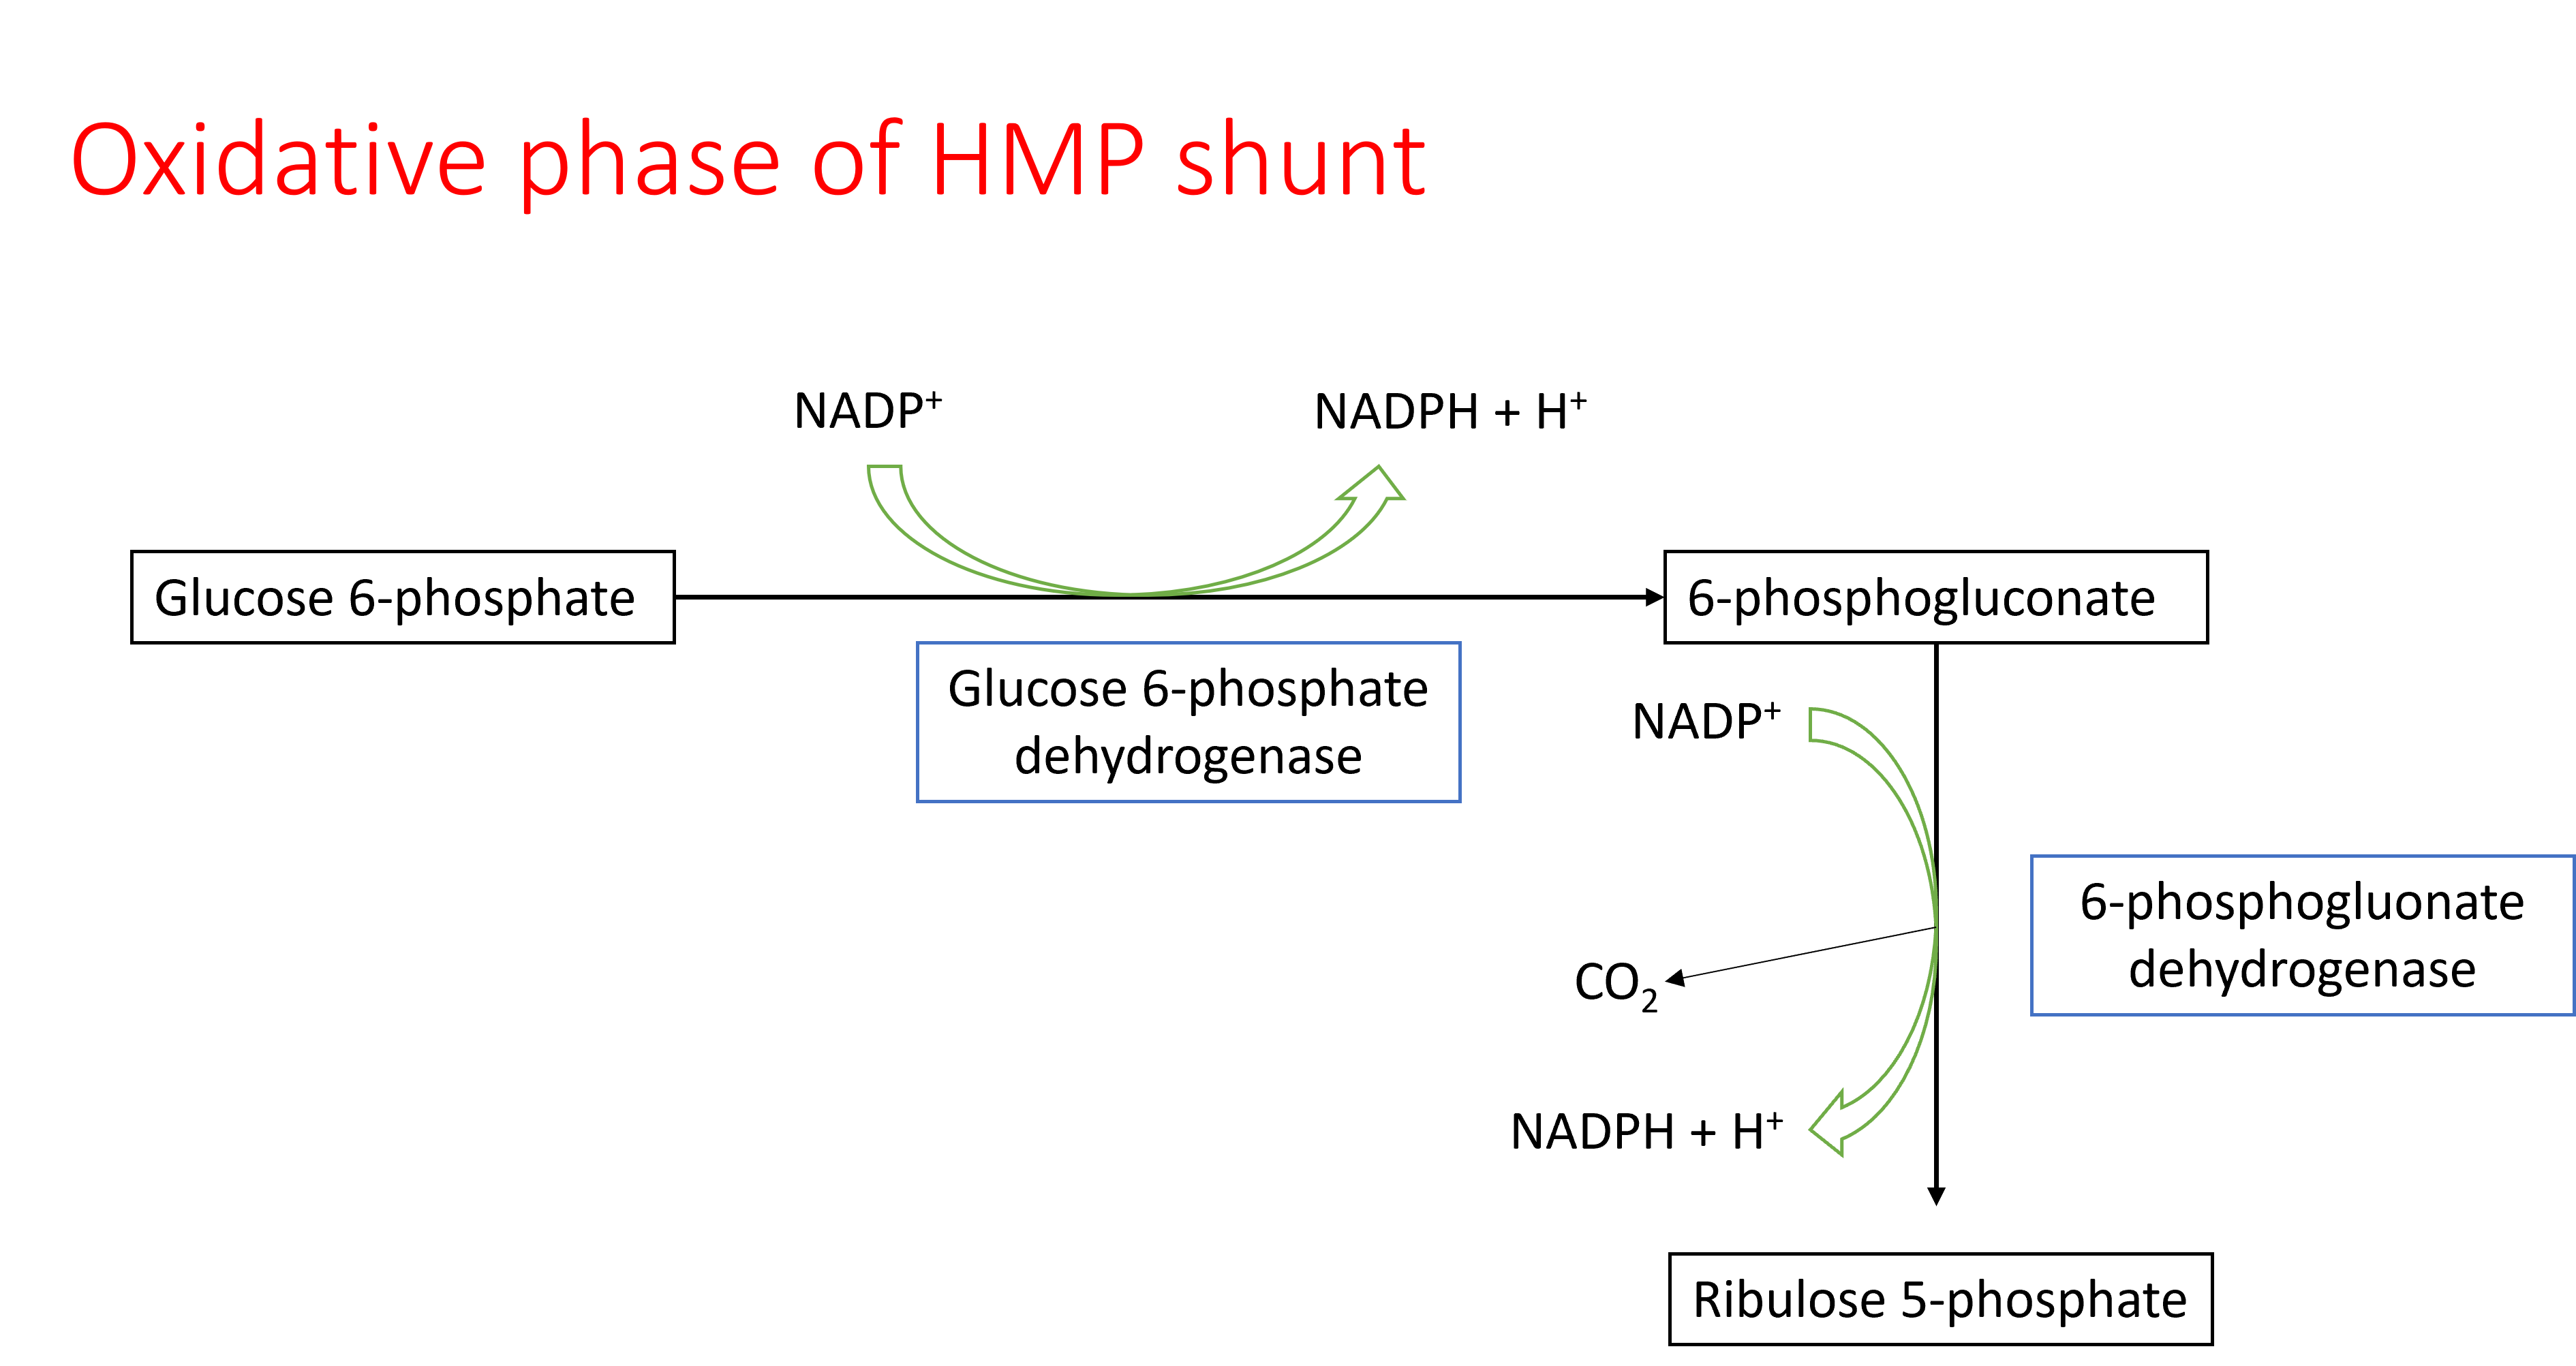
\includegraphics[width=\textwidth,height=3.125in]{Images/hmp1.png}

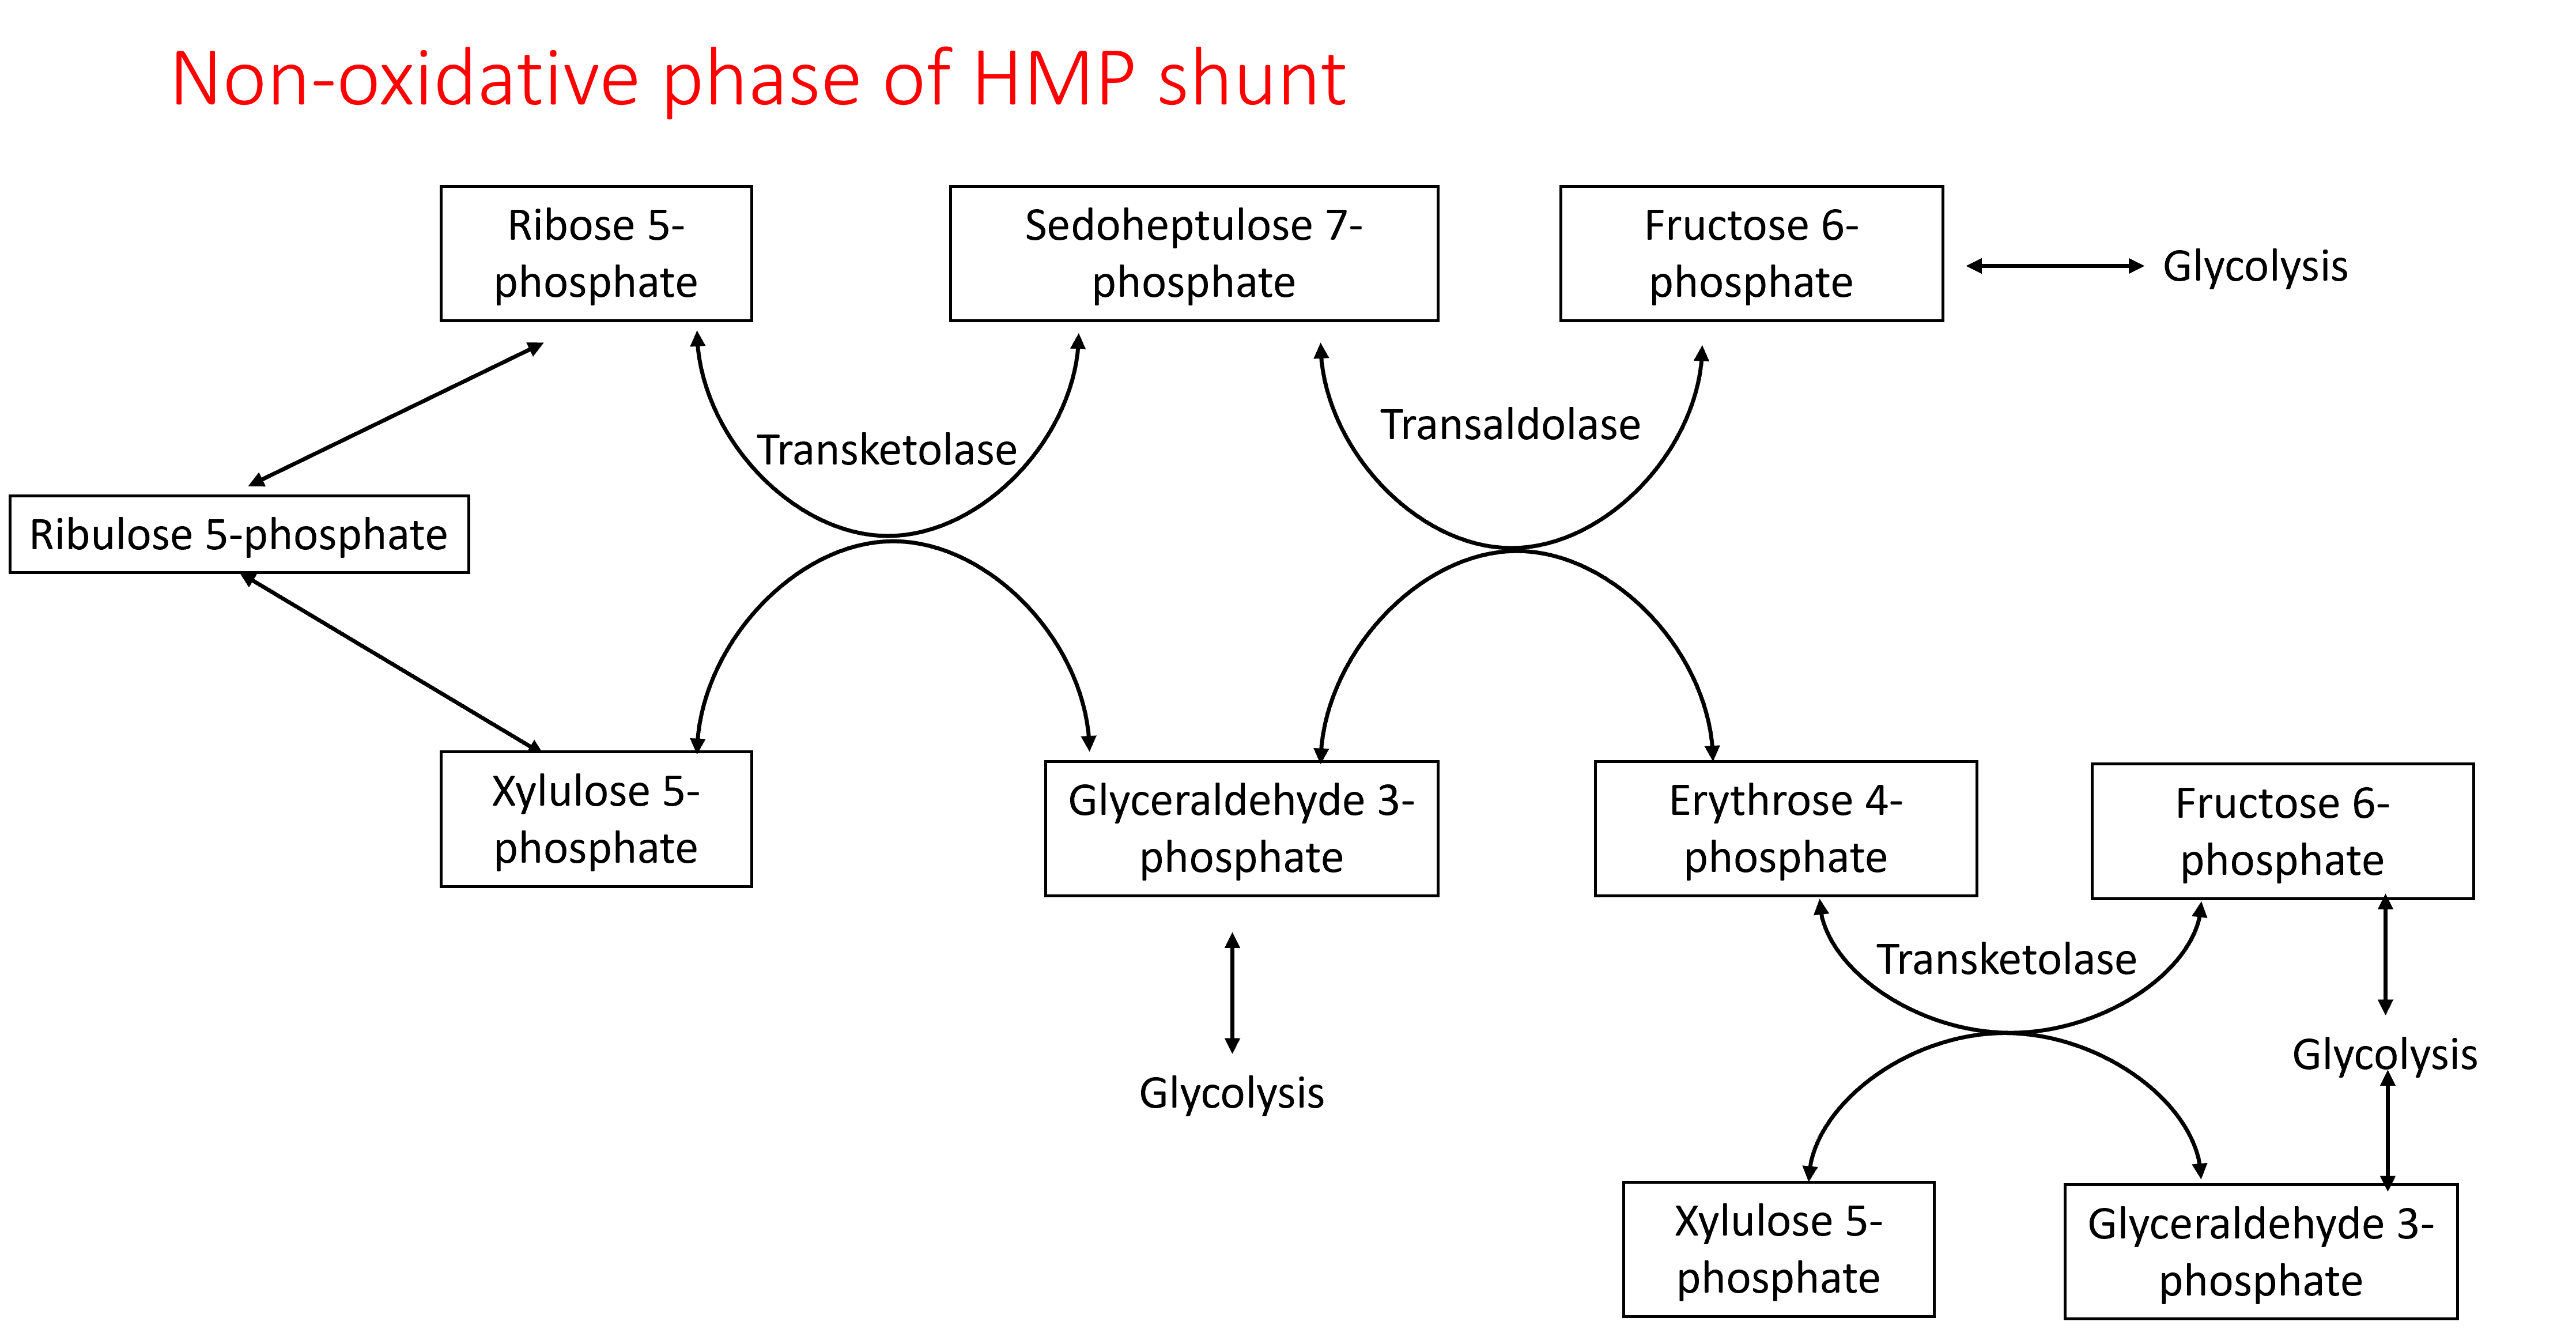
\includegraphics[width=\textwidth,height=3.125in]{Images/hmp2.png}

Ribulose-5 phosphate is converted to ribose-5 phosphate and used by cells if required. If ribose-5 phosphate is not required, the non-oxidative phase of the HMP pathway will convert ribulose-5 phosphate into glycolytic intermediates which could be recycled for either glycolysis or more NADPH production in the oxidative phase.

\section{Importance of the HMP shunt}\label{importance-of-the-hmp-shunt}

\subsection{Ribose}\label{ribose}

Formation of ribose 5-phosphate in all cells for the synthesis of nucleotides

\subsection{Functions of NADPH}\label{functions-of-nadph}

\subsubsection{Reductive biosynthesis}\label{reductive-biosynthesis}

Provides electron (reducing agent) during synthesis of:

\begin{itemize}
\tightlist
\item
  Fatty acids
\item
  Cholesterol
\item
  Steroid hormones
\end{itemize}

\subsubsection{Reducing hydrogen peroxide}\label{reducing-hydrogen-peroxide}

Hydrogen peroxide is a highly reactive oxygen containing molecule that can destroy the contents of the cell by oxidation. Hydrogen peroxide is produced during several physiological processes and due to environmental factors, such as ionizing radiation, pollutants and drugs. Hydrogen peroxide and other such highly reactive oxidants are neutralized by anti-oxidant systems including the Glutathione peroxidase system.

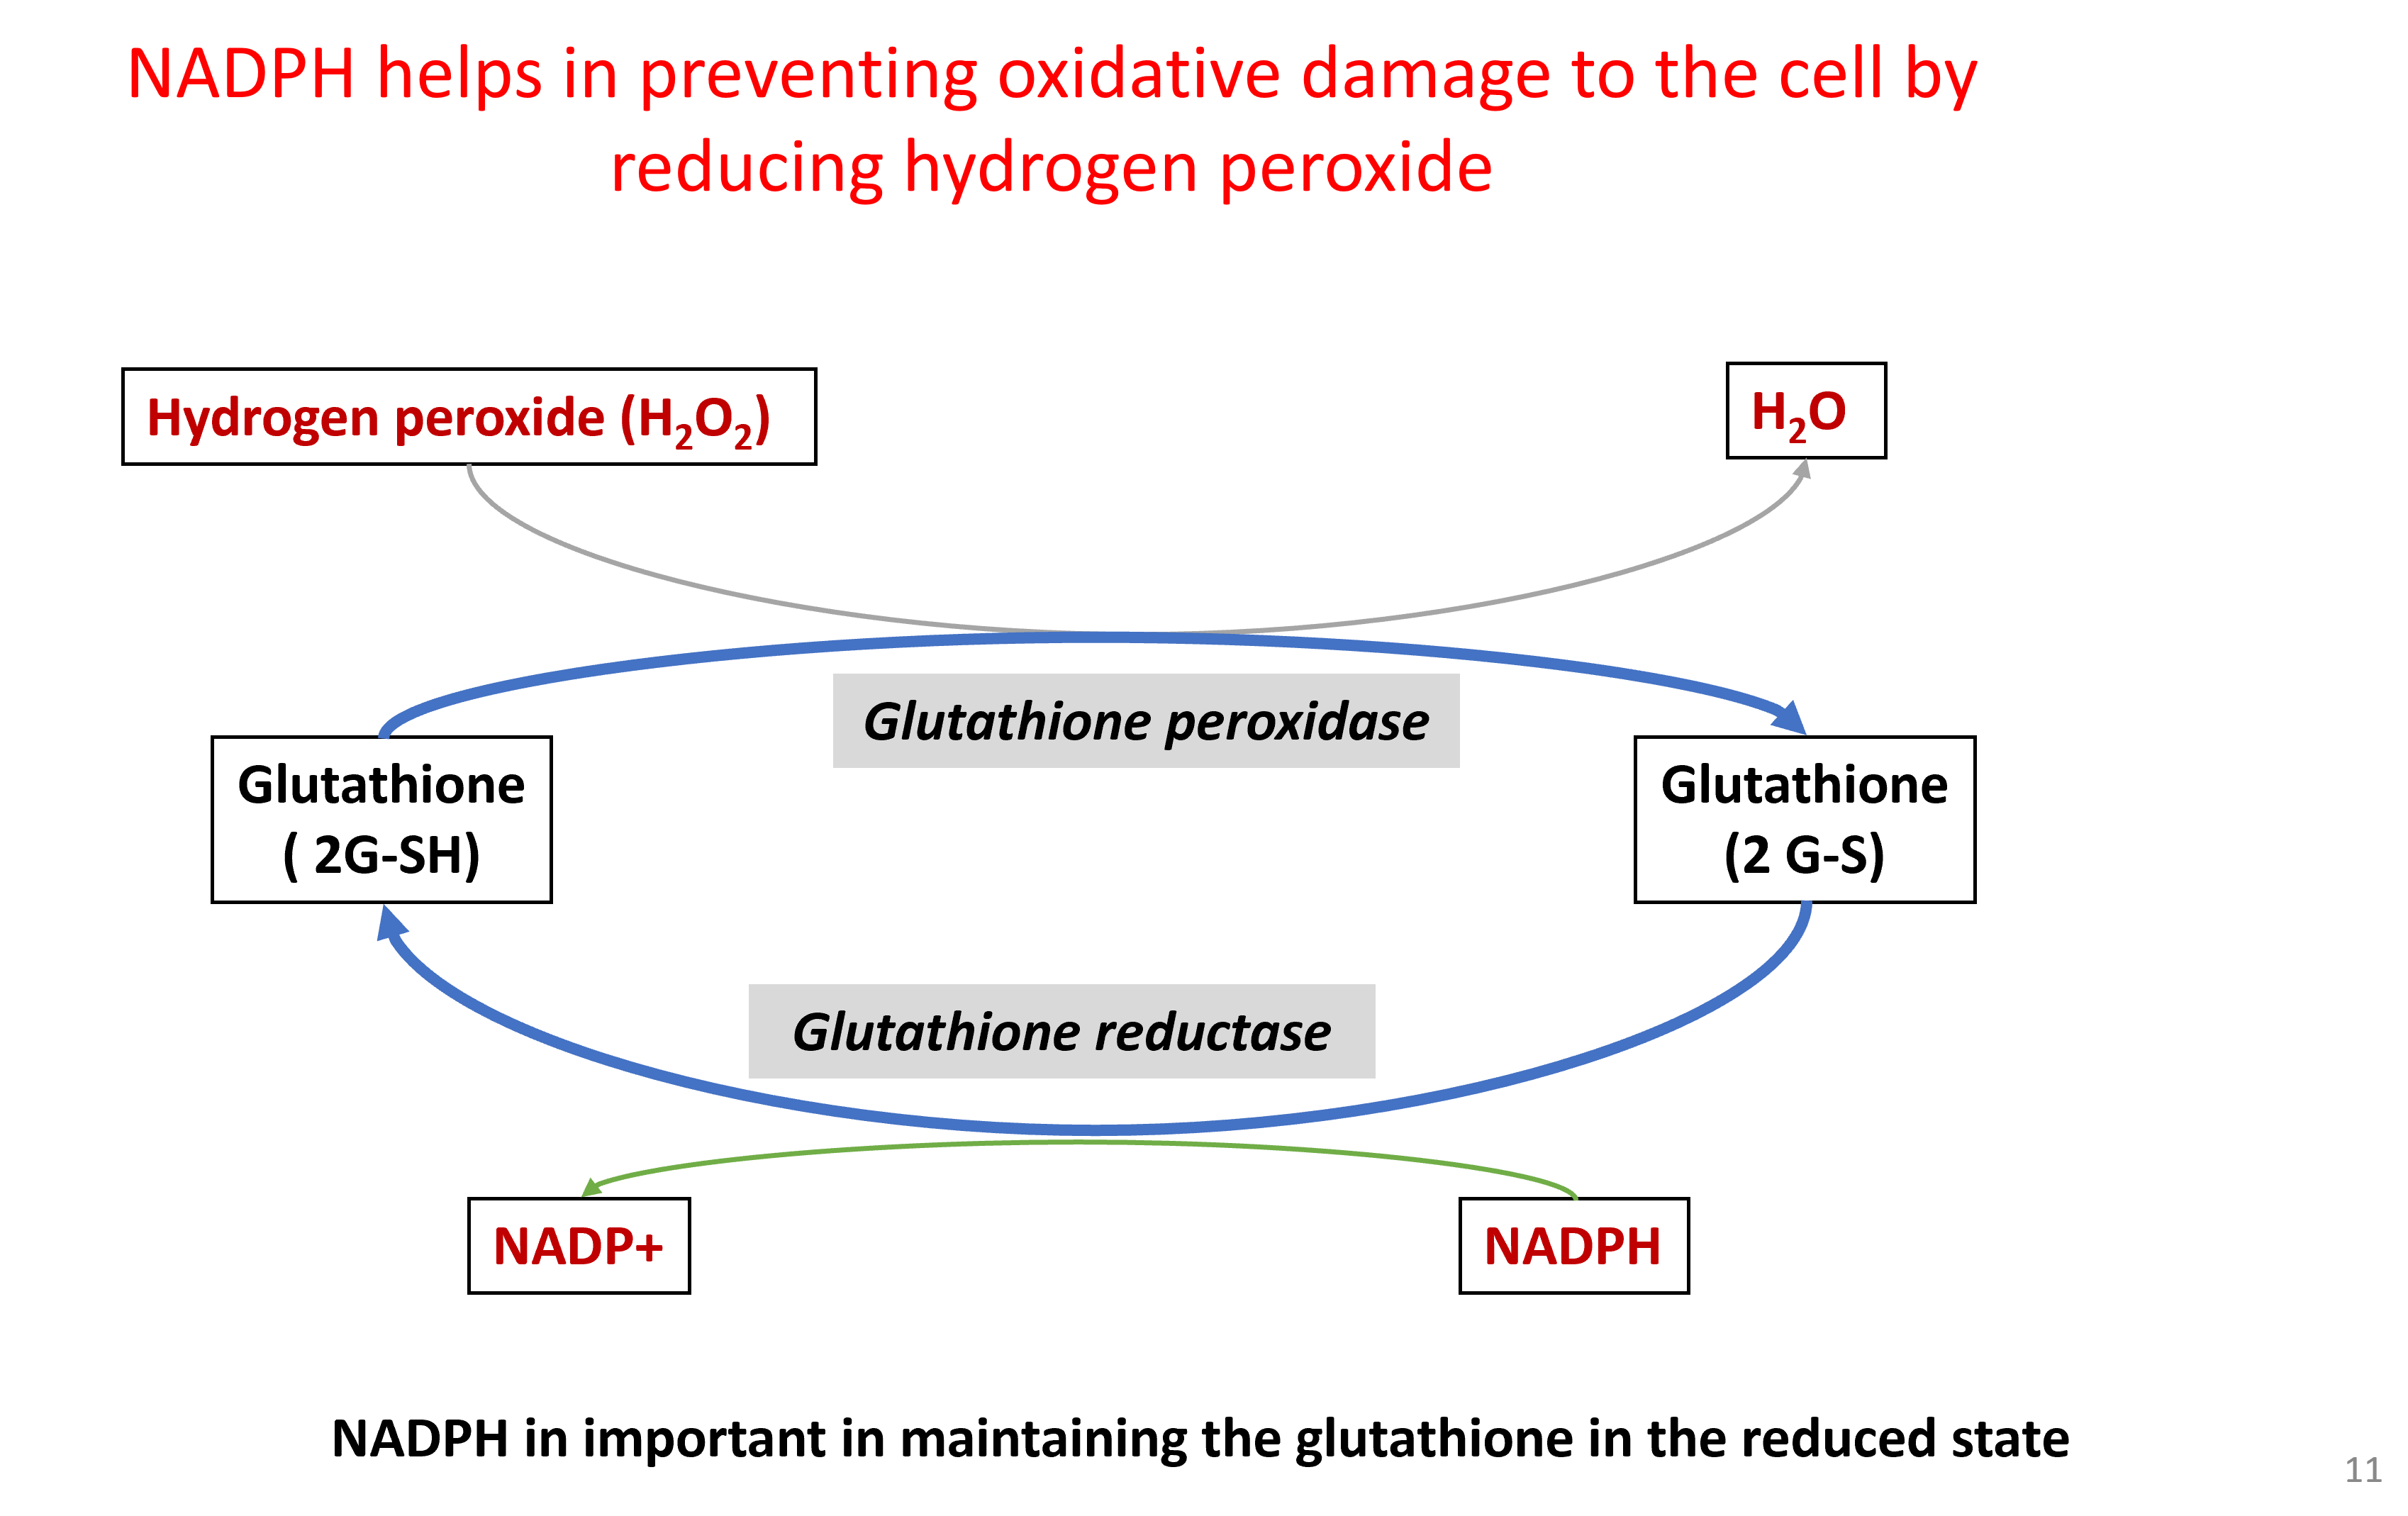
\includegraphics[width=\textwidth,height=4.16667in]{Images/Glutathione.png}

Inability to maintain glutathione in reduced state in RBCs leads to accumulation of peroxides causing damage to the cell membrane. The damage to RBC membrane leads to hemolysis. NADPH prevents this./

\subsubsection{Generation of reactive oxygen species during phagocytosis}\label{generation-of-reactive-oxygen-species-during-phagocytosis}

Macrophages produce reactive oxygen species to destroy bacteria in a process known as respiratory burst. In respiratory burst, NADPH are used as a source of electrons to reduce oxygen to hydrogen peroxide.

\section{G6PD deficiency}\label{g6pd-deficiency}

A common genetic disoder in India and other tropical regions of the world, characterised by defect in the enzyme glucose-6-phosphate dehydrogenase which leads to decreased production of NADPH and increased oxidative stress. In particular, RBCs are more susceptible to oxidative stress and hemolysis.

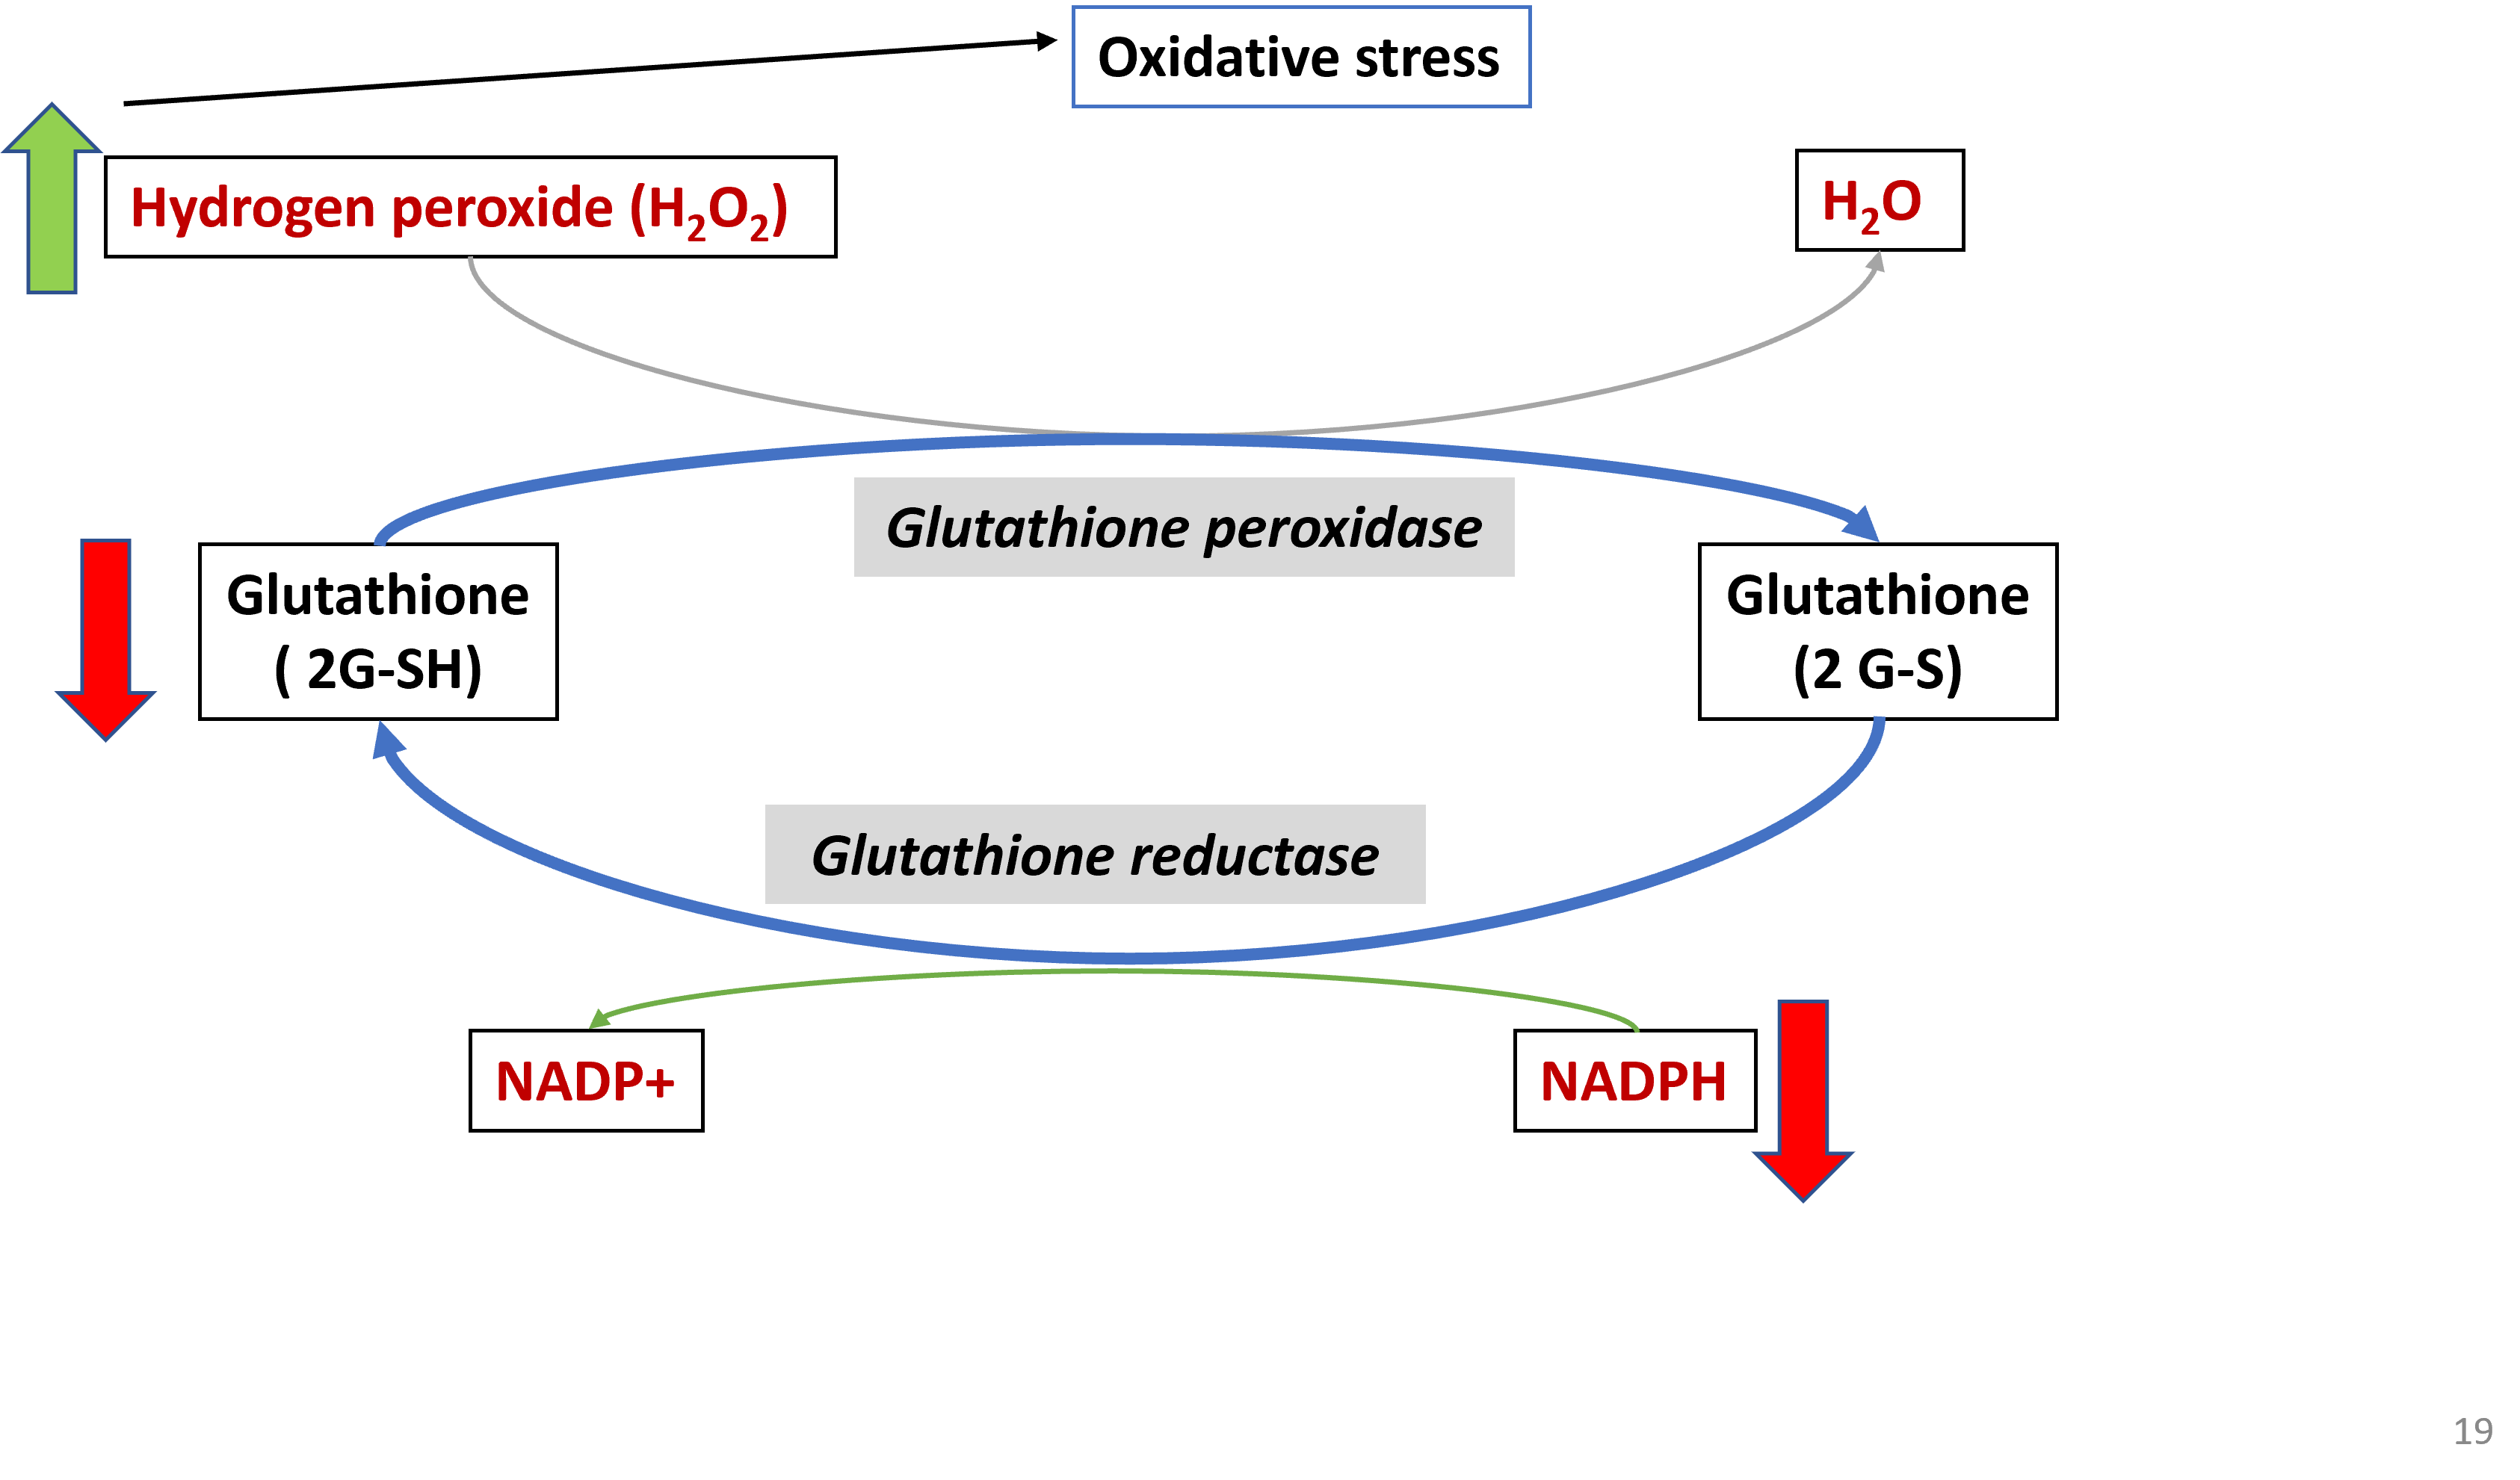
\includegraphics[width=\textwidth,height=4.16667in]{Images/G6PD.png}

\subsection{Clinical manifestations of G6PD deficiency}\label{clinical-manifestations-of-g6pd-deficiency}

\begin{itemize}
\item
  Increased oxidative stress in RBCs destroys the RBC membrane leading to intravascular hemolysis
\item
  Increased oxidative stress can be caused by certain drugs (e.g., primaquine), food items (e.g., fava beans), infections
\item
  Hemolysis leads to anemia
\item
  The end product of heme catabolism is bilirubin and so hemolysis leads to jaundice
\end{itemize}

\chapter{Fructose metabolism}\label{fructose-metabolism}

Fructose is present in fruit juices, honey, cane sugar etc. Cells can use fructose as a fuel directly or after converting it into glucose.

Fructose can enter glycolysis and produce ATP either through hexokinase or through fructokinase and aldolase B.

\section{Fructose metabolism through hexokinase}\label{fructose-metabolism-through-hexokinase}

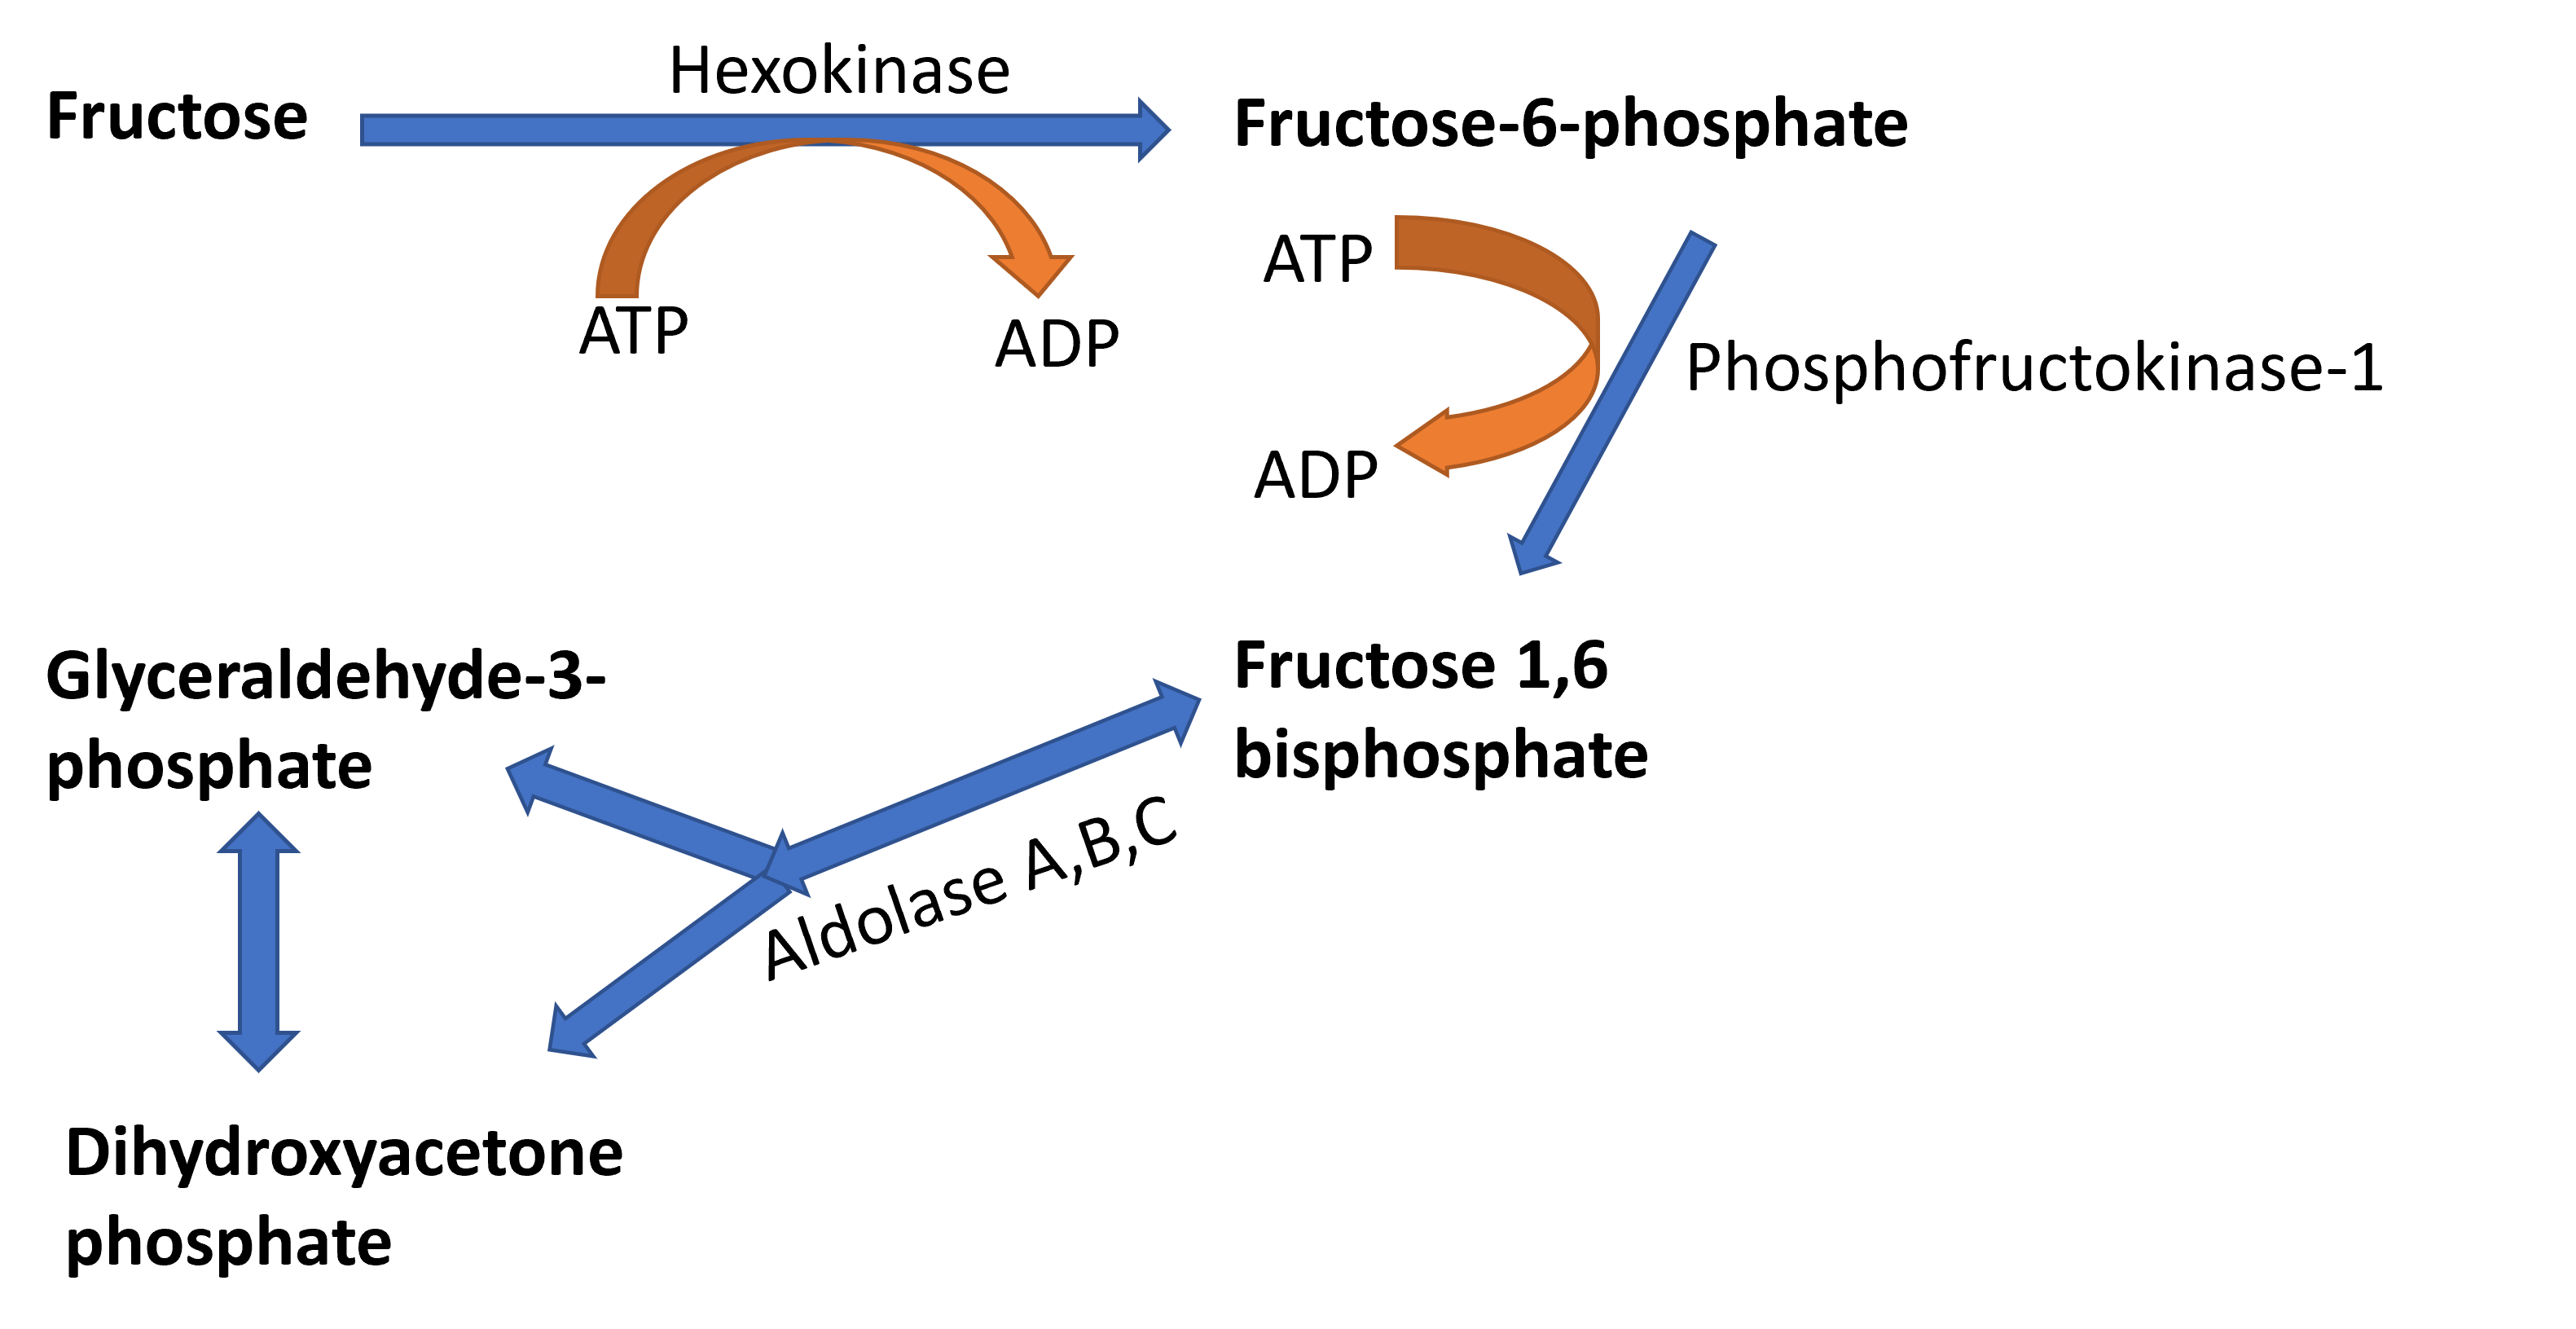
\includegraphics[width=\textwidth,height=4.16667in]{Images/Fructose1.png}

\section{Fructose metabolism through fructokinase and Aldolase B}\label{fructose-metabolism-through-fructokinase-and-aldolase-b}

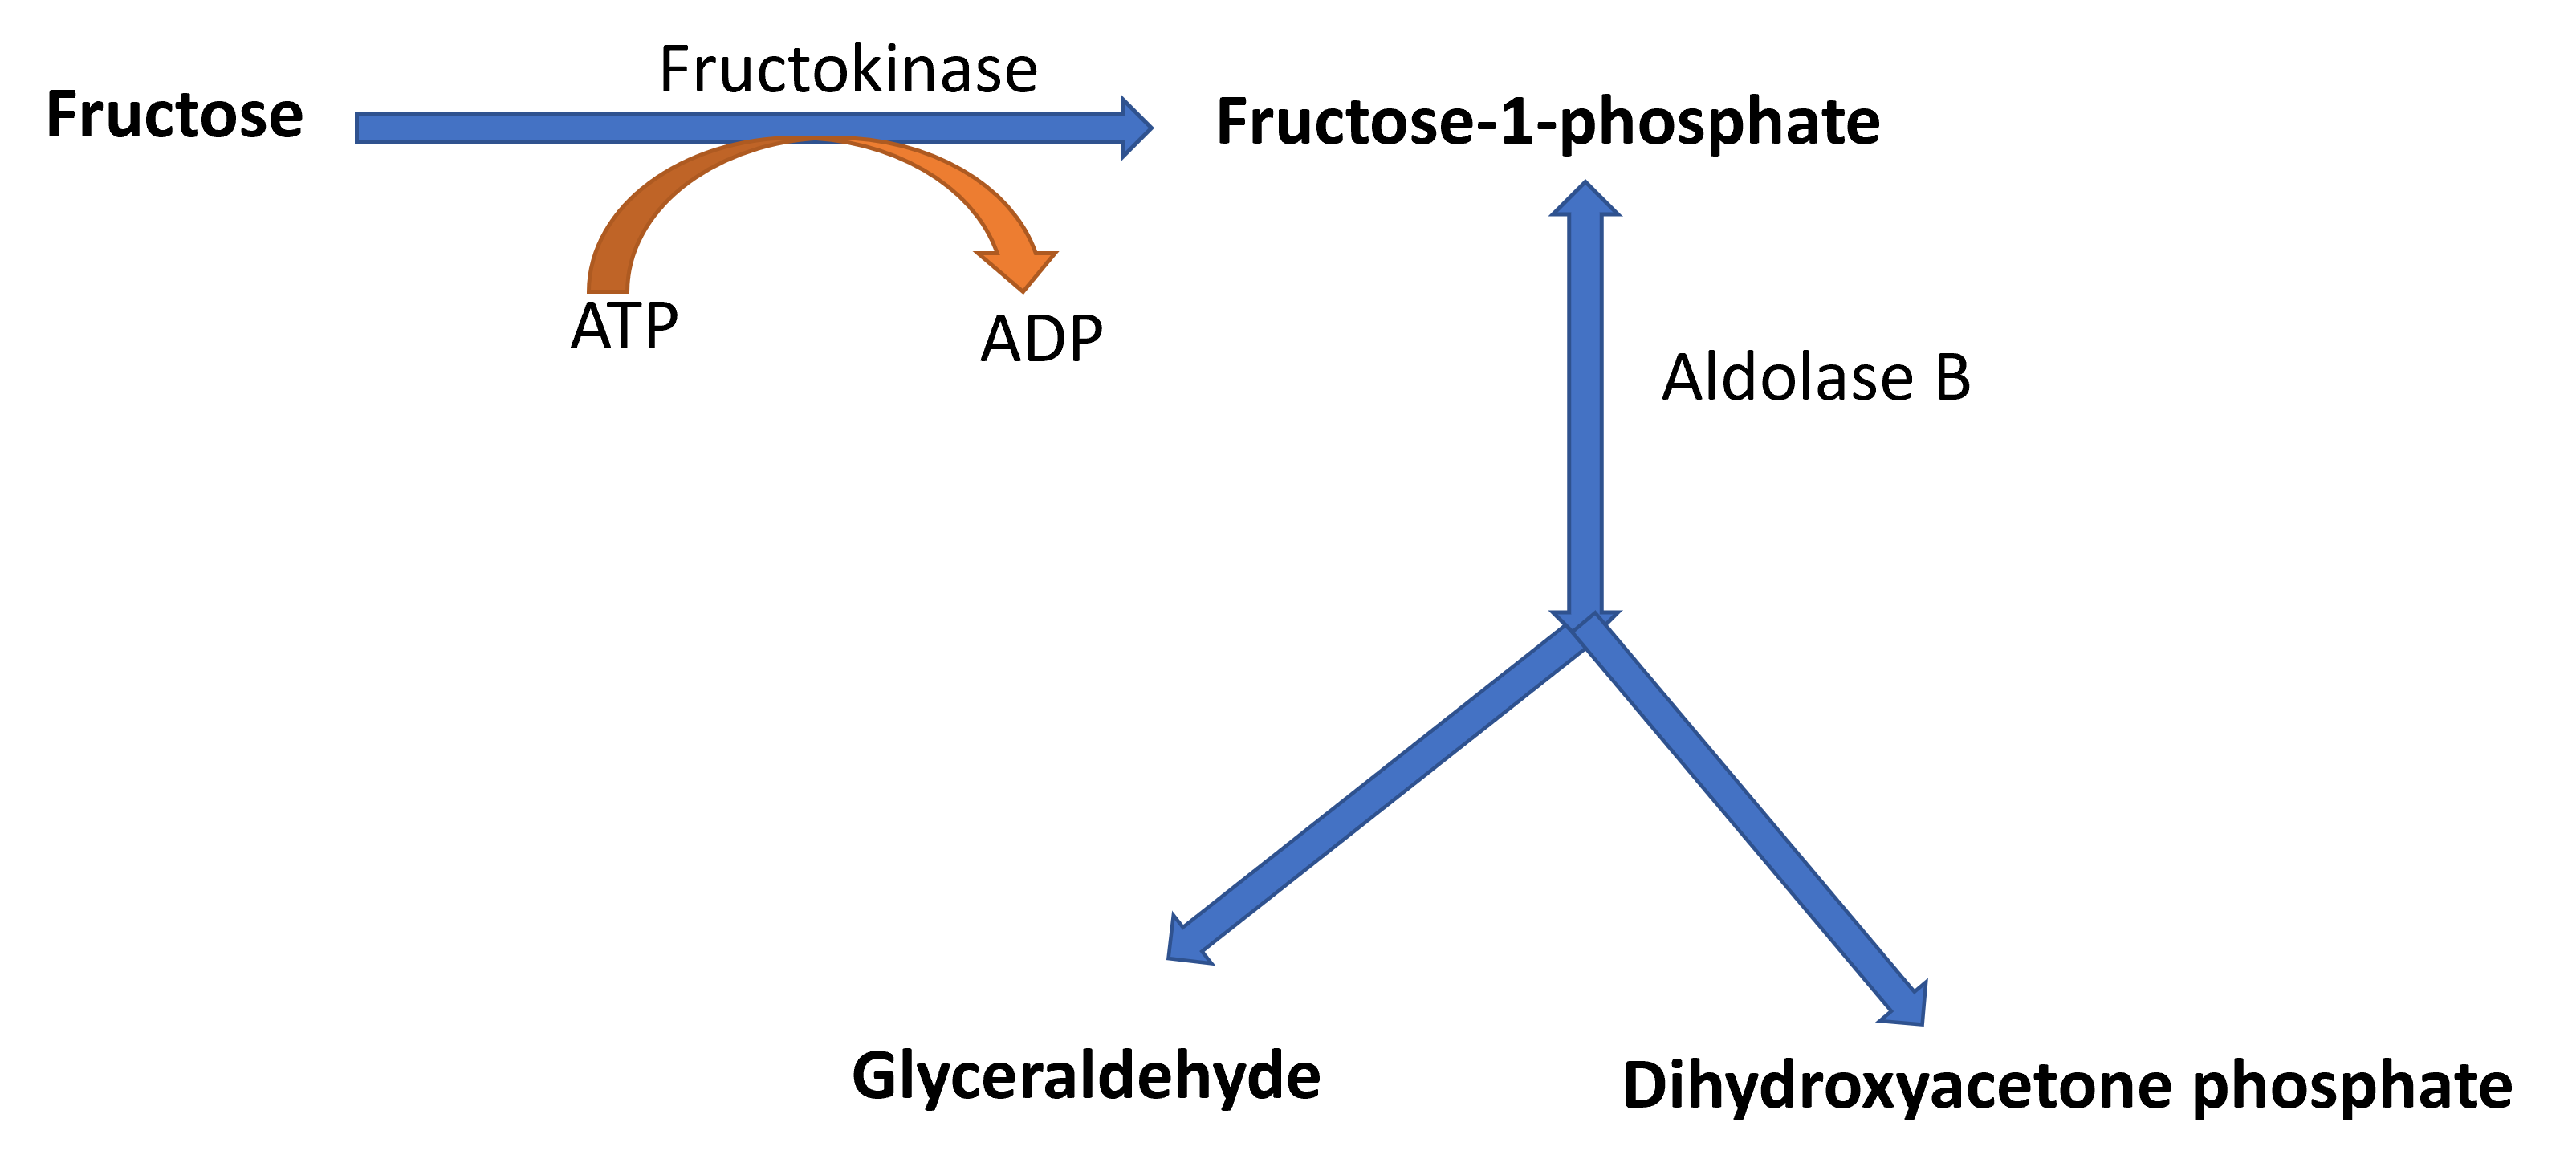
\includegraphics[width=\textwidth,height=4.16667in]{Images/Fructose2.png}

\section{Disorders of fructose metabolism}\label{disorders-of-fructose-metabolism}

\subsection{Essential fructosuria}\label{essential-fructosuria}

Occurs due to genetic defect in the enzyme fructokinase. It is characterized by increased excretion of fructose in urine but it is a benign condition.

\subsection{Hereditary fructose intolerance}\label{hereditary-fructose-intolerance}

Occurs due to genetic defect in the enzyme aldolase B. It is characterized by hypoglycemia, hepatomegaly, jaundice and kidney disease. Symptoms occur due to consumption of inorganic phosphate during the conversion of fructose to fructose-1-phosphate.

\section{Sorbitol pathway}\label{sorbitol-pathway-1}

Glucose can be converted to fructose in liver, testis and seminal vesicles. Fructose produced by the seminal vesicles act as a source of energy for sperm cells. Glucose is first reduced to sorbitol by aldose reductase with the help of NADPH and sorbitol is oxidized to fructose by sorbitol dehydrogenase using NAD\textsuperscript{+}.

Tissues such as lens, and capillarie of retina, kidney and nerves convert glucose to sorbitol when glucose is present at high concentration, but they lack sorbitol dehydrogenase resulting in accumulation of sorbitol. In Diabetes Mellitus, accumulation of sorbitol causes osmotic damage to these tissues leading to cataract, retinopathy, nephropathy and neuropathy.

\chapter{Galactose metabolism}\label{galactose-metabolism}

Galactose is utilized as fuel in cells after being converted into glucose. Galactose is synthesized in mammary glands for production of lactose in milk.

\section{Metabolism of galactose}\label{metabolism-of-galactose}

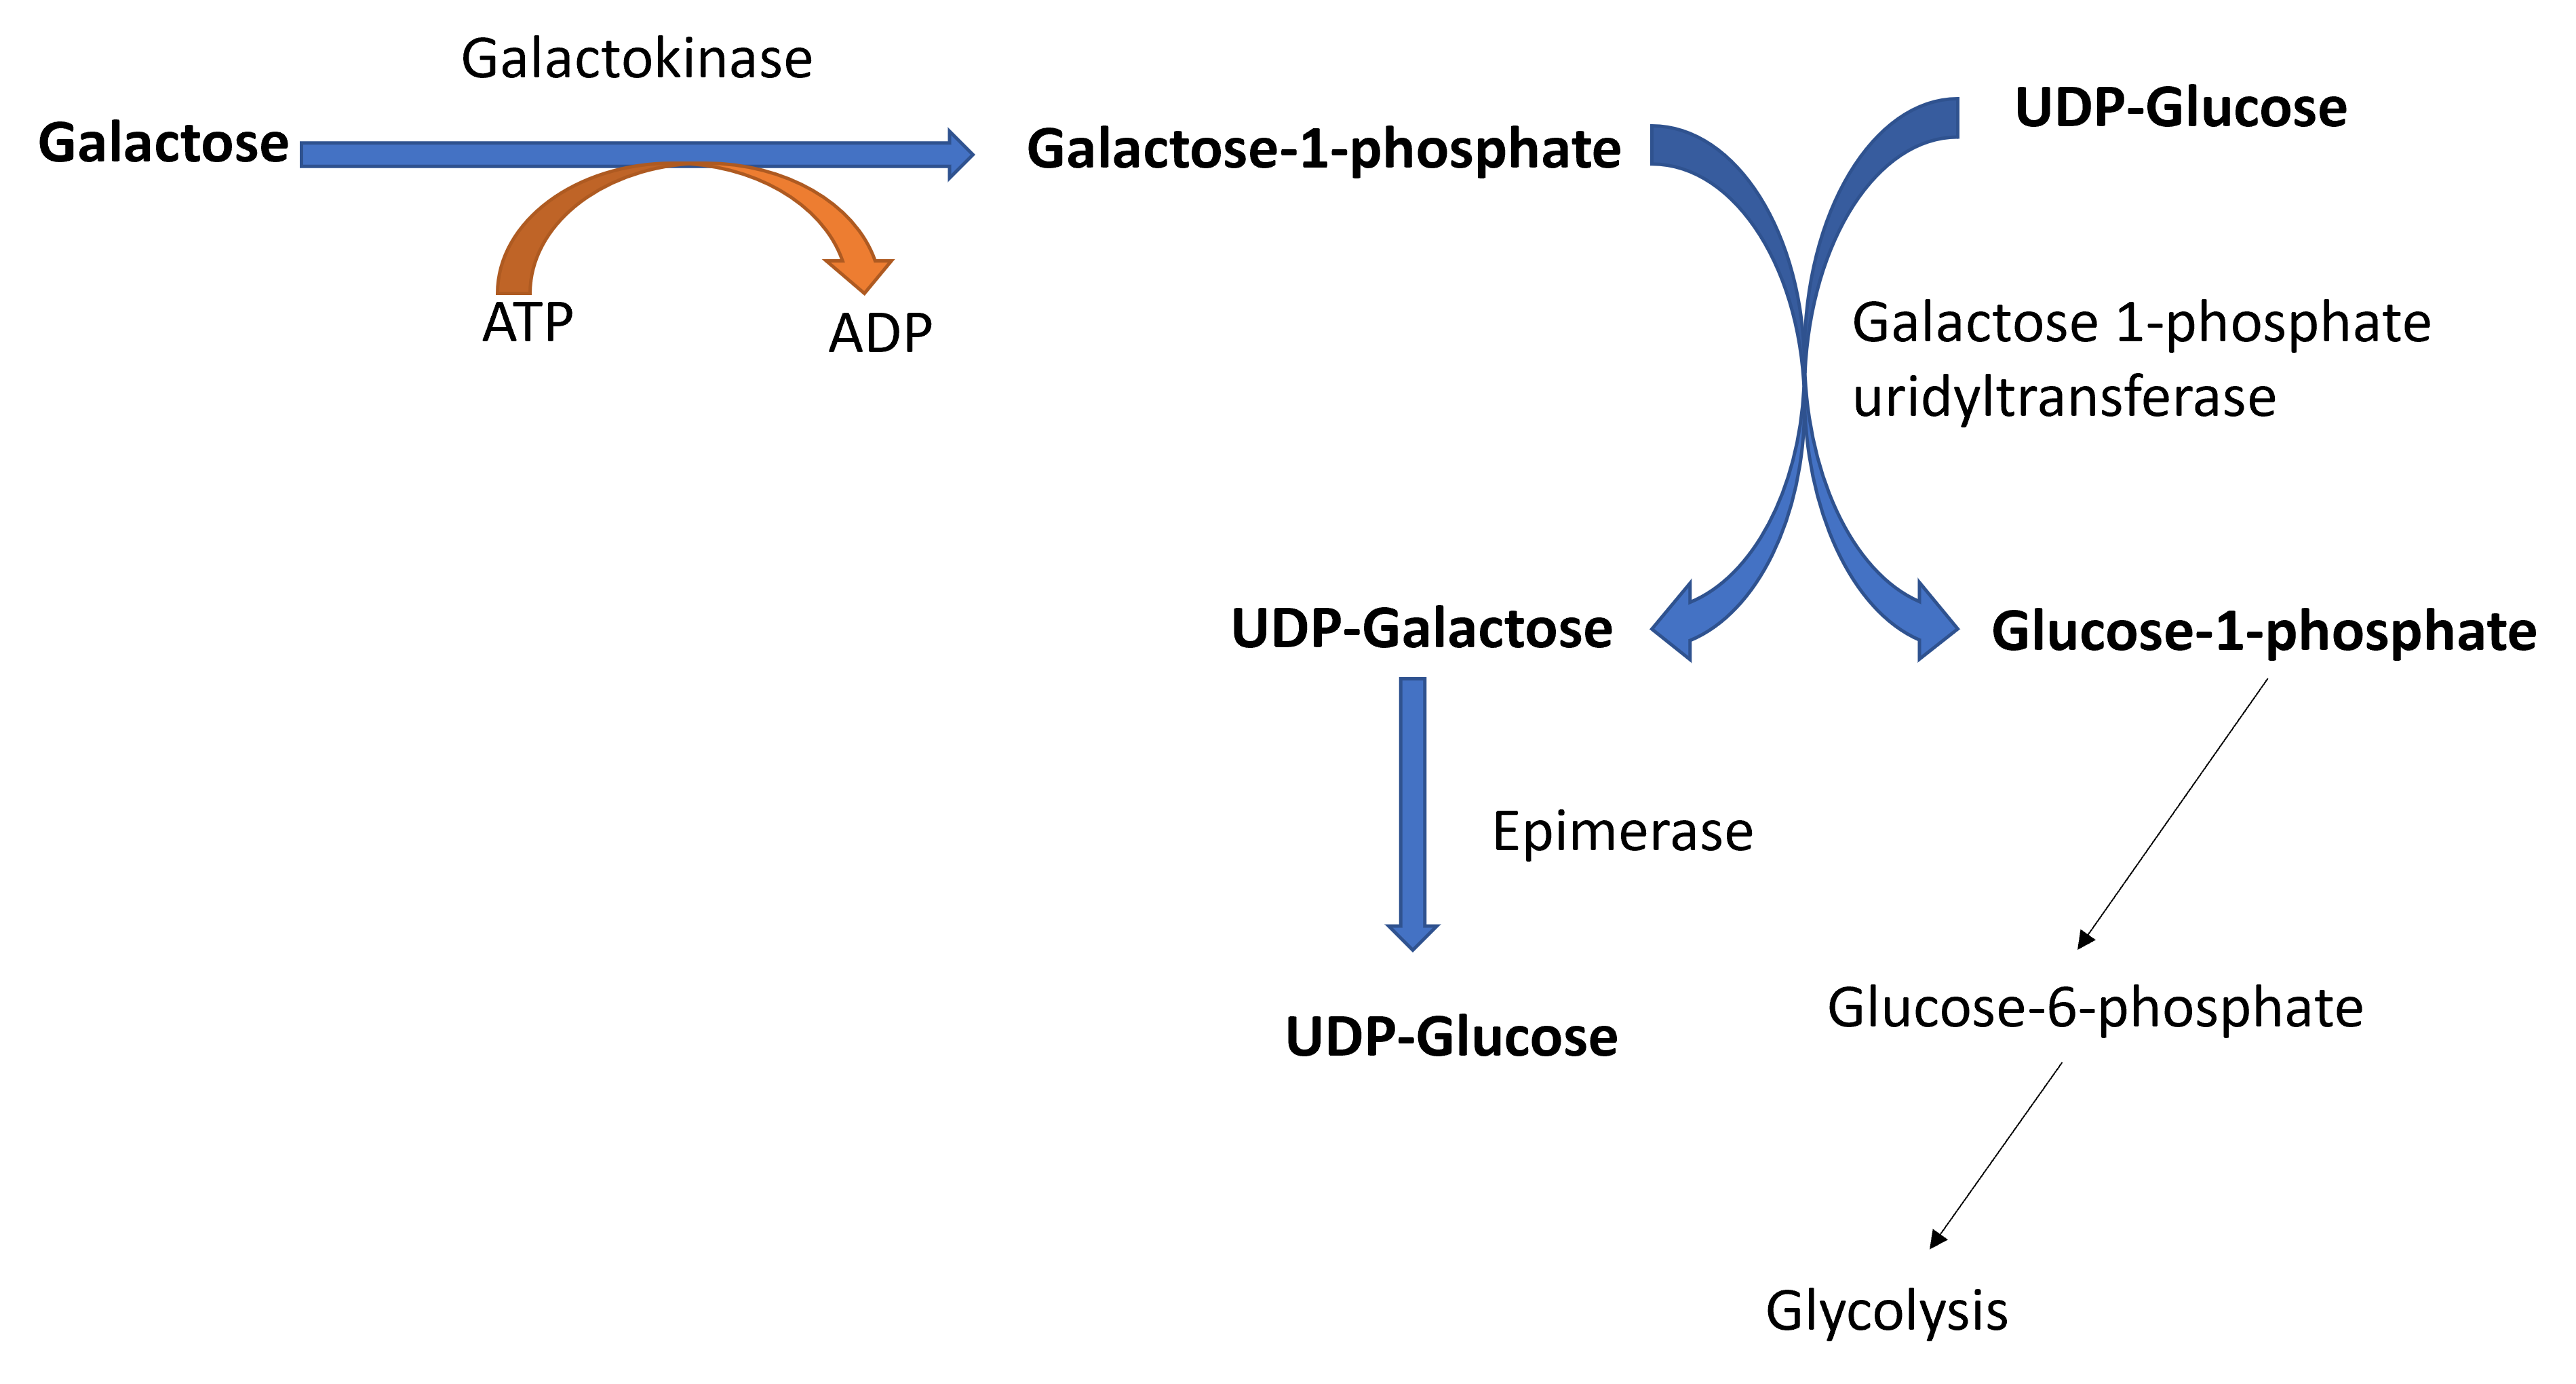
\includegraphics[width=\textwidth,height=3.125in]{Images/Galactose.png}

\section{Disorders of galactose metabolism}\label{disorders-of-galactose-metabolism}

\subsection{Galactokinase deficiency}\label{galactokinase-deficiency}

Leads to increased levels of galactose in blood (galactosemia) and urine (galactosuria).Increased levels of galactose leads to formation of galactitol in lens which causes cataract.

\subsection{Classical galactosemia}\label{classical-galactosemia}

Occurs due to genetic defect in the enzyme Galactose 1-phosphate uridyltransferase. It leads to galactosemia and galactosuria. Increased levels of galactose causes cataract, and accumulation of galactose-1-phosphate damages brain, liver and kidney.

\begin{itemize}
\item
  How do you load the tidyverse package? \_\_\_\_\_\_\_\_\_\_\_\_\_\_\_\_\_\_\_\_
  \#\# Multiple Choice (\texttt{mcq()})
\item
  ``Never gonna give you up, never gonna:
\item
  \begin{enumerate}
  \def\labelenumi{(\Alph{enumi})}
  \tightlist
  \item
    let you go\\
  \end{enumerate}
\item
  \begin{enumerate}
  \def\labelenumi{(\Alph{enumi})}
  \setcounter{enumi}{1}
  \tightlist
  \item
    turn you down\\
  \end{enumerate}
\item
  \begin{enumerate}
  \def\labelenumi{(\Alph{enumi})}
  \setcounter{enumi}{2}
  \tightlist
  \item
    run away\\
  \end{enumerate}
\item
  \begin{enumerate}
  \def\labelenumi{(\Alph{enumi})}
  \setcounter{enumi}{3}
  \tightlist
  \item
    let you down
  \end{enumerate}
\end{itemize}

''
- ``I

\begin{itemize}
\tightlist
\item
  \begin{enumerate}
  \def\labelenumi{(\Alph{enumi})}
  \tightlist
  \item
    bless the rains\\
  \end{enumerate}
\item
  \begin{enumerate}
  \def\labelenumi{(\Alph{enumi})}
  \setcounter{enumi}{1}
  \tightlist
  \item
    guess it rains\\
  \end{enumerate}
\item
  \begin{enumerate}
  \def\labelenumi{(\Alph{enumi})}
  \setcounter{enumi}{2}
  \tightlist
  \item
    sense the rain
  \end{enumerate}
\end{itemize}

down in Africa'' -Toto
\#\# True or False (\texttt{torf()})
- True or False? You can permute values in a vector using \texttt{sample()}. TRUE / FALSE
\#\# Longer MCQs (\texttt{longmcq()})
When your answers are very long, sometimes a drop-down select box gets formatted oddly. You can use \texttt{longmcq()} to deal with this. Since the answers are long, It's probably best to set up the options inside an R chunk with \texttt{echo=FALSE}.
\textbf{What is a p-value?}

\begin{itemize}
\tightlist
\item
  \begin{enumerate}
  \def\labelenumi{(\Alph{enumi})}
  \tightlist
  \item
    the probability that the null hypothesis is true\\
  \end{enumerate}
\item
  \begin{enumerate}
  \def\labelenumi{(\Alph{enumi})}
  \setcounter{enumi}{1}
  \tightlist
  \item
    the probability of the observed, or more extreme, data, under the assumption that the null-hypothesis is true\\
  \end{enumerate}
\item
  \begin{enumerate}
  \def\labelenumi{(\Alph{enumi})}
  \setcounter{enumi}{2}
  \tightlist
  \item
    the probability of making an error in your conclusion
  \end{enumerate}
\end{itemize}

  \bibliography{book.bib,packages.bib}

\end{document}
